% defer/defer.tex

\QuickQuizChapter{chp:Deferred Processing}{Deferred Processing}

The strategy of deferring work goes back before the dawn of recorded
history. It has occasionally been derided as procrastination or
even as sheer laziness.
However, in the last few decades workers have recognized this strategy's value
in simplifying and streamlining parallel algorithms~\cite{Kung80,HMassalinPhD}.
Believe it or not, ``laziness'' in parallel programming often outperforms and
scales better than does industriousness!
General approaches to such work deferral tactics include
reference counting, sequence locking, and RCU.

% defer/refcnt.tex
% mainfile: ../perfbook.tex
% SPDX-License-Identifier: CC-BY-SA-3.0

\section{Reference Counting}
\label{sec:defer:Reference Counting}
%
\epigraph{I am never letting you go!}{Unknown}

\begin{listing}[tbp]
\input{CodeSamples/defer/route_refcnt@lookup.fcv}
\caption{Reference-Counted Pre-BSD Routing Table Lookup (BUGGY!!!)}
\label{lst:defer:Reference-Counted Pre-BSD Routing Table Lookup}
\end{listing}

\begin{listing}[tbp]
\input{CodeSamples/defer/route_refcnt@add_del.fcv}
\caption{Reference-Counted Pre-BSD Routing Table Add\slash Delete (BUGGY!!!)}
\label{lst:defer:Reference-Counted Pre-BSD Routing Table Add/Delete}
\end{listing}

Reference counting tracks the number of references to a given object in
order to prevent that object from being prematurely freed.
As such, it has a long and honorable history of use dating back to
at least the early
1960s~\cite{Weizenbaum:1963:SLP:367593.367617}.\footnote{
	Weizenbaum discusses reference counting as if it was already
	well-known, so it likely dates back to the 1950s and perhaps
	even to the 1940s.
	And perhaps even further.
	People repairing and maintaining large dangerous machines have long
	used a mechanical reference-counting technique implemented via
	padlocks.
	Before entering the machine, each worker locks a padlock onto
	the machine's on/off switch, thus preventing the machine from
	being powered on while that worker is inside.}
Reference counting is thus an excellent candidate for a concurrent
implementation of Pre-BSD routing.

To that end,
Listing~\ref{lst:defer:Reference-Counted Pre-BSD Routing Table Lookup}
shows data structures and the \co{route_lookup()} function and
Listing~\ref{lst:defer:Reference-Counted Pre-BSD Routing Table Add/Delete}
shows the \co{route_add()} and \co{route_del()} functions
(all at \path{route_refcnt.c}).
Since these algorithms are quite similar to the sequential algorithm
shown in
Listing~\ref{lst:defer:Sequential Pre-BSD Routing Table},
only the differences will be discussed.

\begin{lineref}[ln:defer:route_refcnt:lookup:entry]
Starting with
Listing~\ref{lst:defer:Reference-Counted Pre-BSD Routing Table Lookup},
line~\lnref{refcnt} adds the actual reference counter,
line~\lnref{freed} adds a \co{->re_freed}
use-after-free check field,
line~\lnref{routelock} adds the \co{routelock} that will
be used to synchronize concurrent updates,
\end{lineref}
\begin{lineref}[ln:defer:route_refcnt:lookup:re_free]
and lines~\lnref{b}-\lnref{e} add \co{re_free()}, which sets
\co{->re_freed}, enabling \co{route_lookup()} to check for
use-after-free bugs.
\end{lineref}
\begin{lineref}[ln:defer:route_refcnt:lookup:lookup]
In \co{route_lookup()} itself,
lines~\lnref{relprev:b}-\lnref{relprev:e} release the reference
count of the prior element and free it if the count becomes zero,
and lines~\lnref{acq:b}-\lnref{acq:e} acquire a reference on the new element,
with lines~\lnref{check_uaf}
and~\lnref{abort} performing the use-after-free check.
\end{lineref}

\QuickQuiz{}
	Why bother with a use-after-free check?
\QuickQuizAnswer{
	To greatly increase the probability of finding bugs.
	A small torture-test program
	(\path{routetorture.h}) that allocates and frees only
	one type of structure can tolerate a surprisingly
	large amount of use-after-free misbehavior.
	See Figure~\ref{fig:debugging:Number of Tests Required for 99 Percent Confidence Given Failure Rate}
	on page~\pageref{fig:debugging:Number of Tests Required for 99 Percent Confidence Given Failure Rate}
	and the related discussion in
	Section~\ref{sec:debugging:Hunting Heisenbugs}
	starting on
	page~\pageref{sec:debugging:Hunting Heisenbugs}
	for more on the importance
	of increasing the probability of finding bugs.
} \QuickQuizEnd

\begin{lineref}[ln:defer:route_refcnt:add_del]
In Listing~\ref{lst:defer:Reference-Counted Pre-BSD Routing Table Add/Delete},
lines~\lnref{acq1}, \lnref{rel1}, \lnref{acq2}, \lnref{rel2},
and~\lnref{rel3} introduce locking to synchronize
concurrent updates.
Line~\lnref{init:freed} initializes the \co{->re_freed} use-after-free-check field,
and finally lines~\lnref{re_free:b}-\lnref{re_free:e} invoke
\co{re_free()} if the new value of
the reference count is zero.
\end{lineref}

\QuickQuiz{}
	Why doesn't \co{route_del()} in
	Listing~\ref{lst:defer:Reference-Counted Pre-BSD Routing Table Add/Delete}
	use reference counts to
	protect the traversal to the element to be freed?
\QuickQuizAnswer{
	Because the traversal is already protected by the lock, so
	no additional protection is required.
} \QuickQuizEnd

\begin{figure}[tb]
\centering
\resizebox{2.5in}{!}{\includegraphics{CodeSamples/defer/perf-refcnt}}
\caption{Pre-BSD Routing Table Protected by Reference Counting}
\label{fig:defer:Pre-BSD Routing Table Protected by Reference Counting}
\end{figure}

Figure~\ref{fig:defer:Pre-BSD Routing Table Protected by Reference Counting}
shows the performance and scalability of reference counting on a
read-only workload with a ten-element list running on a
single-socket four-core hyperthreaded 2.5\,GHz x86 system.
The ``ideal'' trace was generated by running the sequential code shown in
Listing~\ref{lst:defer:Sequential Pre-BSD Routing Table},
which works only because this is a read-only workload.
The reference-counting performance is abysmal and its scalability even
more so, with the ``refcnt'' trace dropping down onto the x-axis.
This should be no surprise in view of
Chapter~\ref{chp:Hardware and its Habits}:
The reference-count acquisitions and releases have added frequent
shared-memory writes to an otherwise read-only workload, thus
incurring severe retribution from the laws of physics.
As well it should, given that all the wishful thinking in the world
is not going to increase the speed of light or decrease the size of
the atoms used in modern digital electronics.

\QuickQuiz{}
	Why the stairsteps in the ``ideal'' line in
	Figure~\ref{fig:defer:Pre-BSD Routing Table Protected by Reference Counting}?
	Shouldn't it be a straight line?
\QuickQuizAnswer{
	The stair-steps are due to hyperthreading.
	On this particular system, the hardware threads in a given
	core have consecutive CPU numbers.
	In addition, this particular pointer-following
	low-cache-miss-rate workload seems
	to allow a single hardware thread to consume most of the
	relevant resources within its core.
	Workloads featuring heavier computational loads should be
	expected to gain greater benefit from each core's second
	hardware thread.
} \QuickQuizEnd

\QuickQuiz{}
	Why, in these modern times, does
	Figure~\ref{fig:defer:Pre-BSD Routing Table Protected by Reference Counting}
	only go up to 8 CPUs???
\QuickQuizAnswer{
	Given the horrible scalability of reference counting, who needs
	more than eight CPUs?
	Four CPUs would have sufficed to make the point!
	However, people wanting more CPUs are urged to refer to
	Chapter~\ref{chp:Data Structures}.
} \QuickQuizEnd

But it gets worse.

Running multiple updater threads repeatedly invoking
\co{route_add()} and \co{route_del()} will quickly encounter the
\co{abort()} statement on
line~\ref{ln:defer:route_refcnt:lookup:lookup:abort} of
Listing~\ref{lst:defer:Reference-Counted Pre-BSD Routing Table Lookup},
which indicates a use-after-free bug.
This in turn means that the reference counts are not only profoundly
degrading scalability and performance, but also failing to provide
the needed protection.

One sequence of events leading to the use-after-free bug is as follows,
given the list shown in
Figure~\ref{fig:defer:Pre-BSD Packet Routing List}:

\begin{lineref}[ln:defer:route_refcnt:lookup]
\begin{enumerate}
\item	Thread~A looks up address~42, reaching
	line~\lnref{lookup:check_NULL} of
	\co{route_lookup()} in
	Listing~\ref{lst:defer:Reference-Counted Pre-BSD Routing Table Lookup}.
	In other words, Thread~A has a pointer to the first element,
	but has not yet acquired a reference to it.
\item	Thread~B invokes \co{route_del()} in
	Listing~\ref{lst:defer:Reference-Counted Pre-BSD Routing Table Add/Delete}
	to delete the route entry for address~42.
	It completes successfully, and because this entry's \co{->re_refcnt}
	field was equal to the value one, it invokes
	\co{re_free()} to set the \co{->re_freed} field and to free the entry.
\item	Thread~A continues execution of \co{route_lookup()}.
	Its \co{rep} pointer is non-\co{NULL}, but
	line~\lnref{lookup:check_uaf} sees that
	its \co{->re_freed} field is non-zero,
        so line~\lnref{lookup:abort} invokes
	\co{abort()}.
\end{enumerate}
\end{lineref}

The problem is that the reference count is located in the object
to be protected, but that means that there is no protection during
the instant in time when the reference count itself is being acquired!
This is the reference-counting counterpart of a locking issue noted
by Gamsa et al.~\cite{Gamsa99}.
One could imagine using a global lock or reference count to protect
the per-route-entry reference-count acquisition, but this would
result in severe contention issues.
Although algorithms exist that allow safe reference-count acquisition
in a concurrent environment~\cite{Valois95a}, they are not only extremely
complex and error-prone~\cite{MagedMichael95a}, but also provide
terrible performance and scalability~\cite{ThomasEHart2007a}.

In short, concurrency has most definitely reduced the usefulness
of reference counting!

\QuickQuiz{}
	If concurrency has ``most definitely reduced the usefulness
	of reference counting'', why are there so many reference
	counters in the Linux kernel?
\QuickQuizAnswer{
	That sentence did say ``reduced the usefulness'', not
	``eliminated the usefulness'', now didn't it?

	Please see
	Section~\ref{sec:together:Refurbish Reference Counting},
	which discusses some of the techniques that the Linux kernel
	uses to take advantage of reference counting in a highly
	concurrent environment.
} \QuickQuizEnd

That said, sometimes it is necessary to look at a problem in an
entirely different way in order to successfully solve it.
The next section describes what could be thought of as an
inside-out reference count that provides decent performance
and scalability.

% defer/seqlock.tex

\section{Sequence Locks}
\label{sec:defer:Sequence Locks}

\begin{figure}[tb]
\centering
\resizebox{3in}{!}{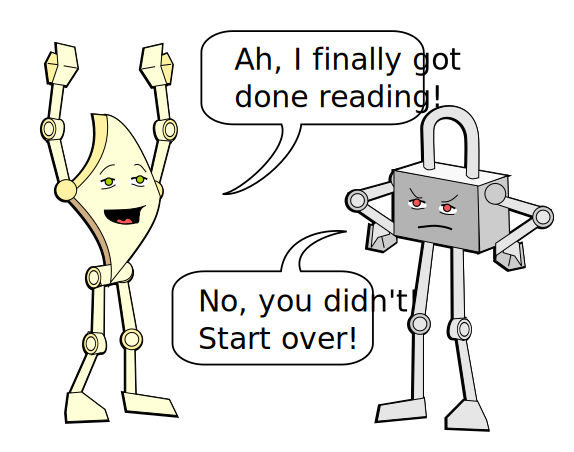
\includegraphics{cartoons/r-2014-Start-over}}
\caption{Reader And Uncooperative Sequence Lock}
\label{fig:defer:Reader And Uncooperative Sequence Lock}
\end{figure}

Sequence locks are used in the Linux kernel for read-mostly data that
must be seen in a consistent state by readers.
However, unlike reader-writer locking, readers do not exclude writers.
Instead, like hazard pointers, sequence locks force readers to
\emph{retry} an operation if they detect activity from a concurrent writer.
As can be seen from
Figure~\ref{fig:defer:Reader And Uncooperative Sequence Lock},
it is important to design code using sequence locks so that readers
very rarely need to retry.

\QuickQuiz{}
	Why isn't this sequence-lock discussion in Chapter~\ref{chp:Locking},
	you know, the one on \emph{locking}?
\QuickQuizAnswer{
	The sequence-lock mechanism is really a combination of two
	separate synchronization mechanisms, sequence counts and
	locking.
	In fact, the sequence-count mechanism is available separately
	in the Linux kernel via the
	\co{write_seqcount_begin()} and \co{write_seqcount_end()}
	primitives.

	However, the combined \co{write_seqlock()} and
	\co{write_sequnlock()} primitives are used much more heavily
	in the Linux kernel.
	More importantly, many more people will understand what you
	mean if you say ``sequence lock'' than if you say
	``sequence count''.

	So this section is entitled ``Sequence Locks'' so that people
	will understand what it is about just from the title, and
	it appears in the ``Deferred Processing'' because (1) of the
	emphasis on the ``sequence count'' aspect of ``sequence locks''
	and (2) because a ``sequence lock'' is much more than merely
	a lock.
} \QuickQuizEnd

{ \scriptsize
\begin{verbbox}
  1 do {
  2   seq = read_seqbegin(&test_seqlock);
  3   /* read-side access. */
  4 } while (read_seqretry(&test_seqlock, seq));
\end{verbbox}
}
\begin{figure}[bp]
\centering
\theverbbox
\caption{Sequence-Locking Reader}
\label{fig:defer:Sequence-Locking Reader}
\end{figure}

{ \scriptsize
\begin{verbbox}
  1 write_seqlock(&test_seqlock);
  2 /* Update */
  3 write_sequnlock(&test_seqlock);
\end{verbbox}
}
\begin{figure}[bp]
\centering
\theverbbox
\caption{Sequence-Locking Writer}
\label{fig:defer:Sequence-Locking Writer}
\end{figure}

The key component of sequence locking is the sequence number, which has
an even value in the absence of updaters and an odd value if there
is an update in progress.
Readers can then snapshot the value before and after each access.
If either snapshot has an odd value, or if the two snapshots differ,
there has been a concurrent update, and the reader must discard
the results of the access and then retry it.
Readers therefore use the \co{read_seqbegin()} and \co{read_seqretry()}
functions shown in Figure~\ref{fig:defer:Sequence-Locking Reader}
when accessing data protected by a sequence lock.
Writers must increment the value before and after each update,
and only one writer is permitted at a given time.
Writers therefore use the \co{write_seqlock()} and \co{write_sequnlock()}
functions shown in Figure~\ref{fig:defer:Sequence-Locking Writer}
when updating data protected by a sequence lock.

As a result, sequence-lock-protected data can have an arbitrarily
large number of concurrent readers, but only one writer at a time.
Sequence locking is used in the Linux kernel to protect calibration
quantities used for timekeeping.
It is also used in pathname traversal to detect concurrent rename operations.

{ \scriptsize
\begin{verbbox}
 1  typedef struct {
 2    unsigned long seq;
 3    spinlock_t lock;
 4  } seqlock_t;
 5
 6  static void seqlock_init(seqlock_t *slp)
 7  {
 8    slp->seq = 0;
 9    spin_lock_init(&slp->lock);
10  }
11
12  static unsigned long read_seqbegin(seqlock_t *slp)
13  {
14    unsigned long s;
15
16    s = ACCESS_ONCE(slp->seq);
17    smp_mb();
18    return s & ~0x1UL;
19  }
20
21  static int read_seqretry(seqlock_t *slp,
22                           unsigned long oldseq)
23  {
24    unsigned long s;
25
26    smp_mb();
27    s = ACCESS_ONCE(slp->seq);
28    return s != oldseq;
29  }
30
31  static void write_seqlock(seqlock_t *slp)
32  {
33    spin_lock(&slp->lock);
34    ++slp->seq;
35    smp_mb();
36  }
37
38  static void write_sequnlock(seqlock_t *slp)
39  {
40    smp_mb();
41    ++slp->seq;
42    spin_unlock(&slp->lock);
43  }
\end{verbbox}
}
\begin{figure}[tb]
\centering
\theverbbox
\caption{Sequence-Locking Implementation}
\label{fig:defer:Sequence-Locking Implementation}
\end{figure}

A simple implementation of sequence locks is shown in
Figure~\ref{fig:defer:Sequence-Locking Implementation}
(\path{seqlock.h}).
The \co{seqlock_t} data structure is shown on lines~1-4, and contains
the sequence number along with a lock to serialize writers.
Lines~6-10 show \co{seqlock_init()}, which, as the name indicates,
initializes a \co{seqlock_t}.

Lines~12-19 show \co{read_seqbegin()}, which begins a sequence-lock
read-side critical section.
Line~16 takes a snapshot of the sequence counter, and line~17 orders
this snapshot operation before the caller's critical section.
Finally, line~18 returns the value of the snapshot (with the least-significant
bit cleared), which the caller
will pass to a later call to \co{read_seqretry()}.

\QuickQuiz{}
	Why not have \co{read_seqbegin()} in
	Figure~\ref{fig:defer:Sequence-Locking Implementation}
	check for the low-order bit being set, and retry
	internally, rather than allowing a doomed read to start?
\QuickQuizAnswer{
	That would be a legitimate implementation.
	However, if the workload is read-mostly, it would likely
	increase the overhead of the common-case successful read,
	which could be counter-productive.
	However, given a sufficiently large fraction of updates
	and sufficiently high-overhead readers, having the
	check internal to \co{read_seqbegin()} might be preferable.
} \QuickQuizEnd

Lines~21-29 show \co{read_seqretry()}, which returns true if there
were no writers present since the time of the corresponding
call to \co{read_seqbegin()}.
Line~26 orders the caller's prior critical section before line~27's
fetch of the new snapshot of the sequence counter.
Finally, line~28 checks that the sequence counter has not changed,
in other words, that there has been no writer, and returns true if so.

\QuickQuiz{}
	Why is the \co{smp_mb()} on line~26 of
	Figure~\ref{fig:defer:Sequence-Locking Implementation}
	needed?
\QuickQuizAnswer{
	If it was omitted, both the compiler and the CPU would be
	within their rights to move the critical section preceding
	the call to \co{read_seqretry()} down below this function.
	This would prevent the sequence lock from protecting the
	critical section.
	The \co{smp_mb()} primitive prevents such reordering.
} \QuickQuizEnd

\QuickQuiz{}
	Can't weaker memory barriers be used in the code in
	Figure~\ref{fig:defer:Sequence-Locking Implementation}?
\QuickQuizAnswer{
	In older versions of the Linux kernel, no.

	In very new versions of the Linux kernel, line~16 could use
	\co{smp_load_acquire()} instead of \co{ACCESS_ONCE()}, which
	in turn would allow the \co{smp_mb()} on line~17 to be dropped.
	Similarly, line~41 could use an \co{smp_store_release()}, for
	example, as follows: \\
	\co{smp_store_release(&slp->seq, ACCESS_ONCE(slp->seq) + 1);} \\
	This would allow the \co{smp_mb()} on line~40 to be dropped.
} \QuickQuizEnd

\QuickQuiz{}
	What prevents sequence-locking updaters from starving readers?
\QuickQuizAnswer{
	Nothing.
	This is one of the weaknesses of sequence locking, and as a
	result, you should use sequence locking only in read-mostly
	situations.
	Unless of course read-side starvation is acceptable in your
	situation, in which case, go wild with the sequence-locking updates!
} \QuickQuizEnd

Lines~31-36 show \co{write_seqlock()}, which simply acquires the lock,
increments the sequence number, and executes a memory barrier to ensure
that this increment is ordered before the caller's critical section.
Lines~38-43 show \co{write_sequnlock()}, which executes a memory barrier
to ensure that the caller's critical section is ordered before the
increment of the sequence number on line~44, then releases the lock.

\QuickQuiz{}
	What if something else serializes writers, so that the lock
	is not needed?
\QuickQuizAnswer{
	In this case, the \co{->lock} field could be omitted, as it
	is in \co{seqcount_t} in the Linux kernel.
} \QuickQuizEnd

\QuickQuiz{}
	Why isn't \co{seq} on line~2 of
	Figure~\ref{fig:defer:Sequence-Locking Implementation}
	\co{unsigned} rather than \co{unsigned long}?
	After all, if \co{unsigned} is good enough for the Linux
	kernel, shouldn't it be good enough for everyone?
\QuickQuizAnswer{
	Not at all.
	The Linux kernel has a number of special attributes that allow
	it to ignore the following sequence of events:
	\begin{enumerate}
	\item	Thread~0 executes \co{read_seqbegin()}, picking up
		\co{->seq} in line~16, noting that the value is even,
		and thus returning to the caller.
	\item	Thread~0 starts executing its read-side critical section,
		but is then preempted for a long time.
	\item	Other threads repeatedly invoke \co{write_seqlock()} and
		\co{write_sequnlock()}, until the value of \co{->seq}
		overflows back to the value that Thread~0 fetched.
	\item	Thread~0 resumes execution, completing its read-side
		critical section with inconsistent data.
	\item	Thread~0 invokes \co{read_seqretry()}, which incorrectly
		concludes that Thread~0 has seen a consistent view of
		the data protected by the sequence lock.
	\end{enumerate}

	The Linux kernel uses sequence locking for things that are
	updated rarely, with time-of-day information being a case
	in point.
	This information is updated at most once per millisecond,
	so that seven weeks would be required to overflow the counter.
	If a kernel thread was preempted for seven weeks, the Linux
	kernel's soft-lockup code would be emitting warnings every two
	minutes for that entire time.

	In contrast, with a 64-bit counter, more than five centuries
	would be required to overflow, even given an update every
	\emph{nano}second.
	Therefore, this implementation uses a type for \co{->seq}
	that is 64 bits on 64-bit systems.
} \QuickQuizEnd

{ \scriptsize
\begin{verbbox}
 1 struct route_entry {
 2   struct route_entry *re_next;
 3   unsigned long addr;
 4   unsigned long iface;
 5   int re_freed;
 6 };
 7 struct route_entry route_list;
 8 DEFINE_SEQ_LOCK(sl);
 9
10 unsigned long route_lookup(unsigned long addr)
11 {
12   struct route_entry *rep;
13   struct route_entry **repp;
14   unsigned long ret;
15   unsigned long s;
16
17 retry:
18   s = read_seqbegin(&sl);
19   repp = &route_list.re_next;
20   do {
21     rep = ACCESS_ONCE(*repp);
22     if (rep == NULL) {
23       if (read_seqretry(&sl, s))
24         goto retry;
25       return ULONG_MAX;
26     }
27     repp = &rep->re_next;
28   } while (rep->addr != addr);
29   if (ACCESS_ONCE(rep->re_freed))
30     abort();
31   ret = rep->iface;
32   if (read_seqretry(&sl, s))
33     goto retry;
34   return ret;
35 }
\end{verbbox}
}
\begin{figure}[tbp]
\centering
\theverbbox
\caption{Sequence-Locked Pre-BSD Routing Table Lookup (BUGGY!!!)}
\label{fig:defer:Sequence-Locked Pre-BSD Routing Table Lookup}
\end{figure}

{ \scriptsize
\begin{verbbox}
 1 int route_add(unsigned long addr,
 2               unsigned long interface)
 3 {
 4   struct route_entry *rep;
 5
 6   rep = malloc(sizeof(*rep));
 7   if (!rep)
 8     return -ENOMEM;
 9   rep->addr = addr;
10   rep->iface = interface;
11   rep->re_freed = 0;
12   write_seqlock(&sl);
13   rep->re_next = route_list.re_next;
14   route_list.re_next = rep;
15   write_sequnlock(&sl);
16   return 0;
17 }
18
19 int route_del(unsigned long addr)
20 {
21   struct route_entry *rep;
22   struct route_entry **repp;
23
24   write_seqlock(&sl);
25   repp = &route_list.re_next;
26   for (;;) {
27     rep = *repp;
28     if (rep == NULL)
29       break;
30     if (rep->addr == addr) {
31       *repp = rep->re_next;
32       write_sequnlock(&sl);
33       smp_mb();
34       rep->re_freed = 1;
35       free(rep);
36       return 0;
37     }
38     repp = &rep->re_next;
39   }
40   write_sequnlock(&sl);
41   return -ENOENT;
42 }
\end{verbbox}
}
\begin{figure}[tbp]
\centering
\theverbbox
\caption{Sequence-Locked Pre-BSD Routing Table Add/Delete (BUGGY!!!)}
\label{fig:defer:Sequence-Locked Pre-BSD Routing Table Add/Delete}
\end{figure}

So what happens when sequence locking is applied to the Pre-BSD
routing table?
Figure~\ref{fig:defer:Sequence-Locked Pre-BSD Routing Table Lookup}
shows the data structures and \co{route_lookup()}, and
Figure~\ref{fig:defer:Sequence-Locked Pre-BSD Routing Table Add/Delete}
shows \co{route_add()} and \co{route_del()} (\path{route_seqlock.c}).
This implementation is once again similar to its counterparts in earlier
sections, so only the differences will be highlighted.

In
Figure~\ref{fig:defer:Sequence-Locked Pre-BSD Routing Table Lookup},
line~5 adds \co{->re_freed}, which is checked on lines~29 and~30.
Line~8 adds a sequence lock, which is used by \co{route_lookup()}
on lines~18, 23, and~32, with lines~24 and~33 branching back to
the \co{retry} label on line~17.
The effect is to retry any lookup that runs concurrently with an update.

In
Figure~\ref{fig:defer:Sequence-Locked Pre-BSD Routing Table Add/Delete},
lines~12, 15, 24, and~40 acquire and release the sequence lock,
while lines~11, 33, and~44 handle \co{->re_freed}.
This implementation is therefore quite straightforward.

\begin{figure}[tb]
\centering
\resizebox{2.5in}{!}{\includegraphics{CodeSamples/defer/perf-seqlock}}
\caption{Pre-BSD Routing Table Protected by Sequence Locking}
\label{fig:defer:Pre-BSD Routing Table Protected by Sequence Locking}
\end{figure}

It also performs better on the read-only workload, as can be seen in
Figure~\ref{fig:defer:Pre-BSD Routing Table Protected by Sequence Locking},
though its performance is still far from ideal.

Unfortunately, it also suffers use-after-free failures.
The problem is that the reader might encounter a segmentation violation
due to accessing an already-freed structure before it comes to the
\co{read_seqretry()}.

\QuickQuiz{}
	Can this bug be fixed?
	In other words, can you use sequence locks as the \emph{only}
	synchronization mechanism protecting a linked list supporting
	concurrent addition, deletion, and lookup?
\QuickQuizAnswer{
	One trivial way of accomplishing this is to surround all
	accesses, including the read-only accesses, with
	\co{write_seqlock()} and \co{write_sequnlock()}.
	Of course, this solution also prohibits all read-side
	parallelism, resulting in massive lock contention,
	and furthermore could just as easily be implemented
	using simple locking.

	If you do come up with a solution that uses \co{read_seqbegin()}
	and \co{read_seqretry()} to protect read-side accesses, make
	sure that you correctly handle the following sequence of events:

	\begin{enumerate}
	\item	CPU~0 is traversing the linked list, and picks up a pointer
		to list element~A.
	\item	CPU~1 removes element~A from the list and frees it.
	\item	CPU~2 allocates an unrelated data structure, and gets
		the memory formerly occupied by element~A.
		In this unrelated data structure, the memory previously
		used for element~A's \co{->next} pointer is now occupied
		by a floating-point number.
	\item	CPU~0 picks up what used to be element~A's \co{->next}
		pointer, gets random bits, and therefore gets a
		segmentation fault.
	\end{enumerate}

	One way to protect against this sort of problem requires use
	of ``type-safe memory'', which will be discussed in
	Section~\ref{sec:defer:RCU is a Way of Providing Type-Safe Memory}.
	But in that case, you would be using some other synchronization
	mechanism in addition to sequence locks!
} \QuickQuizEnd

Both the read-side and write-side critical sections of a sequence lock
can be thought of as transactions, and sequence locking therefore
can be thought of as a limited form of transactional memory, which
will be discussed in Section~\ref{sec:future:Transactional Memory}.
The limitations of sequence locking are: (1)~Sequence locking restricts
updates and (2)~sequence locking does not permit traversal of pointers
to objects that might be freed by updaters.
These limitations are of course overcome by transactional memory, but
can also be overcome by combining other synchronization primitives
with sequence locking.

Sequence locks allow writers to defer readers, but not vice versa.
This can result in unfairness and even starvation
in writer-heavy workloads.
On the other hand, in the absence of writers, sequence-lock readers are
reasonably fast and scale linearly.
It is only human to want the best of both worlds: fast readers without
the possibility of read-side failure, let alone starvation.
In addition, it would also be nice to overcome sequence locking's limitations
with pointers.
The following section presents a synchronization mechanism with exactly
these properties.

% rcu.tex
% SPDX-License-Identifier: CC-BY-SA-3.0

\section{Read-Copy Update (RCU)}
\label{sec:defer:Read-Copy Update (RCU)}

All of the mechanisms discussed in the preceding sections
used one of a number of approaches to defer specific actions
until they may be carried out safely.
The reference counters discussed in
Section~\ref{sec:defer:Reference Counting}
use explicit counters to defer actions that could disturb readers,
which results in read-side contention and thus poor scalability.
The hazard pointers covered by
Section~\ref{sec:defer:Hazard Pointers}
uses implicit counters in the guise of per-thread lists of pointer.
This avoids read-side contention, but requires
full memory barriers in read-side primitives.
The sequence lock presented in
Section~\ref{sec:defer:Sequence Locks}
also avoids read-side contention, but does not protect pointer
traversals and, like hazard pointers, requires full memory barriers
in read-side primitives.
These schemes' shortcomings raise the question of
whether it is possible to do better.

This section introduces \emph{read-copy update} (RCU), which provides
an API that allows delays to be identified in the source code,
rather than as expensive updates to shared data.
The remainder of this
section examines RCU from a number of different perspectives.
Section~\ref{sec:defer:Introduction to RCU} provides the classic
introduction to RCU,
Section~\ref{sec:defer:RCU Fundamentals} covers fundamental RCU
concepts,
Section~\ref{sec:defer:RCU Usage} introduces some common uses of RCU,
Section~\ref{sec:defer:RCU Linux-Kernel API} presents the Linux-kernel
API,
Section~\ref{sec:defer:``Toy'' RCU Implementations} covers a sequence
of ``toy'' implementations of user-level RCU,
and finally
Section~\ref{sec:defer:RCU Exercises} provides some RCU exercises.

% defer/rcuintro.tex
% mainfile: ../perfbook.tex
% SPDX-License-Identifier: CC-BY-SA-3.0

\subsection{Introduction to RCU}
\label{sec:defer:Introduction to RCU}

The approaches discussed in the preceding sections have provided
good scalability but decidedly non-ideal performance for the
Pre-BSD routing table.
Therefore, in the spirit of ``only those who have gone too far
know how far you can go'',\footnote{
	With apologies to T.~S.~Eliot.}
we will go all the way, looking into algorithms in which concurrent
readers execute the same sequence of assembly language instructions as
would a single-threaded lookup, despite the presence of concurrent
updates.
Of course, this laudable goal might raise serious implementability
questions, but we cannot possibly succeed if we don't even try!

\subsubsection{Minimal Insertion and Deletion}
\label{sec:defer:Minimal Insertion and Deletion}

\begin{figure}[tb]
\centering
\resizebox{3in}{!}{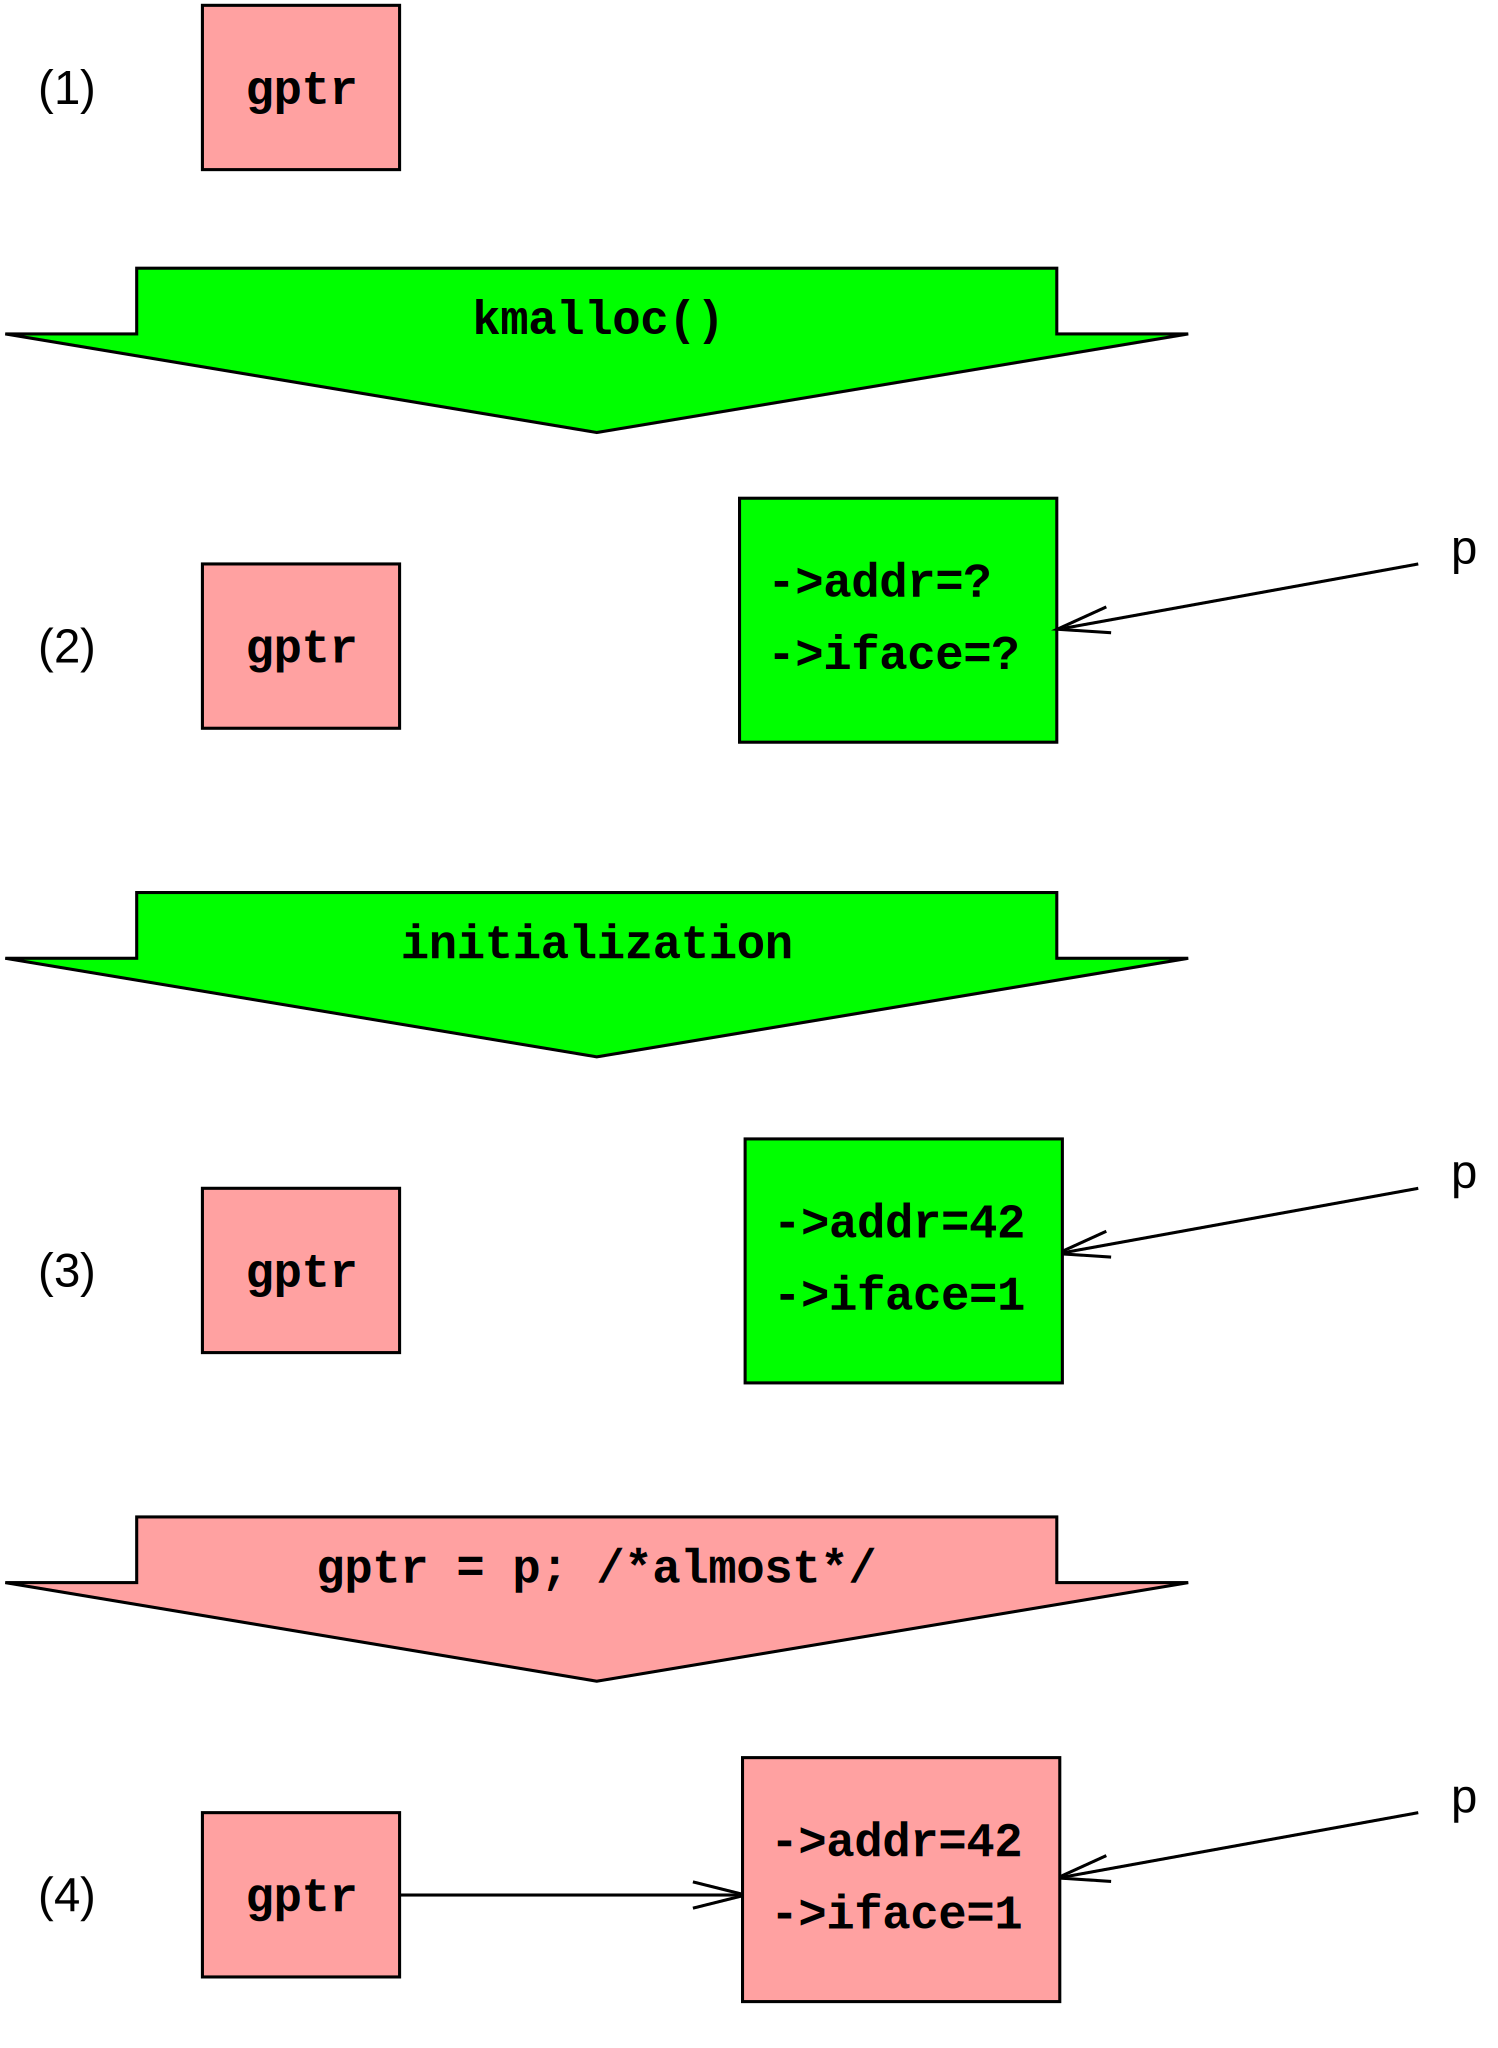
\includegraphics{defer/RCUListInsertClassic}}
\caption{Insertion With Concurrent Readers}
\label{fig:defer:Insertion With Concurrent Readers}
\end{figure}

To minimize implementability concerns, we focus on a minimal
data structure, which consists of a single global pointer that is either
\co{NULL} or references a single structure.
Minimal though it might be, this data structure is heavily used in
production~\cite{GeoffRomer2018C++DeferredReclamationP0561R4}.
A classic approach for insertion is shown in
Figure~\ref{fig:defer:Insertion With Concurrent Readers},
which shows four states with time advancing from top to bottom.
The first row shows the initial state, with \co{gptr} equal to \co{NULL}.
In the second row, we have allocated a structure which is uninitialized,
as indicated by the question marks.
In the third row, we have initialized the structure.
Finally, in the fourth and final row, we have updated \co{gptr} to
reference the newly allocated and initialized element.

We might hope that this assignment to \co{gptr} could use a simple
C-language assignment statement.
Unfortunately,
Section~\ref{sec:toolsoftrade:Shared-Variable Shenanigans}
dashes these hopes.
Therefore, the updater cannot use a simple C-language assignment, but
must instead use \co{smp_store_release()} as shown in the figure,
or, as will be seen, \co{rcu_assign_pointer()}.

Similarly, one might hope that readers could use a single C-language
assignment to fetch the value of \co{gptr}, and be guaranteed to either
get the old value of \co{NULL} or to get the newly installed pointer,
but either way see a valid result.
Unfortunately, Section~\ref{sec:toolsoftrade:Shared-Variable Shenanigans}
dashes these hopes as well.
To obtain this guarantee, readers must instead use \co{READ_ONCE()},
or, as will be seen, \co{rcu_dereference()}.
However, on most modern computer systems, each of these read-side primitives
can be implemented with a single load instruction, exactly the instruction
that would normally be used in single-threaded code.

Reviewing \cref{fig:defer:Insertion With Concurrent Readers}
from the viewpoint of readers, in the first three states all readers
see \co{gptr} having the value \co{NULL}.
Upon entering the fourth state, some readers might see \co{gptr} still
having the value \co{NULL} while others might see it referencing the
newly inserted element, but after some time, all readers will see this
new element.
At all times, all readers will see \co{gptr} as containing a valid pointer.
Therefore, it really is possible to add new data to linked data structures
while allowing concurrent readers to execute the same sequence of machine
instructions that is normally used in single-threaded code.
This no-cost approach to concurrent reading provides excellent performance
and scalability, and also is eminently suitable for real-time use.

\begin{figure}[tb]
\centering
\resizebox{3in}{!}{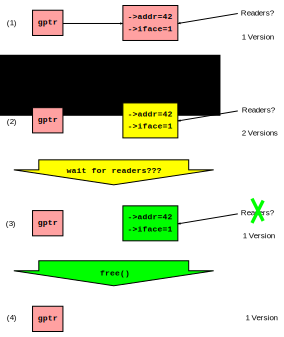
\includegraphics{defer/RCUListDeleteClassic}}
\caption{Deletion With Concurrent Readers}
\label{fig:defer:Deletion With Concurrent Readers}
\end{figure}

Insertion is of course quite useful, but sooner or later, it will also
be necessary to delete data.
As can be seen in
Figure~\ref{fig:defer:Deletion With Concurrent Readers},
the first step is easy.
Again taking the lessons from
Section~\ref{sec:toolsoftrade:Shared-Variable Shenanigans}
to heart, \co{smp_store_release()} is used to \co{NULL} the pointer,
thus moving from the first row to the second in the figure.
At this point, pre-existing readers see the old structure with
\co{->addr} of 42 and \co{->iface} of 1, but new readers will see
a \co{NULL} pointer, that is, concurrent readers can disagree on
the state, as indicated by the ``2 Versions'' in the figure.

\QuickQuizSeries{%
\QuickQuizB{
	Why does
	Figure~\ref{fig:defer:Deletion With Concurrent Readers}
	use \co{smp_store_release()} given that it is storing
	a \co{NULL} pointer?
	Wouldn't \co{WRITE_ONCE()} work just as well in this case,
	given that there is no structure initialization to order
	against the store of the \co{NULL} pointer?
}\QuickQuizAnswerB{
	Yes, it would.

	Because a \co{NULL} pointer is being assigned, there is nothing
	to order against, so there is no need for \co{smp_store_release()}.
	In contrast, when assigning a non-\co{NULL} pointer, it is
	necessary to use \co{smp_store_release()} in order to ensure
	that initialization of the pointed-to structure is carried
	out before assignment of the pointer.

	In short, \co{WRITE_ONCE()} would work, and would
	save a little bit of CPU time on some architectures.
	However, as we will see, software-engineering concerns
	will motivate use of a special \co{rcu_assign_pointer()}
	that is quite similar to \co{smp_store_release()}.
}\QuickQuizEndB
%
\QuickQuizE{
	Readers running concurrently each other and with the procedure
	outlined in
	Figure~\ref{fig:defer:Deletion With Concurrent Readers}
	can disagree on the value of \co{gptr}.
	Isn't that just a wee bit problematic???
}\QuickQuizAnswerE{
	Not necessarily.

	As hinted at in Sections~\ref{sec:cpu:Hardware Optimizations}
	and~\ref{sec:cpu:Hardware Free Lunch?},
	speed-of-light delays mean that a computer's data is always
	stale compared to whatever external reality that data is intended
	to model.

	Real-world algorithms therefore absolutely must tolerate
	inconsistancies between external reality and the in-computer
	data reflecting that reality.
	Many of those algorithms are also able to tolerate some degree
	of inconsistency within the in-computer data.
	Section~\ref{sec:datastruct:RCU-Protected Hash Table Discussion}
	discusses this point in more detail.

	Please note that this need to tolerate inconsistent and stale
	data is not limited to RCU\@.
	It also applies to reference counting, hazard pointers, sequence
	locks, and even to some locking use cases.
	For example, if you compute some quantity while holding a lock,
	but use that quantity after releasing that lock,
	you might well be using stale data.
	After all, the data that quantity is based on might change
	arbitrarily as soon as the lock is released.

	So yes, RCU readers can see stale and inconsistent data, but no,
	this is not necessarily problematic.
	And, when needed, there are RCU usage patterns that avoid both
	staleness and inconsistency~\cite{Arcangeli03}.
}\QuickQuizEndE
}

We get back to a single version simply by waiting for all the
pre-existing readers to complete, as shown in row~3.
At that point, all the pre-existing readers are done, and no later
reader has a path to the old data item, so there can no longer be
any readers referencing it.
It may therefore be safely freed, as shown on row~4.

Thus, given a way to wait for pre-existing readers to complete,
it is possible to both add data to and remove data from a linked
data structure, despite the readers executing the same sequence
of machine instructions that would be appropriate for single-threaded
execution.
So perhaps going all the way was not too far after all!

But how can we tell when all of the pre-existing readers have in
fact completed?
This question is the topic of the next section.

\subsubsection{Waiting for Readers}
\label{sec:defer:Waiting for Readers}

It is tempting to base reader waiting on reference counting, but
Figure~\ref{fig:count:Atomic Increment Scalability on x86}
in
Chapter~\ref{chp:Counting}
shows that concurrent reference counting results in extreme overhead,
as we already saw in
Section~\ref{sec:defer:Reference Counting}.
Hazard pointers profoundly reduce this overhead, but, as we saw in
Section~\ref{sec:defer:Hazard Pointers}, not to zero.
Nevertheless, many RCU implementations make very careful cache-local
use of counters.

A second approach observes that memory synchronization is expensive,
and therefore uses registers instead, namely each CPU's or thread's
program counter (PC), thus imposing no overhead on readers, at least
in the absence of concurrent updates.
The updater polls each relevant PC, and if that PC is not within read-side
code, then the corresponding CPU or thread is within a quiescent state,
in turn signaling the completion of any reader that might have access
to the newly removed data element.
Once all CPU's or thread's PCs have been observed to be outside of any
reader, the grace period has completed.
Please note that this approach poses some serious challenges, including
memory ordering, functions that are \emph{sometimes} invoked from readers,
and ever-exciting code-motion optimizations.
Nevertheless, this approach is said to be used in
production~\cite{MikeAsh2015Apple}.

A third approach is to simply wait for a fixed period of time that is
long enough to comfortably exceed the lifetime of any reasonable
reader~\cite{Jacobson93,AjuJohn95}.
This can work quite well in hard real-time systems~\cite{YuxinRen2018RTRCU},
but in less exotic
settings, Murphy says that it is critically important to be prepared
even for unreasonably long-lived readers.
To see this, consider the consequences of failing do so:
A data item will be freed while the unreasonable reader is still
referencing it, and that item might well be immediately reallocated,
possibly even as a data item of some other type.
The unreasonable reader and the unwitting reallocator would then
be attempting to use the same memory for two very different purposes.
The ensuing mess will at best be exceedingly difficult to debug.

A fourth approach is to wait forever, secure in the knowledge that
doing so will accommodate even the most unreasonable reader.
This approach is also called ``leaking memory'', and has a bad reputation
due to the fact that memory leaks often require untimely and
inconvenient reboots.
Nevertheless, this is a viable strategy when the update rate and the
uptime are both sharply bounded.
For example, this approach could work well in a high-availability
cluster where systems were periodically crashed in order to ensure
that cluster really remained highly available.\footnote{
	The program that forces the periodic crashing is sometimes
	known as a ``chaos monkey'':
	\url{https://netflix.github.io/chaosmonkey/}.
	However, it might also be a mistake to neglect chaos caused
	by systems running for too long.}
Leaking the memory is also a viable strategy in environments having
garbage collectors, in which case the garbage collector can be thought
of as plugging the leak~\cite{Kung80}.
However, if your environment lacks a garbage collector, read on!

A fifth approach avoids the period crashes in favor of periodically
``stopping the world'', as exemplified by the traditional stop-the-world
garbage collector.
This approach was also heavily used during the decades before
ubiquitous connectivity, when it was common practice to power systems
off at the end of each working day.
However, in today's always-connected always-on world, stopping the world
can gravely degrade response times, which has been one motivation for the
development of concurrent garbage collectors~\cite{DavidFBacon2003RTGC}.
Furthermore, although we need all pre-existing readers to complete, we do
not need them all to complete at the same time.

This observation leads to the sixth approach, which is stopping
one CPU or thread at a time.
This approach has the advantage of not degrading reader response times
at all, let alone gravely.
Furthermore, numerous applications already have states (termed
\emph{quiescent states}) that can be
reached only after all pre-existing readers are done.
In transaction-processing systems, the time between a pair of
successive transactions might be a quiescent state.
In reactive systems, the state between a pair of successive events
might be a quiescent state.
Within non-preemptive operating-systems kernels, a context switch can be
a quiescent state~\cite{McKenney98}.
Either way, once all CPUs and/or threads have passed through a quiescent
state, the system is said to have completed a \emph{grace period},
at which point all readers in existence at the start of that grace period
are guaranteed to have completed.
As a result, it is also guaranteed to be safe to free any removed data
items that were removed prior to the start of that grace period.\footnote{
	It is possible to do much more with RCU than simply defer
	reclamation of memory, but deferred reclamation is RCU's most
	common use case, and is therefore an excellent place to start.}

Within a non-preemptive operating-system kernel, for context switch to be
a valid quiescent state, readers must be prohibited from blocking while
referencing a given instance data structure obtained via the \co{gptr}
pointer shown in
Figures~\ref{fig:defer:Insertion With Concurrent Readers}
and~\ref{fig:defer:Deletion With Concurrent Readers}.
This no-blocking constraint is consistent with similar constraints
on pure spinlocks, where a CPU is forbidden from blocking while
holding a spinlock.
Without this constraint, all CPUs might be consumed by threads
spinning attempting to acquire a spinlock held by a blocked thread.
The spinning threads will not relinquish their CPUs until they acquire
the lock, but the thread holding the lock cannot possibly release it
until one of the spinning threads relinquishes a CPU\@.
This is a classic deadlock situation, and this deadlock is avoided
by forbidding blocking while holding a spinlock.

Again, this same constraint is imposed on reader threads dereferencing
\co{gptr}: such threads are not allowed to block until after
they are done using the pointed-to data item.
Returning to the second row of
Figure~\ref{fig:defer:Deletion With Concurrent Readers},
where the updater has just completed executing the \co{smp_store_release()},
imagine that CPU~0 executes a context switch.
Because readers are not permitted to block while traversing the linked
list, we are guaranteed that all prior readers that might have been running on
CPU~0 will have completed.
Extending this line of reasoning to the other CPUs, once each CPU has
been observed executing a context switch, we are guaranteed that all
prior readers have completed, and that there are no longer any reader
threads referencing the newly removed data element.
The updater can then safely free that data element, resulting in the
state shown at the bottom of
Figure~\ref{fig:defer:Deletion With Concurrent Readers}.

\begin{figure}[tb]
\centering
\resizebox{3in}{!}{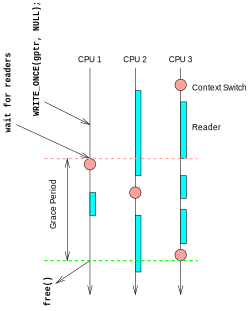
\includegraphics{defer/QSBRGracePeriod}}
\caption{QSBR: Waiting for Pre-Existing Readers}
\label{fig:defer:QSBR: Waiting for Pre-Existing Readers}
\end{figure}

This approach is termed \emph{quiescent state based reclamation}
(QSBR)~\cite{ThomasEHart2006a}.
A QSBR schematic is shown in
Figure~\ref{fig:defer:QSBR: Waiting for Pre-Existing Readers},
with time advancing from the top of the figure to the bottom.
CPU~1 does the \co{WRITE_ONCE()} that removes the current data
item (presumably having previously read the pointer value and
availed itself of appropriate synchronization), then waits
for readers.
This wait operation results in an immediate context switch, which is a
quiescent state (denoted by the pink circle), which in turn means that
all prior reads on CPU~1 have completed.
Next, CPU~2 does a context switch, so that all readers on CPUs~1 and~2
are now known to have completed.
Finally, CPU~3 does a context switch.
At this point, all readers throughout the entire system are known to
have completed, so the grace period ends, permitting CPU~1 to free
the old data item.

\QuickQuiz{
	In Figure~\ref{fig:defer:QSBR: Waiting for Pre-Existing Readers},
	the last of CPU~3's readers that could possibly have
	access to the old data item ended before the grace period
	even started!
	So why would anyone bother waiting until CPU~3's later context
	switch???
}\QuickQuizAnswer{
	Because that waiting is exactly what enables readers to use
	the same sequence of instructions that is appropriate for
	single-theaded situations.
	In other words, this additional ``redundant'' waiting enables
	excellent read-side performance, scalability, and real-time
	response.
}\QuickQuizEnd

\subsubsection{Toy Implementation}
\label{sec:defer:Toy Implementation}

Although production-quality QSBR implementations can be quite complex,
a toy non-preemptive Linux-kernel implementation is exceedingly simple:

\begin{VerbatimN}[samepage=true]
void synchronize_rcu(void)
{
	int cpu;

	for_each_online_cpu(cpu)
		sched_setaffinity(current->pid, cpumask_of(cpu));
}
\end{VerbatimN}

The \co{for_each_online_cpu()} primitive iterates over all CPUs, and
the \co{sched_setaffinity()} function causes the current thread to
execute on the specified CPU, which forces the destination CPU to execute
a context switch.
Therefore, once the \co{for_each_online_cpu()} has completed, each CPU
has executed a context switch, which in turn guarantees that
all pre-existing reader threads have completed.

\begin{listing}[tbp]
\begin{fcvlabel}[ln:defer:Insertion and Deletion With Concurrent Readers]
\begin{VerbatimL}[commandchars=\\\[\]]
struct route *gptr;

int access_route(int (*f)(struct route *rp))
{
	int ret = -1;
	struct route *rp;

	rcu_read_lock();
	rp = rcu_dereference(gptr);
	if (rp)
		ret = f(rp);		\lnlbl[access_rp]
	rcu_read_unlock();
	return ret;
}

struct route *ins_route(struct route *rp)
{
	struct route *old_rp;

	spin_lock(&route_lock);
	old_rp = gptr;
	rcu_assign_pointer(gptr, rp);
	spin_unlock(&route_lock);
	return old_rp;
}

int del_route(void)
{
	struct route *old_rp;

	spin_lock(&route_lock);
	old_rp = gptr;
	RCU_INIT_POINTER(gptr, NULL);
	spin_unlock(&route_lock);
	synchronize_rcu();
	free(old_rp);
	return !!old_rp;
}
\end{VerbatimL}
\end{fcvlabel}
\caption{Insertion and Deletion With Concurrent Readers}
\label{lst:defer:Insertion and Deletion With Concurrent Readers}
\end{listing}

Please note that this approach is \emph{not} production quality.
Correct handling of a number of corner cases and the need for a number
of powerful optimizations mean that production-quality implementations
are quite complex.
In addition, RCU implementations for preemptible environments
require that readers actually do something, which in non-real-time
Linux-kernel environments can be as simple as defining
\co{rcu_read_lock()} and \co{rcu_read_unlock()} as \co{preempt_disable()}
and \co{preempt_enable()}, respectively.\footnote{
	Some toy RCU implementations that handle preempted
	read-side critical sections are shown in
	Appendix~\ref{chp:app:``Toy'' RCU Implementations}.}
However, this simple non-preemptible approach is conceptually complete,
and demonstrates that it really is possible to provide read-side
synchronization at zero cost, even in the face of concurrent updates.
In fact,
Listing~\ref{lst:defer:Insertion and Deletion With Concurrent Readers}
shows how reading (\co{access_route()}),
Figure~\ref{fig:defer:Insertion With Concurrent Readers}'s
insertion (\co{ins_route()}) and
Figure~\ref{fig:defer:Deletion With Concurrent Readers}'s
deletion (\co{del_route()}) can
be implemented.
(A slightly more capable routing table is shown in
Section~\ref{sec:defer:RCU for Pre-BSD Routing}.)

\QuickQuizSeries{%
\QuickQuizB{
	What is the point of \co{rcu_read_lock()} and \co{rcu_read_unlock()} in
	Listing~\ref{lst:defer:Insertion and Deletion With Concurrent Readers}?
	Why not just let the quiescent states speak for themselves?
}\QuickQuizAnswerB{
	Recall that readers are not permitted to pass through a quiescent
	state.
	For example, within the Linux kernel, RCU readers are not permitted
	to execute a context switch.
	Use of \co{rcu_read_lock()} and \co{rcu_read_unlock()} enables
	debug checks for improperly placed quiescent states, making it
	easy to find bugs that would otherwise be difficult to find,
	intermittent, and quite destructive.
}\QuickQuizEndB
%
\QuickQuizE{
	What is the point of \co{rcu_dereference()}, \co{rcu_assign_pointer()}
	and \co{RCU_INIT_POINTER()} in
	Listing~\ref{lst:defer:Insertion and Deletion With Concurrent Readers}?
	Why not just use \co{READ_ONCE()}, \co{smp_store_release()}, and
	\co{WRITE_ONCE()}, respectively?
}\QuickQuizAnswerE{
	The RCU-specific APIs do have similar semantics to the suggested
	replacements, but also enable static-analysis debugging checks
	that complain if an RCU-specific API is invoked on a non-RCU
	pointer and vice versa.
}\QuickQuizEndE
}

Referring back to
Listing~\ref{lst:defer:Insertion and Deletion With Concurrent Readers},
note that \co{route_lock} is used to synchronize between concurrent updaters
invoking \co{ins_route()} and \co{del_route()}.
However, this lock is not acquired by readers invoking \co{access_route()}:
Readers are instead protected by the QSBR techniques described in this section.

Note that \co{ins_route()} simply returns the old value of \co{gptr}, which
Figure~\ref{fig:defer:Insertion With Concurrent Readers} assumed would
always be \co{NULL}.
This means that it is the caller's responsibility to figure out what to
do with a non-\co{NULL} value, a task complicated by the fact that
readers might still be referencing it for an indeterminate period of time.
Callers might use one of the following approaches:

\begin{enumerate}
\item	Use \co{synchronize_rcu()} to safely free the pointed-to structure.
	Although this approach is correct from an RCU perspective, it
	arguably has software-engineering leaky-API problems.
\item	Trip an assertion if the returned pointer is non-\co{NULL}.
\item	Pass the returned pointer to a later invocation of
	\co{ins_route()} to restore the earlier value.
\end{enumerate}

In contrast, \co{del_route()} uses \co{synchronize_rcu()} and
\co{free()} to safely free the newly deleted data item.

\QuickQuiz{
	But what if the old structure needs to be freed, but the caller
	of \co{ins_route()} cannot block, perhaps due to performance
	considerations or perhaps because the caller is executing within
	an RCU read-side critical section?
}\QuickQuizAnswer{
	A \co{call_rcu()} function, which is described in
	Section~\ref{sec:defer:Wait For Pre-Existing RCU Readers},
	permits asynchronous grace-period waits.
}\QuickQuizEnd

This example shows one general approach to reading and updating
RCU-protected data structures, however, there is quite a variety
of use cases, several of which are covered in
Section~\ref{sec:defer:RCU Usage}.

In summary, it is in fact possible to create concurrent linked data
structures that can be traversed by readers executing the same sequence
of machine instructions that would be executed by single-threaded readers.
The next section summarizes RCU's high-level properties.

\subsubsection{RCU Properties}
\label{sec:defer:RCU Properties}

A key RCU property is that reads need not wait for updates.
This property enables RCU implementations to provide low-cost or even
no-cost readers, resulting in low overhead and excellent scalability.
This property also allows RCU readers and updaters to make useful
concurrent forward progress.
In contrast, conventional synchronization primitives must enforce strict
mutual exclusion using expensive instructions, thus increasing overhead
and degrading scalability, but also typically prohibiting readers and
updaters from making useful concurrent forward progress.

\QuickQuiz{
	Doesn't Section~\ref{sec:defer:Sequence Locks}'s seqlock
	also permit readers and updaters to make useful concurrent
	forward progress?
}\QuickQuizAnswer{
	Yes and no.
	Although seqlock readers can run concurrently with
	seqlock writers, whenever this happens, the \co{read_seqretry()}
	primitive will force the reader to retry.
	This means that any work done by a seqlock reader running concurrently
	with a seqlock updater will be discarded and the redone upon retry.
	So seqlock readers can \emph{run} concurrently with updaters,
	but they cannot actually get any work done in this case.

	In contrast, RCU readers can perform useful work even in presence
	of concurrent RCU updaters.

	However, both reference counters
	(Section~\ref{sec:defer:Reference Counting})
	and hazard pointers
	(Section~\ref{sec:defer:Hazard Pointers})
	really do permit useful concurrent forward progress for both
	updaters and readers, just at somewhat greater cost.
	Please see
	Section~\ref{sec:defer:Which to Choose?}
	for a comparison of these different solutions to the
	deferred-reclamation problem.
}\QuickQuizEnd

RCU delimits readers with \co{rcu_read_lock()} and \co{rcu_read_unlock()},
and ensures that each reader has a coherent view of each object
(see \cref{fig:defer:Deletion With Concurrent Readers}) by
maintaining multiple versions of objects and using update-side primitives
such as \co{synchronize_rcu()} to ensure that objects are not
freed until after the completion of all readers that might be using them.
RCU uses \co{rcu_assign_pointer()} and \co{rcu_dereference()} to provide
efficient and scalable mechanisms for publishing and reading new versions
of an object, respectively.
These mechanisms distribute the work among read and
update paths in such a way as to make read paths extremely fast, using
replication and weakening optimizations in a manner similar to
hazard pointers, but without the need for read-side retries.
In some cases, including \co{CONFIG_PREEMPT=n} Linux kernels,
RCU's read-side primitives have zero overhead.

But are these properties actually useful in practice?
This question is taken up by the next section.

\subsubsection{Practical Applicability}
\label{sec:defer:Practical Applicability}

\begin{figure}[tb]
\centering
\resizebox{3in}{!}{\includegraphics{defer/linux-RCU}}
\caption{RCU Usage in the Linux Kernel}
\label{fig:defer:RCU Usage in the Linux Kernel}
\end{figure}

RCU has been used in the Linux kernel since
October 2002~\cite{Torvalds2.5.43}.
Use of the RCU API has increased substantially since that time,
as can be seen in
Figure~\ref{fig:defer:RCU Usage in the Linux Kernel}.
In fact, code very similar to that in
Listing~\ref{lst:defer:Insertion and Deletion With Concurrent Readers}
is used in the Linux kernel.
RCU has enjoyed heavy use both prior to and since its acceptance
in the Linux kernel, as discussed in
\cref{sec:defer:RCU Related Work}.

It is therefore safe to say that RCU enjoys wide practical applicability.

The minimal example discussed in this section is a good introduction to RCU\@.
However, effective use of RCU often requires that you think differently
about your problem.
It is therefore useful to examine RCU's fundamentals, a task taken up
by the following section.

% defer/rcufundamental.tex

\subsection{RCU Fundamentals}
\label{sec:defer:RCU Fundamentals}
\OriginallyPublished{Section}{sec:defer:RCU Fundamentals}{RCU Fundamentals}{Linux Weekly News}{PaulEMcKenney2007WhatIsRCUFundamentally}

RCU is made up of three fundamental mechanisms, the first being
used for insertion, the second being used for deletion, and the third
being used to allow readers to tolerate concurrent insertions and deletions.
Section~\ref{sec:defer:Publish-Subscribe Mechanism}
describes the publish-subscribe mechanism used for insertion,
Section~\ref{sec:defer:Wait For Pre-Existing RCU Readers}
describes how waiting for pre-existing RCU readers enabled deletion,
and
Section~\ref{sec:defer:Maintain Multiple Versions of Recently Updated Objects}
discusses how maintaining multiple versions of recently updated objects
permits concurrent insertions and deletions.
Finally,
Section~\ref{sec:defer:Summary of RCU Fundamentals}
summarizes RCU fundamentals.

\subsubsection{Publish-Subscribe Mechanism}
\label{sec:defer:Publish-Subscribe Mechanism}

% @@@ Slim down presentation, refer to toolsoftrade and memorder.
% @@@ Summarize care and feeding of address dependencies.
% @@@ Mention language/compiler support being a work in progress.

\begin{listing}[tbp]
\begin{VerbatimL}
struct foo {
	int a;
	int b;
	int c;
};
struct foo *gp = NULL;

/* . . . */

p = kmalloc(sizeof(*p), GFP_KERNEL);
p->a = 1;
p->b = 2;
p->c = 3;
gp = p;
\end{VerbatimL}
\caption{Data Structure Publication (Unsafe)}
\label{lst:defer:Data Structure Publication (Unsafe)}
\end{listing}

One key attribute of RCU is the ability to safely scan data, even
though that data is being modified concurrently.
To provide this ability for concurrent insertion,
RCU uses what can be thought of as a publish-subscribe mechanism.
For example, consider an initially \co{NULL} global pointer
\co{gp} that is to be modified to point to a newly allocated
and initialized data structure.
The code fragment shown in
Listing~\ref{lst:defer:Data Structure Publication (Unsafe)}
(with the addition of appropriate locking)
might be used for this purpose.

Unfortunately, there is nothing forcing the compiler and CPU to execute
the last four assignment statements in order.
If the assignment to \co{gp} happens before the initialization
of \co{p} fields, then concurrent readers could see the
uninitialized values.
Memory barriers are required to keep things ordered, but memory barriers
are notoriously difficult to use.
We therefore encapsulate them into a primitive
\co{rcu_assign_pointer()} that has publication semantics.
The last four lines would then be as follows:

\begin{VerbatimN}[samepage=true]
p->a = 1;
p->b = 2;
p->c = 3;
rcu_assign_pointer(gp, p);
\end{VerbatimN}

The \co{rcu_assign_pointer()}
would \emph{publish} the new structure, forcing both the compiler
and the CPU to execute the assignment to \co{gp} \emph{after}
the assignments to the fields referenced by \co{p}.

However, it is not sufficient to only enforce ordering at the
updater, as the reader must enforce proper ordering as well.
Consider for example the following code fragment:

\begin{VerbatimN}[samepage=true]
p = gp;
if (p != NULL) {
	do_something_with(p->a, p->b, p->c);
}
\end{VerbatimN}

Although this code fragment might well seem immune to misordering,
unfortunately, the
DEC Alpha CPU~\cite{PaulMcKenney2005i,PaulMcKenney2005j}
and value-speculation compiler optimizations can, believe it or not,
cause the values of \co{p->a}, \co{p->b}, and
\co{p->c} to be fetched before the value of \co{p}.
This is perhaps easiest to see in the case of value-speculation
compiler optimizations, where the compiler guesses the value
of \co{p}, fetches \co{p->a}, \co{p->b}, and
\co{p->c}, and then fetches the actual value of \co{p}
in order to check whether its guess was correct.
This sort of optimization is quite aggressive, perhaps insanely so,
but does actually occur in the context of profile-driven optimization.

Clearly, we need to prevent this sort of skullduggery on the
part of both the compiler and the CPU.
The \co{rcu_dereference()} primitive uses
whatever memory-barrier instructions and compiler
directives are required for this purpose:\footnote{
	In the Linux kernel, \co{rcu_dereference()} is implemented via
	a volatile cast, and, on DEC Alpha, a memory barrier instruction.
	In the C11 and C++11 standards, \co{memory_order_consume}
	is intended to provide longer-term support for \co{rcu_dereference()},
	but no compilers implement this natively yet.
	(They instead strengthen \co{memory_order_consume} to
	\co{memory_order_acquire}, thus emitting a needless memory-barrier
	instruction on weakly ordered systems.)}

\begin{VerbatimN}[samepage=true]
rcu_read_lock();
p = rcu_dereference(gp);
if (p != NULL) {
	do_something_with(p->a, p->b, p->c);
}
rcu_read_unlock();
\end{VerbatimN}

The \co{rcu_dereference()} primitive can thus be thought of
as \emph{subscribing} to a given value of the specified pointer,
guaranteeing that subsequent dereference operations will see any
initialization that occurred before the corresponding
\co{rcu_assign_pointer()} operation that published that pointer.
The \co{rcu_read_lock()} and \co{rcu_read_unlock()}
calls are absolutely required: they define the extent of the
RCU read-side critical section.
Their purpose is explained in
Section~\ref{sec:defer:Wait For Pre-Existing RCU Readers},
however, they never spin or block, nor do they prevent the
\co{list_add_rcu()} from executing concurrently.
In fact, in non-\co{CONFIG_PREEMPT} kernels, they generate
absolutely no code.

\begin{figure}[tb]
\centering
\resizebox{3in}{!}{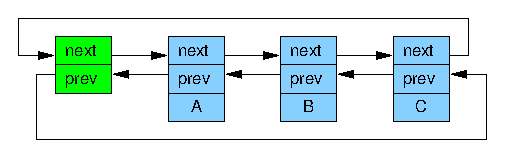
\includegraphics{defer/Linux_list}}
\caption{Linux Circular Linked List}
\label{fig:defer:Linux Circular Linked List}
\end{figure}

\begin{figure}[tb]
\centering
\resizebox{1.8in}{!}{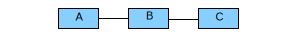
\includegraphics{defer/Linux_list_abbr}}
\caption{Linux Linked List Abbreviated}
\label{fig:defer:Linux Linked List Abbreviated}
\end{figure}

Although \co{rcu_assign_pointer()} and
\co{rcu_dereference()} can in theory be used to construct any
conceivable RCU-protected data structure, in practice it is often better
to use higher-level constructs.
Therefore, the \co{rcu_assign_pointer()} and
\co{rcu_dereference()}
primitives have been embedded in special RCU variants of Linux's
list-manipulation API.
Linux has two variants of doubly linked list, the circular
\co{struct list_head} and the linear
\co{struct hlist_head}/\co{struct hlist_node} pair.
The former is laid out as shown in
Figure~\ref{fig:defer:Linux Circular Linked List},
where the green (leftmost) boxes represent the list header and the blue
(rightmost three) boxes represent the elements in the list.
This notation is cumbersome, and will therefore be abbreviated as shown in
Figure~\ref{fig:defer:Linux Linked List Abbreviated},
which shows only the non-header (blue) elements.

\begin{listing}[tbp]
\begin{linelabel}[ln:defer:RCU Data Structure Publication]
\begin{VerbatimL}[commandchars=\\\[\]]
struct foo {
	struct list_head *list;
	int a;
	int b;
	int c;
};
LIST_HEAD(head);

/* . . . */

p = kmalloc(sizeof(*p), GFP_KERNEL);
p->a = 1;
p->b = 2;
p->c = 3;
list_add_rcu(&p->list, &head);		\lnlbl[add_rcu]
\end{VerbatimL}
\end{linelabel}
\caption{RCU Data Structure Publication}
\label{lst:defer:RCU Data Structure Publication}
\end{listing}

Adapting the pointer-publish example for the linked list results in
the code shown in
Listing~\ref{lst:defer:RCU Data Structure Publication}.

Line~\ref{ln:defer:RCU Data Structure Publication:add_rcu}
must be protected by some synchronization mechanism (most
commonly some sort of lock) to prevent multiple \co{list_add_rcu()}
instances from executing concurrently.
However, such synchronization does not prevent this \co{list_add()}
instance from executing concurrently with RCU readers.

Subscribing to an RCU-protected list is straightforward:

\begin{VerbatimN}[samepage=true]
rcu_read_lock();
list_for_each_entry_rcu(p, head, list) {
	do_something_with(p->a, p->b, p->c);
}
rcu_read_unlock();
\end{VerbatimN}

The \co{list_add_rcu()} primitive publishes an entry, inserting it at
the head of the specified list, guaranteeing that the corresponding
\co{list_for_each_entry_rcu()} invocation will properly subscribe to
this same entry.

\QuickQuiz{}
	What prevents the \co{list_for_each_entry_rcu()} from
	getting a segfault if it happens to execute at exactly the same
	time as the \co{list_add_rcu()}?
\QuickQuizAnswer{
	On all systems running Linux, loads from and stores
	to pointers are atomic, that is, if a store to a pointer occurs at
	the same time as a load from that same pointer, the load will return
	either the initial value or the value stored, never some bitwise
	mashup of the two.
	In addition, the \co{list_for_each_entry_rcu()} always proceeds
	forward through the list, never looking back.
	Therefore, the \co{list_for_each_entry_rcu()} will either see
	the element being added by \co{list_add_rcu()} or it will not,
	but either way, it will see a valid well-formed list.
} \QuickQuizEnd

\begin{figure}[tb]
\centering
\resizebox{3in}{!}{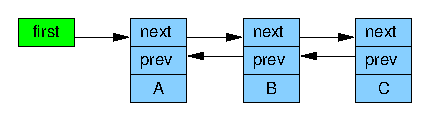
\includegraphics{defer/Linux_hlist}}
\caption{Linux Linear Linked List}
\label{fig:defer:Linux Linear Linked List}
\end{figure}

Linux's other doubly linked list, the hlist,
is a linear list, which means that
it needs only one pointer for the header rather than the two
required for the circular list, as shown in
Figure~\ref{fig:defer:Linux Linear Linked List}.
Thus, use of hlist can halve the memory consumption for the hash-bucket
arrays of large hash tables.
As before, this notation is cumbersome, so hlists will be abbreviated
in the same way lists are, as shown in
Figure~\ref{fig:defer:Linux Linked List Abbreviated}.

\begin{listing}[tbp]
\begin{linelabel}[ln:defer:RCU hlist Publication]
\begin{VerbatimL}[commandchars=\\\[\]]
struct foo {
	struct hlist_node *list;
	int a;
	int b;
	int c;
};
HLIST_HEAD(head);

/* . . . */

p = kmalloc(sizeof(*p), GFP_KERNEL);
p->a = 1;
p->b = 2;
p->c = 3;
hlist_add_head_rcu(&p->list, &head);	\lnlbl[add_head]
\end{VerbatimL}
\end{linelabel}
\caption{RCU {\tt hlist} Publication}
\label{lst:defer:RCU hlist Publication}
\end{listing}

Publishing a new element to an RCU-protected hlist is quite similar
to doing so for the circular list,
as shown in Listing~\ref{lst:defer:RCU hlist Publication}.

As before, line~\ref{ln:defer:RCU hlist Publication:add_head}
must be protected by some sort of synchronization
mechanism, for example, a lock.

Subscribing to an RCU-protected hlist is also similar to the
circular list:

\begin{VerbatimN}[samepage=true]
rcu_read_lock();
hlist_for_each_entry_rcu(p, head, list) {
	do_something_with(p->a, p->b, p->c);
}
rcu_read_unlock();
\end{VerbatimN}

\begin{table*}[tb]
\renewcommand*{\arraystretch}{1.2}
\centering
\footnotesize\OneColumnHSpace{-0.4in}
\begin{tabular}{llll}
\toprule
Category  & Publish	& Retract	& Subscribe \\
\midrule
Pointers  & \tco{rcu_assign_pointer()}
			& \tco{rcu_assign_pointer(..., NULL)}
					& \tco{rcu_dereference()} \\
\midrule
Lists     & \parbox[c][0.37in][c]{1.3in}{
		\co{list_add_rcu()} \\
		\co{list_add_tail_rcu()} \\
		\co{list_replace_rcu()} }
			& \tco{list_del_rcu()}
					& \tco{list_for_each_entry_rcu()} \\
\midrule
Hlists    & \parbox[c][0.5in][c]{1.3in}{
		\co{hlist_add_behind_rcu()} \\
		\co{hlist_add_before_rcu()} \\
		\co{hlist_add_head_rcu()} \\
		\co{hlist_replace_rcu()} }
			& \tco{hlist_del_rcu()}
					& \tco{hlist_for_each_entry_rcu()} \\
\bottomrule
\end{tabular}
\caption{RCU Publish and Subscribe Primitives}
\label{tab:defer:RCU Publish and Subscribe Primitives}
\end{table*}

The set of RCU publish and subscribe primitives are shown in
Table~\ref{tab:defer:RCU Publish and Subscribe Primitives},
along with additional primitives to ``unpublish'', or retract.

Note that the \co{list_replace_rcu()}, \co{list_del_rcu()},
\co{hlist_replace_rcu()}, and \co{hlist_del_rcu()}
APIs add a complication.
When is it safe to free up the data element that was replaced or
removed?
In particular, how can we possibly know when all the readers
have released their references to that data element?

These questions are addressed in the following section.

\subsubsection{Wait For Pre-Existing RCU Readers}
\label{sec:defer:Wait For Pre-Existing RCU Readers}

In its most basic form, RCU is a way of waiting for things to finish.
Of course, there are a great many other ways of waiting for things to
finish, including reference counts, reader-writer locks, events, and so on.
The great advantage of RCU is that it can wait for each of
(say) 20,000 different things without having to explicitly
track each and every one of them, and without having to worry about
the performance degradation, scalability limitations, complex deadlock
scenarios, and memory-leak hazards that are inherent in schemes
using explicit tracking.

In RCU's case, each of the things waited on is called an
\emph{RCU read-side critical section}.
As hinted at in
Section~\ref{sec:defer:Toy Implementation}, an RCU read-side critical
section starts with an \co{rcu_read_lock()} primitive, and ends with a
corresponding \co{rcu_read_unlock()} primitive.
RCU read-side critical sections can be nested, and may contain pretty
much any code, as long as that code does not contain a quiescent state,
for example, within the Linux kernel, it is illegal to sleep within
an RCU read-side critical section because a context switch is a quiescent
state.\footnote{
	However, a special form of RCU called SRCU~\cite{PaulEMcKenney2006c}
	does permit general sleeping in SRCU read-side critical sections.}
If you abide by these conventions, you can use RCU to wait for \emph{any}
pre-existing RCU read-side critical section to complete, and
\co{synchronize_rcu()} does the actual waiting.

% @@@ citations? @@@ RCU accomplishes this feat by indirectly determining
% when these other things have finished~\cite{PaulEMcKenney2007whatisRCU,
% PaulEMcKenney2007PreemptibleRCU}.

\begin{figure}[tb]
\centering
\resizebox{3in}{!}{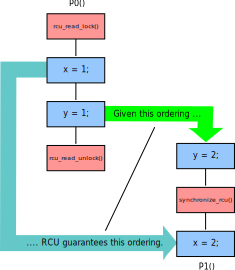
\includegraphics{defer/RCUGuaranteeFwd}}
\caption{RCU Reader and Later Grace Period}
\label{fig:defer:RCU Reader and Later Grace Period}
\end{figure}

The relationship between an RCU read-side critical section and a later
RCU grace period is an if-then relationship, as illustrated by
Figure~\ref{fig:defer:RCU Reader and Later Grace Period}.
If any portion of a given critical section precedes the beginning of
a given grace period, then RCU guarantees that all of that critical
section will precede the end of that grace period.
In the figure, because \co{P0()}'s access to \co{y} precedes
\co{P1()}'s access to this same variable, it is guaranteed that
\co{P0()}'s access to \co{x} will precede \co{P1()}'s access.
In this case, if \co{y}'s final value is 2, then \co{x}'s
final value is guaranteed to also be 2.

\QuickQuiz{}
	What other final values of \co{x} and \co{y} are possible in
	Figure~\ref{fig:defer:RCU Reader and Later Grace Period}?
\QuickQuizAnswer{
	The \co{x == 2 && y == 2} possibility was called out in the text.
	Given that \co{y == 2} implies \co{x == 2}, we know that
	\co{x == 1 && y == 2} is forbidden.
	The following discussion will show that both
	\co{x == 1 && y == 1} and \co{x == 2 && y == 1} are possible.
} \QuickQuizEnd

\begin{figure}[tb]
\centering
\resizebox{3in}{!}{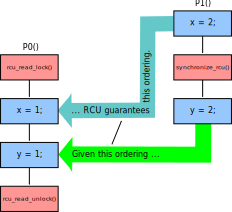
\includegraphics{defer/RCUGuaranteeRev}}
\caption{RCU Reader and Earlier Grace Period}
\label{fig:defer:RCU Reader and Earlier Grace Period}
\end{figure}

The relationship between an RCU read-side critical section and an earlier
RCU grace period is also an if-then relationship, as illustrated by
Figure~\ref{fig:defer:RCU Reader and Earlier Grace Period}.
If any portion of a given critical section follows the end of
a given grace period, then RCU guarantees that all of that critical
section will follow the beginning of that grace period.
In the figure, because \co{P0()}'s access to \co{x} follows
\co{P1()}'s access to this same variable, it is guaranteed that
\co{P0()}'s access to \co{y} will precede \co{P1()}'s access.
In this case, if \co{x}'s final value is 1, then \co{y}'s
final value is guaranteed to also be 1.

\begin{figure}[tb]
\centering
\resizebox{3in}{!}{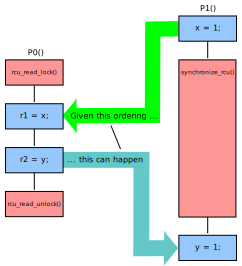
\includegraphics{defer/RCUGuaranteeMid}}
\caption{RCU Reader Within Grace Period}
\label{fig:defer:RCU Reader Within Grace Period}
\end{figure}

Finally, as shown in
Figure~\ref{fig:defer:RCU Reader Within Grace Period},
an RCU read-side critical section can be completely overlapped by
an RCU grace period.
In this case, \co{x}'s final value is 1 and \co{y}'s final value is 2.

However, it cannot be the case that \co{x}'s final value is 2 and \co{y}'s
final value is 1.
This would mean that an RCU read-side critical section had completely
overlapped a grace period, which is forbidden.
RCU's wait-for-readers guarantee therefore has two parts:
(1)~If any part of a given RCU read-side critical section precedes
the beginning of a given grace period, then the entirety of that
critical section precedes the end of that grace period.
(2)~If any part of a given RCU read-side critical section follows
the end of a given grace period, then the entirety of that
critical section follows the beginning of that grace period.
This definition is sufficient for almost all RCU-based algorithms, but
for those wanting more,
simple executable formal models of RCU are available
as part of Linux kernel v4.17 and later, as discussed in
Section~\ref{sec:formal:Axiomatic Approaches and RCU}.
In addition, RCU's ordering properties are examined in much
greater detail in Section~\ref{sec:memorder:RCU}.

Although RCU's wait-for-readers capability really is sometimes used to
order the assignment of values to variables as shown in
Figures~\ref{fig:defer:RCU Reader and Later Grace Period}-\ref{fig:defer:RCU Reader Within Grace Period},
it is more frequently used to safely free data elements removed from
a linked structure, as was done in
Section~\ref{sec:defer:Introduction to RCU}.
The general process is illustrated by the following pseudocode:

\begin{enumerate}
\item	Make a change, for example, remove an element from a linked list.
\item	Wait for all pre-existing RCU read-side critical sections to
	completely finish (for example, by using
	\co{synchronize_rcu()}).
\item	Clean up, for example, free the element that was replaced above.
\end{enumerate}

Given that RCU readers can make forward progress while this update
is in progress, different readers might disagree about the state
of the data structure, a topic taken up by the next section.

\subsubsection{Maintain Multiple Versions of Recently Updated Objects}
\label{sec:defer:Maintain Multiple Versions of Recently Updated Objects}

This section demonstrates how RCU maintains multiple versions of
lists to accommodate synchronization-free readers.
Two examples are presented showing how an element
that might be referenced by a given reader must remain intact
while that reader remains in its RCU read-side critical section.
The first example demonstrates deletion of a list element,
and the second example demonstrates replacement of an element.

\paragraph{Example 1: Maintaining Multiple Versions During Deletion}
\label{sec:defer:Example 1: Maintaining Multiple Versions During Deletion}

We can now revisit the deletion example from
Section~\ref{sec:defer:Introduction to RCU},
but now with the benefit of a firm understanding of the fundamental
concepts underlying RCU.
% @@@ \begin{lineref}[ln:defer:Canonical RCU Replacement Example]
% @@@ To begin this new version of the deletion example,
% @@@ we will modify
% @@@ lines~\lnref{search}-\lnref{kfree} in
% @@@ Listing~\ref{lst:defer:Canonical RCU Replacement Example}
% @@@ to read as follows:
% @@@ \end{lineref}

\begin{linelabel}[ln:defer:RCU Deletion From Linked List]
\begin{VerbatimN}[samepage=true,commandchars=\\\[\]]
p = search(head, key);
if (p != NULL) {
	list_del_rcu(&p->list);		\lnlbl[del_rcu]
	synchronize_rcu();		\lnlbl[sync_rcu]
	kfree(p);
}
\end{VerbatimN}
\end{linelabel}

\begin{figure}[tb]
\centering
\resizebox{3in}{!}{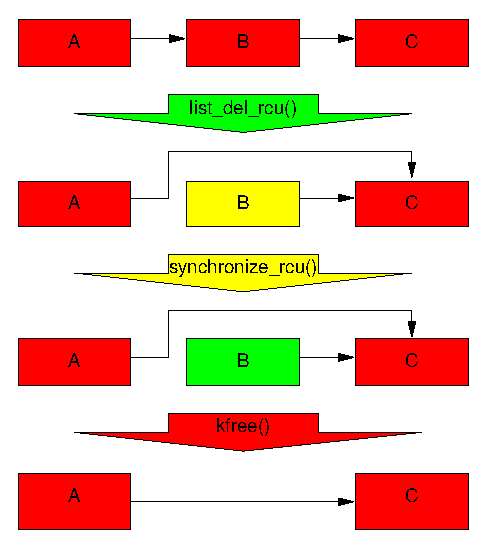
\includegraphics{defer/RCUDeletion}}
\caption{RCU Deletion From Linked List}
\label{fig:defer:RCU Deletion From Linked List}
\end{figure}

This code will update the list as shown in
Figure~\ref{fig:defer:RCU Deletion From Linked List}.
The triples in each element represent the values of fields \co{a},
\co{b}, and \co{c}, respectively.
The red-shaded elements
indicate that RCU readers might be holding references to them,
so in the initial state at the top of the diagram, all elements
are shaded red.
Please note that
we have omitted the backwards pointers and the link from the tail
of the list to the head for clarity.

\begin{lineref}[ln:defer:RCU Deletion From Linked List]
After the \co{list_del_rcu()} on
line~\lnref{del_rcu} has completed, the \co{5,6,7}~element
has been removed from the list, as shown in the second row of
Figure~\ref{fig:defer:RCU Deletion From Linked List}.
Since readers do not synchronize directly with updaters,
readers might be concurrently scanning this list.
These concurrent readers might or might not see the newly removed element,
depending on timing.
However, readers that were delayed (e.g., due to interrupts, ECC memory
errors, or, in \co{CONFIG_PREEMPT_RT} kernels, preemption)
just after fetching a pointer to the newly removed element might
see the old version of the list for quite some time after the
removal.
Therefore, we now have two versions of the list, one with element
\co{5,6,7} and one without.
The \co{5,6,7}~element in the second row of the figure is now
shaded yellow, indicating
that old readers might still be referencing it, but that new
readers cannot obtain a reference to it.

Please note that readers are not permitted to maintain references to
element~\co{5,6,7} after exiting from their RCU read-side
critical sections.
Therefore,
once the \co{synchronize_rcu()} on
line~\lnref{sync_rcu} completes, so that all pre-existing readers are
guaranteed to have completed,
there can be no more readers referencing this
element, as indicated by its green shading on the third row of
Figure~\ref{fig:defer:RCU Deletion From Linked List}.
We are thus back to a single version of the list.
\end{lineref}

At this point, the \co{5,6,7}~element may safely be
freed, as shown on the final row of
Figure~\ref{fig:defer:RCU Deletion From Linked List}.
At this point, we have completed the deletion of
element~\co{5,6,7}.
The following example covers replacement.

\paragraph{Example 2: Maintaining Multiple Versions During Replacement}
\label{sec:defer:Example 2: Maintaining Multiple Versions During Replacement}

To start the replacement example,
here are the last few lines of the
example shown in
% @@@ Listing~\ref{lst:defer:Canonical RCU Replacement Example}:

\begin{linelabel}[ln:defer:Canonical RCU Replacement Example (2nd)]
\begin{VerbatimN}[samepage=true,commandchars=\\\[\],firstnumber=15]
q = kmalloc(sizeof(*p), GFP_KERNEL);	\lnlbl[kmalloc]
*q = *p;				\lnlbl[copy]
q->b = 2;				\lnlbl[update1]
q->c = 3;				\lnlbl[update2]
list_replace_rcu(&p->list, &q->list);	\lnlbl[replace]
synchronize_rcu();			\lnlbl[sync_rcu]
kfree(p);				\lnlbl[kfree]
\end{VerbatimN}
\end{linelabel}

\begin{figure}[tbp]
\centering
\resizebox{2.7in}{!}{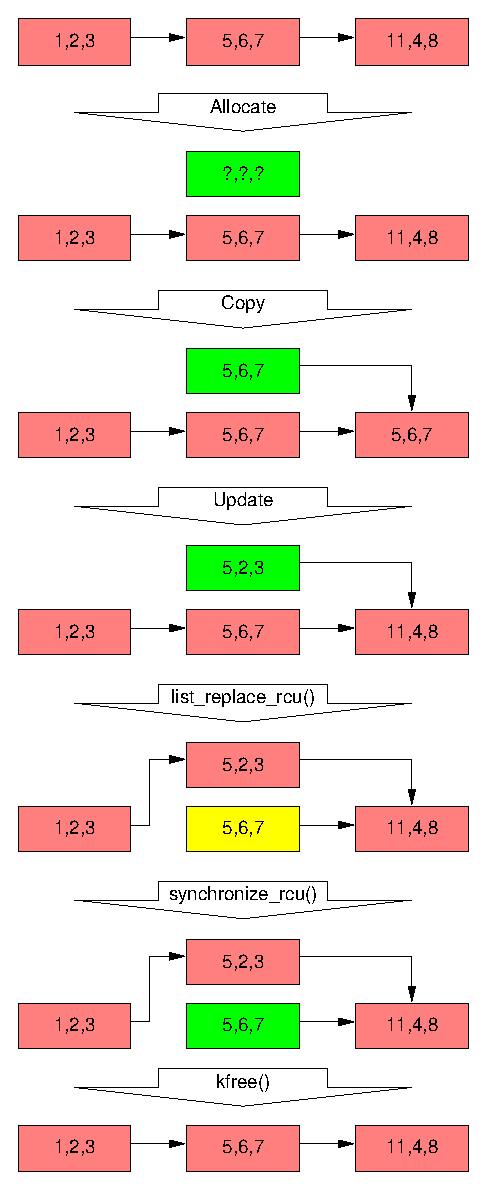
\includegraphics{defer/RCUReplacement}}
\caption{RCU Replacement in Linked List}
\label{fig:defer:RCU Replacement in Linked List}
\end{figure}

The initial state of the list, including the pointer \co{p},
is the same as for the deletion example, as shown on the
first row of
Figure~\ref{fig:defer:RCU Replacement in Linked List}.

As before,
the triples in each element represent the values of fields \co{a},
\co{b}, and \co{c}, respectively.
The red-shaded elements might be referenced by readers,
and because readers do not synchronize directly with updaters,
readers might run concurrently with this entire replacement process.
Please note that
we again omit the backwards pointers and the link from the tail
of the list to the head for clarity.

The following text describes how to replace the \co{5,6,7} element
with \co{5,2,3} in such a way that any given reader sees one of these
two values.

\begin{lineref}[ln:defer:Canonical RCU Replacement Example (2nd)]
Line~\lnref{kmalloc} \co{kmalloc()}s a replacement element, as follows,
resulting in the state as shown in the second row of
Figure~\ref{fig:defer:RCU Replacement in Linked List}.
At this point, no reader can hold a reference to the newly allocated
element (as indicated by its green shading), and it is uninitialized
(as indicated by the question marks).

Line~\lnref{copy} copies the old element to the new one, resulting in the
state as shown in the third row of
Figure~\ref{fig:defer:RCU Replacement in Linked List}.
The newly allocated element still cannot be referenced by readers, but
it is now initialized.

Line~\lnref{update1} updates \co{q->b} to the value ``2'', and
line~\lnref{update2} updates \co{q->c} to the value ``3'',
as shown on the fourth row of
Figure~\ref{fig:defer:RCU Replacement in Linked List}.

Now, line~\lnref{replace} does the replacement, so that the new element is
finally visible to readers, and hence is shaded red, as shown on
the fifth row of
Figure~\ref{fig:defer:RCU Replacement in Linked List}.
At this point, as shown below, we have two versions of the list.
Pre-existing readers might see the \co{5,6,7} element (which is
therefore now shaded yellow), but
new readers will instead see the \co{5,2,3} element.
But any given reader is guaranteed to see some well-defined list.

After the \co{synchronize_rcu()} on line~\lnref{sync_rcu} returns,
a grace period will have elapsed, and so all reads that started before the
\co{list_replace_rcu()} will have completed.
In particular, any readers that might have been holding references
to the \co{5,6,7} element are guaranteed to have exited
their RCU read-side critical sections, and are thus prohibited from
continuing to hold a reference.
Therefore, there can no longer be any readers holding references
to the old element, as indicated its green shading in the sixth row of
Figure~\ref{fig:defer:RCU Replacement in Linked List}.
As far as the readers are concerned, we are back to having a single version
of the list, but with the new element in place of the old.

After the \co{kfree()} on line~\lnref{kfree} completes, the list will
appear as shown on the final row of
Figure~\ref{fig:defer:RCU Replacement in Linked List}.
\end{lineref}

Despite the fact that RCU was named after the replacement case,
the vast majority of RCU usage within the Linux kernel relies on
the simple deletion case shown in
Section~\ref{sec:defer:Maintain Multiple Versions of Recently Updated Objects}.

\paragraph{Discussion}
\label{sec:defer:Discussion}

These examples assumed that a mutex was held across the entire
update operation, which would mean that there could be at most two
versions of the list active at a given time.

\QuickQuiz{}
	How would you modify the deletion example to permit more than two
	versions of the list to be active?
\QuickQuizAnswer{
	One way of accomplishing this is as shown in
	Listing~\ref{lst:defer:Concurrent RCU Deletion}.

\begin{listing}[htbp]
\begin{VerbatimL}
spin_lock(&mylock);
p = search(head, key);
if (p == NULL)
	spin_unlock(&mylock);
else {
	list_del_rcu(&p->list);
	spin_unlock(&mylock);
	synchronize_rcu();
	kfree(p);
}
\end{VerbatimL}
\caption{Concurrent RCU Deletion}
\label{lst:defer:Concurrent RCU Deletion}
\end{listing}

	Note that this means that multiple concurrent deletions might be
	waiting in \co{synchronize_rcu()}.
} \QuickQuizEnd

\QuickQuiz{}
	How many RCU versions of a given list can be
	active at any given time?
\QuickQuizAnswer{
	That depends on the synchronization design.
	If a semaphore protecting the update is held across the grace period,
	then there can be at most two versions, the old and the new.

	However, suppose that only the search, the update, and the
	\co{list_replace_rcu()} were protected by a lock, so that
	the \co{synchronize_rcu()} was outside of that lock, similar
	to the code shown in
	Listing~\ref{lst:defer:Concurrent RCU Deletion}.
	Suppose further that a large number of threads undertook an
	RCU replacement at about the same time, and that readers
	are also constantly traversing the data structure.

	Then the following sequence of events could occur, starting from
	the end state of
	Figure~\ref{fig:defer:RCU Replacement in Linked List}:

	\begin{enumerate}
	\item	Thread~A traverses the list, obtaining a reference to
		the 5,2,3 element.
	\item	Thread~B replaces the 5,2,3 element with a new
		5,2,4 element, then waits for its \co{synchronize_rcu()}
		call to return.
	\item	Thread~C traverses the list, obtaining a reference to
		the 5,2,4 element.
	\item	Thread~D replaces the 5,2,4 element with a new
		5,2,5 element, then waits for its \co{synchronize_rcu()}
		call to return.
	\item	Thread~E traverses the list, obtaining a reference to
		the 5,2,5 element.
	\item	Thread~F replaces the 5,2,5 element with a new
		5,2,6 element, then waits for its \co{synchronize_rcu()}
		call to return.
	\item	Thread~G traverses the list, obtaining a reference to
		the 5,2,6 element.
	\item	And the previous two steps repeat quickly, so that all
		of them happen before any of the \co{synchronize_rcu()}
		calls return.
	\end{enumerate}

	Thus, there can be an arbitrary number of versions active,
	limited only by memory and by how many updates could be completed
	within a grace period.
	But please note that data structures that are updated so frequently
	probably are not good candidates for RCU.
	That said, RCU can handle high update rates when necessary.
} \QuickQuizEnd

This sequence of events shows how RCU updates use multiple versions
to safely carry out changes in presence of concurrent readers.
Of course, some algorithms cannot gracefully handle multiple versions.
There are techniques
for adapting such algorithms to RCU~\cite{PaulEdwardMcKenneyPhD},
but these are beyond the scope of this section.

\subsubsection{Summary of RCU Fundamentals}
\label{sec:defer:Summary of RCU Fundamentals}

This section has described the three fundamental components of RCU-based
algorithms:

\begin{enumerate}
\item	a publish-subscribe mechanism for adding new data,

\item	a way of waiting for pre-existing RCU readers to finish,\footnote{
		This component is described in much greater detail in
		Section~\ref{sec:memorder:RCU}.}
	and

\item	a discipline of maintaining multiple versions to permit
	change without harming or unduly delaying concurrent RCU readers.
\end{enumerate}

\QuickQuiz{}
	How can RCU updaters possibly delay RCU readers, given that the
	\co{rcu_read_lock()} and \co{rcu_read_unlock()}
	primitives neither spin nor block?
\QuickQuizAnswer{
	The modifications undertaken by a given RCU updater will cause the
	corresponding CPU to invalidate cache lines containing the data,
	forcing the CPUs running concurrent RCU readers to incur expensive
	cache misses.
	(Can you design an algorithm that changes a data structure
	\emph{without}
	inflicting expensive cache misses on concurrent readers?
	On subsequent readers?)
} \QuickQuizEnd

These three RCU components
allow data to be updated in face of concurrent readers, and
can be combined in different ways to
implement a surprising variety of different types of RCU-based algorithms,
some of which are described in the following section.

% defer/rcuusage.tex
% mainfile: ../perfbook.tex
% SPDX-License-Identifier: CC-BY-SA-3.0

\subsection{RCU Usage}
\label{sec:defer:RCU Usage}
\OriginallyPublished{Section}{sec:defer:RCU Usage}{RCU Usage}{Linux Weekly News}{PaulEMcKenney2008WhatIsRCUUsage}

This section answers the question ``What is RCU?'' from the viewpoint
of the uses to which RCU can be put.
Because RCU is most frequently used to replace some existing mechanism,
we look at it primarily in terms of its relationship to such mechanisms,
as listed in \cref{tab:defer:RCU Usage}
and as displayed in \cref{fig:defer:Relationships Between RCU Use Cases}.
Following the sections listed in this table,
\cref{sec:defer:RCU Usage Summary} provides a summary.

\begin{table}
\renewcommand*{\arraystretch}{1.2}
\centering
\small
\begin{tabular}{ll}
\toprule
Mechanism RCU Replaces & Page \\
\midrule
RCU for pre-BSD routing &
	\pageref{sec:defer:RCU for Pre-BSD Routing} \\
Wait for pre-existing things to finish &
	\pageref{sec:defer:Wait for Pre-Existing Things to Finish} \\
Phased state change &
	\pageref{sec:defer:Phased State Change} \\
Add-only list (publish/subscribe) &
	\pageref{sec:defer:Add-Only List} \\
Type-safe memory &
	\pageref{sec:defer:Type-Safe Memory} \\
Light-weight garbage collector &
	\pageref{sec:defer:Light-Weight Garbage Collector} \\
Existence Guarantee &
	\pageref{sec:defer:Existence Guarantee} \\
Delete-only list &
	\pageref{sec:defer:Delete-Only List} \\
Quasi reader-writer lock &
	\pageref{sec:defer:Quasi Reader-Writer Lock} \\
Quasi reference count &
	\pageref{sec:defer:Quasi Reference Count} \\
Quasi multi-version concurrency control (MVCC) &
	\pageref{sec:defer:Quasi Multi-Version Concurrency Control} \\
\bottomrule
\end{tabular}
\caption{RCU Usage}
\label{tab:defer:RCU Usage}
\end{table}

\subsubsection{RCU for Pre-BSD Routing}
\label{sec:defer:RCU for Pre-BSD Routing}

In contrast to the later sections, this section focuses on a very
specific use case for the purpose of comparison with other mechanisms.

\Cref{lst:defer:RCU Pre-BSD Routing Table Lookup,%
lst:defer:RCU Pre-BSD Routing Table Add/Delete}
show code for an RCU-protected Pre-BSD routing table
(\path{route_rcu.c}).
The former shows data structures and \co{route_lookup()},
and the latter shows \co{route_add()} and \co{route_del()}.

\begin{listing}
\input{CodeSamples/defer/route_rcu@lookup.fcv}
\caption{RCU Pre-BSD Routing Table Lookup}
\label{lst:defer:RCU Pre-BSD Routing Table Lookup}
\end{listing}

\begin{listing}
\input{CodeSamples/defer/route_rcu@add_del.fcv}
\caption{RCU Pre-BSD Routing Table Add/Delete}
\label{lst:defer:RCU Pre-BSD Routing Table Add/Delete}
\end{listing}

\begin{fcvref}[ln:defer:route_rcu:lookup]
In \cref{lst:defer:RCU Pre-BSD Routing Table Lookup},
\clnref{rh} adds the \co{->rh} field used by RCU reclamation,
\clnref{re_freed} adds the \co{->re_freed} use-after-free-check field,
\clnref{lock,unlock1,unlock2}
add RCU read-side protection,
and \clnref{chk_freed,abort} add the use-after-free check.
\end{fcvref}
\begin{fcvref}[ln:defer:route_rcu:add_del]
In \cref{lst:defer:RCU Pre-BSD Routing Table Add/Delete},
\clnref{add:lock,add:unlock,del:lock,%
del:unlock1,del:unlock2} add update-side locking,
\clnref{add:add_rcu,del:del_rcu} add RCU update-side protection,
\clnref{del:call_rcu} causes \co{route_cb()} to be invoked after
a grace period elapses,
and \clnrefrange{cb:b}{cb:e} define \co{route_cb()}.
This is minimal added code for a working concurrent implementation.
\end{fcvref}

\begin{figure}
\centering
\resizebox{2.5in}{!}{\includegraphics{CodeSamples/defer/data/hps.2019.12.17a/perf-rcu}}
\caption{Pre-BSD Routing Table Protected by RCU}
\label{fig:defer:Pre-BSD Routing Table Protected by RCU}
\end{figure}

\Cref{fig:defer:Pre-BSD Routing Table Protected by RCU}
shows the performance on the read-only workload.
RCU scales quite well, and offers nearly ideal performance.
However, this data was generated using the \co{RCU_SIGNAL}
flavor of userspace
RCU~\cite{MathieuDesnoyers2009URCU,PaulMcKenney2013LWNURCU},
for which \co{rcu_read_lock()} and \co{rcu_read_unlock()}
generate a small amount of code.
What happens for the QSBR flavor of RCU, which generates no code at all
for \co{rcu_read_lock()} and \co{rcu_read_unlock()}?
(See \cref{sec:defer:Introduction to RCU},
and especially
\cref{fig:defer:QSBR: Waiting for Pre-Existing Readers},
for a discussion of RCU QSBR\@.)

The answer to this is shown in
\cref{fig:defer:Pre-BSD Routing Table Protected by RCU QSBR},
which shows that RCU QSBR's performance and scalability actually exceeds
that of the ideal synchronization-free workload.

\QuickQuizSeries{%
\QuickQuizB{
	Wait, what???
	How can RCU QSBR possibly be better than ideal?
	Just what rubbish definition of ideal would fail to be the best
	of all possible results???
}\QuickQuizAnswerB{
	This is an excellent question, and the answer is that modern
	CPUs and compilers are extremely complex.
	But before getting into that, it is well worth noting that
	RCU QSBR's performance advantage appears only in the
	one-hardware-thread-per-core regime.
	Once the system is fully loaded, RCU QSBR's performance drops
	back to ideal.

	The RCU variant of the \co{route_lookup()} search loop actually
	has one more x86 instruction than does the sequential version,
	namely the \co{lea} in the sequence
	\co{cmp}, \co{je}, \co{mov}, \co{cmp}, \co{lea}, and \co{jne}.
	This extra instruction is due to the \co{rcu_head} structure
	at the beginning of the RCU variant's \co{route_entry} structure,
	so that, unlike the sequential variant, the RCU variant's
	\co{->re_next.next} pointer has a non-zero offset.
	Back in the 1980s, this additional \co{lea} instruction might
	have reliably resulted in the RCU variant being slower, but we
	are now in the 21\textsuperscript{st} century, and the 1980s
	are long gone.

	But those of you who read
	\cref{sec:cpu:Pipelined CPUs}
	carefully already knew all of this!

	These counter-intuitive results of course means that any
	performance result on modern microprocessors must be subject to
	some skepticism.
	In theory, it really does not make sense to obtain performance
	results that are better than ideal, but it really can happen
	on modern microprocessors.
	Such results can be thought of as similar to the celebrated
	super-linear speedups (see
	\cref{sec:SMPdesign:Beyond Partitioning}
	for one such example), that is, of interest but also of limited
	practical importance.
	Nevertheless, one of the strengths of RCU is that its read-side
	overhead is so low that tiny effects such as this one are visible
	in real performance measurements.

\begin{figure}
\centering
% Run with initial rcu_head structure in route_entry moved down.
\resizebox{2.5in}{!}{\includegraphics{CodeSamples/defer/data/hps.2019.12.17a/perf-rcu-qsbr}}
\caption{Pre-BSD Routing Table Protected by RCU QSBR With Non-Initial \tco{rcu_head}}
\label{fig:defer:Pre-BSD Routing Table Protected by RCU QSBR With Non-Initial rcu-head}
\end{figure}

	This raises the question as to what would happen if the
	\co{rcu_head} structure were to be moved so that RCU's
	\co{->re_next.next} pointer also had zero offset, just the
	same as the sequential variant.
	And the answer, as can be seen in
	\cref{fig:defer:Pre-BSD Routing Table Protected by RCU QSBR With Non-Initial rcu-head},
	is that this causes RCU QSBR's performance to decrease to where
	it is still very nearly ideal, but no longer super-ideal.
}\QuickQuizEndB
%
\QuickQuizE{
	Given RCU QSBR's read-side performance, why bother with any
	other flavor of userspace RCU?
}\QuickQuizAnswerE{
	Because RCU QSBR places constraints on the overall application
	that might not be tolerable,
	for example, requiring that each and every thread in the
	application regularly pass through a quiescent state.
	Among other things, this means that RCU QSBR is not helpful
	to library writers, who might be better served by other
	flavors of userspace RCU~\cite{PaulMcKenney2013LWNURCU}.
}\QuickQuizEndE
}

\begin{figure}
\centering
% Run with initial rcu_head structure at beginning of route_entry structure.
% This need to run twice is the reason for the oddball directory.
% @@@ Make this generate both files with a single run?
\resizebox{2.5in}{!}{\includegraphics{CodeSamples/defer/data/hps.2019.12.02a/perf-rcu-qsbr}}
\caption{Pre-BSD Routing Table Protected by RCU QSBR}
\label{fig:defer:Pre-BSD Routing Table Protected by RCU QSBR}
\end{figure}

\begin{figure*}
\centering
\IfTwoColumn{
  \resizebox{5.5in}{!}{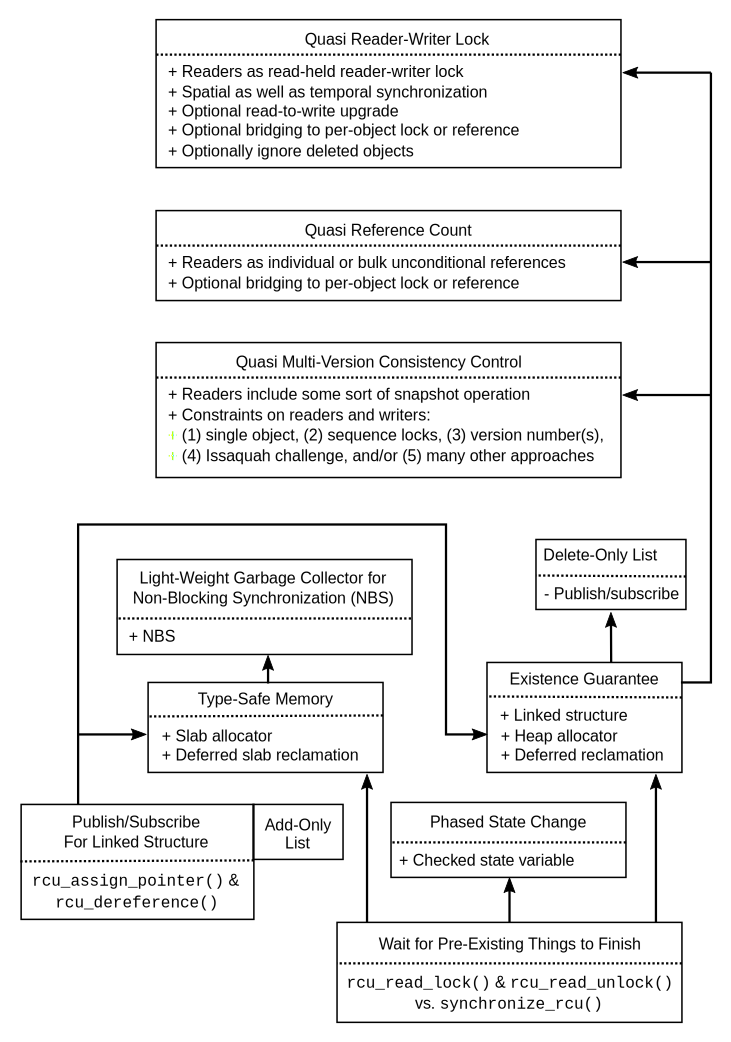
\includegraphics{defer/RCUusecases}}
}{
  \resizebox{.96\textwidth}{!}{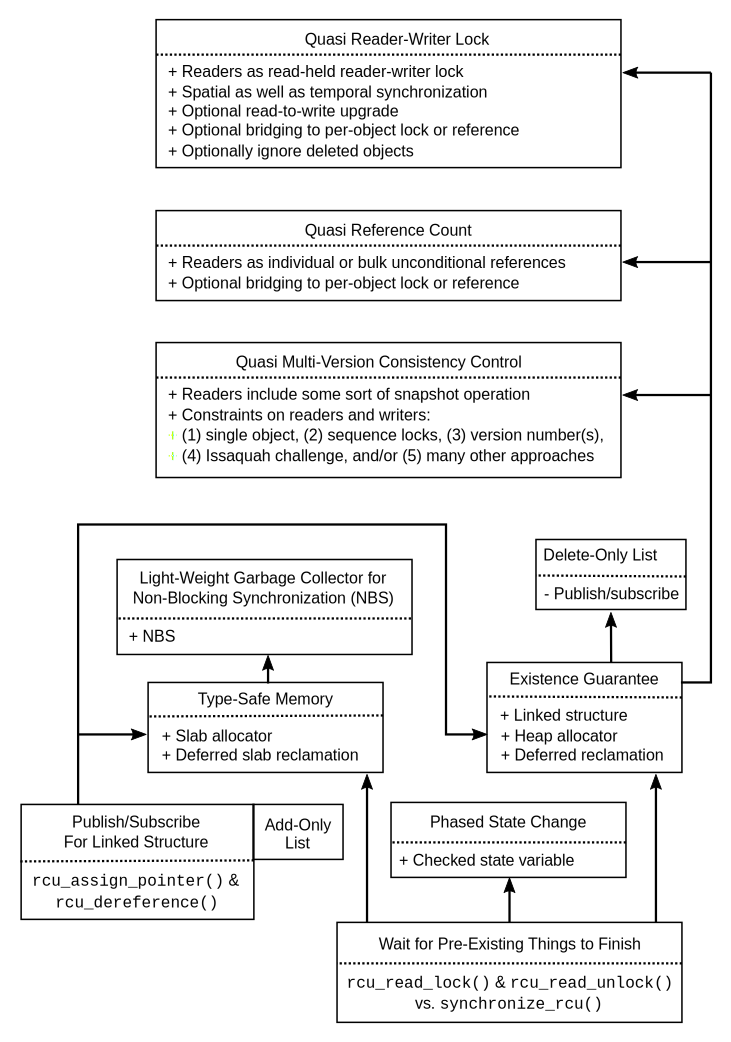
\includegraphics{defer/RCUusecases}}
  % eb builds require .96
}
\caption{Relationships Between RCU Use Cases}
\label{fig:defer:Relationships Between RCU Use Cases}
\end{figure*}

Although Pre-BSD routing is an excellent RCU use case, it is worthwhile
looking at the relationships betweeen the wider spectrum of use cases
shown in
\cref{fig:defer:Relationships Between RCU Use Cases}.
This task is taken up by the following sections.

While reading these sections, please ask yourself which of these
use cases best describes Pre-BSD routing.

\subsubsection{Wait for Pre-Existing Things to Finish}
\label{sec:defer:Wait for Pre-Existing Things to Finish}

As noted in \cref{sec:defer:RCU Fundamentals}
an important component
of RCU is a way of waiting for RCU readers to finish.
One of
RCU's great strength is that it allows you to wait for each of
thousands of different things to finish without having to explicitly
track each and every one of them, and without incurring
the performance degradation, scalability limitations, complex deadlock
scenarios, and memory-leak hazards that are inherent in schemes that
use explicit tracking.

In this section, we will show how \co{synchronize_sched()}'s
read-side counterparts (which include anything that disables preemption,
along with hardware operations and
primitives that disable interrupts) permit you to interaction with
non-maskable interrupt
(NMI) handlers, which is quite difficult using locking.
This approach has been called ``Pure RCU''~\cite{PaulEdwardMcKenneyPhD},
and it is used in a few places in the Linux kernel.

The basic form of such ``Pure RCU'' designs is as follows:

\begin{enumerate}
\item	Make a change, for example, to the way that the OS reacts to an NMI\@.
\item	Wait for all pre-existing read-side critical sections to
	completely finish (for example, by using the
	\co{synchronize_sched()} primitive).\footnote{
		In Linux kernel v5.1 and later, \co{synchronize_sched()} has
		been subsumed into \co{synchronize_rcu()}.}
	The key observation here is that subsequent RCU read-side critical
	sections are guaranteed to see whatever change was made.
\item	Clean up, for example, return status indicating that the
	change was successfully made.
\end{enumerate}

The remainder of this section presents example code adapted from
the Linux kernel.
In this example, the \co{timer_stop()} function in the now-defunct
oprofile facility uses \co{synchronize_sched()} to ensure that all
in-flight NMI notifications have completed before freeing the associated
resources.
A simplified version of this code is shown in
\cref{lst:defer:Using RCU to Wait for NMIs to Finish}.

\begin{listing}
\begin{fcvlabel}[ln:defer:Using RCU to Wait for NMIs to Finish]
\begin{VerbatimL}[commandchars=\\\@\$]
struct profile_buffer {				\lnlbl@struct:b$
	long size;
	atomic_t entry[0];
};						\lnlbl@struct:e$
static struct profile_buffer *buf = NULL;	\lnlbl@struct:buf$

void nmi_profile(unsigned long pcvalue)		\lnlbl@nmi_profile:b$
{
	struct profile_buffer *p = rcu_dereference(buf);\lnlbl@nmi_profile:rcu_deref$

	if (p == NULL)				\lnlbl@nmi_profile:if_NULL$
		return;				\lnlbl@nmi_profile:ret:a$
	if (pcvalue >= p->size)			\lnlbl@nmi_profile:if_oor$
		return;				\lnlbl@nmi_profile:ret:b$
	atomic_inc(&p->entry[pcvalue]);		\lnlbl@nmi_profile:inc$
}						\lnlbl@nmi_profile:e$

void nmi_stop(void)				\lnlbl@nmi_stop:b$
{
	struct profile_buffer *p = buf;		\lnlbl@nmi_stop:fetch$

	if (p == NULL)				\lnlbl@nmi_stop:if_NULL$
		return;				\lnlbl@nmi_stop:ret$
	rcu_assign_pointer(buf, NULL);		\lnlbl@nmi_stop:NULL$
	synchronize_sched();			\lnlbl@nmi_stop:sync_sched$
	kfree(p);				\lnlbl@nmi_stop:kfree$
}						\lnlbl@nmi_stop:e$
\end{VerbatimL}
\end{fcvlabel}
\caption{Using RCU to Wait for NMIs to Finish}
\label{lst:defer:Using RCU to Wait for NMIs to Finish}
\end{listing}

\begin{fcvref}[ln:defer:Using RCU to Wait for NMIs to Finish:struct]
\Clnrefrange{b}{e} define a \co{profile_buffer} structure, containing a
size and an indefinite array of entries.
\Clnref{buf} defines a pointer to a profile buffer, which is
presumably initialized elsewhere to point to a dynamically allocated
region of memory.
\end{fcvref}

\begin{fcvref}[ln:defer:Using RCU to Wait for NMIs to Finish:nmi_profile]
\Clnrefrange{b}{e} define the \co{nmi_profile()} function,
which is called from within an NMI handler.
As such, it cannot be preempted, nor can it be interrupted by a normal
interrupt handler, however, it is still subject to delays due to cache misses,
ECC errors, and cycle stealing by other hardware threads within the same
core.
\Clnref{rcu_deref} gets a local pointer to the profile buffer using the
\co{rcu_dereference()} primitive to ensure memory ordering on
DEC Alpha, and
\clnref{if_NULL,ret:a} exit from this function if there is no
profile buffer currently allocated, while \clnref{if_oor,ret:b}
exit from this function if the \co{pcvalue} argument
is out of range.
Otherwise, \clnref{inc} increments the profile-buffer entry indexed
by the \co{pcvalue} argument.
Note that storing the size with the buffer guarantees that the
range check matches the buffer, even if a large buffer is suddenly
replaced by a smaller one.
\end{fcvref}

\begin{fcvref}[ln:defer:Using RCU to Wait for NMIs to Finish:nmi_stop]
\Clnrefrange{b}{e} define the \co{nmi_stop()} function,
where the caller is responsible for mutual exclusion (for example,
holding the correct lock).
\Clnref{fetch} fetches a pointer to the profile buffer, and
\clnref{if_NULL,ret} exit the function if there is no buffer.
Otherwise, \clnref{NULL} \co{NULL}s out the profile-buffer pointer
(using the \co{rcu_assign_pointer()} primitive to maintain
memory ordering on weakly ordered machines),
and \clnref{sync_sched} waits for an RCU Sched grace period to elapse,
in particular, waiting for all non-preemptible regions of code,
including NMI handlers, to complete.
Once execution continues at \clnref{kfree}, we are guaranteed that
any instance of \co{nmi_profile()} that obtained a
pointer to the old buffer has returned.
It is therefore safe to free the buffer, in this case using the
\co{kfree()} primitive.
\end{fcvref}

\QuickQuiz{
	Suppose that the \co{nmi_profile()} function was preemptible.
	What would need to change to make this example work correctly?
}\QuickQuizAnswer{
	One approach would be to use
	\co{rcu_read_lock()} and \co{rcu_read_unlock()}
	in \co{nmi_profile()}, and to replace the
	\co{synchronize_sched()} with \co{synchronize_rcu()},
	perhaps as shown in
	\cref{lst:defer:Using RCU to Wait for Mythical Preemptible NMIs to Finish}.
%
\begin{listing}
\begin{VerbatimL}
struct profile_buffer {
	long size;
	atomic_t entry[0];
};
static struct profile_buffer *buf = NULL;

void nmi_profile(unsigned long pcvalue)
{
	struct profile_buffer *p;

	rcu_read_lock();
	p = rcu_dereference(buf);
	if (p == NULL) {
		rcu_read_unlock();
		return;
	}
	if (pcvalue >= p->size) {
		rcu_read_unlock();
		return;
	}
	atomic_inc(&p->entry[pcvalue]);
	rcu_read_unlock();
}

void nmi_stop(void)
{
	struct profile_buffer *p = buf;

	if (p == NULL)
		return;
	rcu_assign_pointer(buf, NULL);
	synchronize_rcu();
	kfree(p);
}
\end{VerbatimL}
\caption{Using RCU to Wait for Mythical Preemptible NMIs to Finish}
\label{lst:defer:Using RCU to Wait for Mythical Preemptible NMIs to Finish}
\end{listing}
%
}\QuickQuizEnd

In short, RCU makes it easy to dynamically switch among profile
buffers (you just \emph{try} doing this efficiently with atomic
operations, or at all with locking!).
This is a rare use of RCU in its pure form.
RCU is normally used at higher levels of abstraction, as
will be shown in the following sections.

\subsubsection{Phased State Change}
\label{sec:defer:Phased State Change}

\Cref{fig:defer:Phased State Change for Maintenance Operation}
shows a timeline for an example phased state change to efficiently
handle maintenance operations.
If there is no maintenance operation in progress, common-case operations
must proceed quickly, for example, without acquiring a reader-writer lock.
However, if there is a maintenance operation in progress, the common-case
operations must be undertaken carefully, taking into account added
complexities due to their running concurrently with that maintenance
operation.
This means that common-case operations will incur higher overhead during
maintenance operations, which is one reason that maintenance operations
are normally scheduled to take place during times of low load.

\begin{figure}
\centering
\resizebox{\twocolumnwidth}{!}{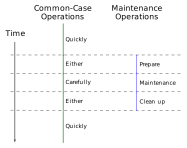
\includegraphics{defer/RCUphasedstatechange}}
\caption{Phased State Change for Maintenance Operation}
\label{fig:defer:Phased State Change for Maintenance Operation}
\end{figure}

In the figure, these apparently conflicting requirements are resolved by
having a prepare phase prior to the maintenance operation and a cleanup
phase after it, during which the common-case operations can proceed
either quickly or carefully.

\begin{listing}
\begin{fcvlabel}[ln:defer:Phased State Change for Maintenance Operations]
\begin{VerbatimL}[commandchars=\\\@\$]
bool be_careful;

void cco(void)
{
	rcu_read_lock();			\lnlbl@rrl$
	if (READ_ONCE(be_careful))		\lnlbl@if$
		cco_carefully();		\lnlbl@careful$
	else
		cco_quickly();			\lnlbl@quick$
	rcu_read_unlock();			\lnlbl@rul$
}

void maint(void)
{
	WRITE_ONCE(be_careful, true);		\lnlbl@tocareful$
	synchronize_rcu();			\lnlbl@sr1$
	do_maint();				\lnlbl@maint$
	synchronize_rcu();			\lnlbl@sr2$
	WRITE_ONCE(be_careful, false);		\lnlbl@toquick$
}
\end{VerbatimL}
\end{fcvlabel}
\caption{Phased State Change for Maintenance Operations}
\label{lst:defer:Phased State Change for Maintenance Operations}
\end{listing}

\begin{fcvref}[ln:defer:Phased State Change for Maintenance Operations]
Example pseudo-code for this phased state change is shown in
\cref{lst:defer:Phased State Change for Maintenance Operations}.
The common-case operations are carried out by \co{cco()} within an RCU
read-side critical section extending from \clnref{rrl} to \clnref{rul}.
Here, \clnref{if} checks a global \co{be_careful} flag, invoking
\co{cco_carefully()} or \co{cco_quickly()}, as indicated.
\end{fcvref}

\begin{fcvref}[ln:defer:Phased State Change for Maintenance Operations]
This allows the \co{maint()} function to set the \co{be_careful} flag
on \clnref{tocareful} and wait for an RCU grace period on \clnref{sr1}.
When control reaches \clnref{maint}, all \co{cco()} functions that saw a
\co{false} value of \co{be_careful} (and thus which might invoke
the \co{cco_quickly()} function) will have completed their operations,
so that all currently executing \co{cco()} functions will be invoking
\co{cco_carefully()}.
This means that it is safe for the \co{do_maint()} function to be
invoked.
\Clnref{sr2} then waits for all \co{cco()} functions that might have
run concurrently with \co{do_maint()} to complete, and finally
\clnref{toquick} sets the \co{be_careful} flag back to \co{false}.
\end{fcvref}

\QuickQuiz{
	What is the point of the second call to \co{synchronize_rcu()}
	in function
	\co{maint()} in \cref{lst:defer:Phased State Change for Maintenance Operations}?
	Isn't it OK for any \co{cco()} invocations in the clean-up
	phase to invoke either \co{cco_carefully()} or \co{cco_quickly()}?
}\QuickQuizAnswer{
	The problem is that there is no ordering between the \co{cco()}
	function's load from \co{be_careful} and any memory loads
	executed by the \co{cco_quickly()} function.
	Because there is no ordering, without that second call to
	\co{syncrhonize_rcu()}, memory ordering could cause loads
	in \co{cco_quickly()} to overlap with stores by \co{do_maint()}.

	Another alternative would be to compensate for the removal of
	that second call to \co{synchronize_rcu()} by changing the
	\co{READ_ONCE()} to \co{smp_load_acquire()} and the
	\co{WRITE_ONCE()} to \co{smp_store_release()}, thus restoring
	the needed ordering.
}\QuickQuizEnd

\QuickQuiz{
	How can you be sure that the code shown in
	\co{maint()} in \cref{lst:defer:Phased State Change for Maintenance Operations}
	really works?\@
}\QuickQuizAnswer{
	By one popular school of thought, you cannot.

	But in this case, those willing to jump ahead to
	\cref{chp:Formal Verification}
	and
	\cref{chp:Advanced Synchronization: Memory Ordering}
	might find a couple of LKMM litmus tests to be interesting
	(\path{C-RCU-phased-state-change-1.litmus} and
	\path{C-RCU-phased-state-change-2.litmus}).
	These tests could be argued to demonstrate that this code
	and a variant of it really do work.
}\QuickQuizEnd

Phased state change allows frequent operations to use light-weight
checks, without the need for expensive lock acquisitions or atomic
read-modify-write operations.
Phased state change adds only a checked state variable
to the wait-to-finish use case
(\cref{sec:defer:Wait for Pre-Existing Things to Finish}),
thus also residing at a rather low level of abstraction.

\subsubsection{Add-Only List}
\label{sec:defer:Add-Only List}

Add-only data structures, exemplified by the add-only list, can be used
for a surprisingly common set of use cases, perhaps most commonly the
logging of changes.
Add-only data structures are a pure use of RCU's underlying
publish/subscribe mechanism.

An add-only variant of a pre-BSD routing table can be derived from
\cref{lst:defer:RCU Pre-BSD Routing Table Lookup,lst:defer:RCU Pre-BSD Routing Table Add/Delete}.
Because there is no deletion, the \co{route_del()} and \co{route_cb()}
functions may be dispensed with, along with the \co{->rh}
and \co{->re_freed} fields of the \co{route_entry} structure, the
\co{rcu_read_lock()}, the \co{rcu_read_unlock()} invocations in the
\co{route_lookup()} function, and all uses of the \co{->re_freed} field
in all remaining functions.

Of course, if there are many concurrent invocations of the \co{route_add()}
function, there will be heavy contention on \co{routelock}, and if lockless
techniques are used, heavy memory contention on \co{routelist}.
The usual way to avoid this contention is to use a concurrency-friendly
data structure such as a hash table (see \cref{chp:Data Structures}).
Alternatively, per-CPU data structures might be periodically merged
into a single global data structure.

On the other hand, if there is never any deletion, extended time periods
featuring many concurrent invocations of \co{route_add()} will eventually
consume all available memory.
Therefore, most RCU-protected data structures also implement deletion.

\subsubsection{Type-Safe Memory}
\label{sec:defer:Type-Safe Memory}

A number of lockless algorithms do not require that a given data
element keep the same identity through a given RCU read-side critical
section referencing it---but only if that data element retains the
same type.
In other words, these lockless algorithms can tolerate a given data
element being freed and reallocated as the same type of structure
while they are referencing it, but must prohibit a change in type.
This guarantee, called ``type-safe memory'' in
academic literature~\cite{Cheriton96a},
is weaker than the existence guarantees discussed
in \cref{sec:defer:Existence Guarantee},
and is therefore quite a bit harder to work with.
Type-safe memory algorithms in the Linux kernel make use of slab caches,
specially marking these caches with \co{SLAB_TYPESAFE_BY_RCU}
so that RCU is used when returning a freed-up
slab to system memory.
This use of RCU guarantees that any in-use element of
such a slab will remain in that slab, thus retaining its type,
for the duration of any pre-existing RCU read-side critical sections.

\QuickQuiz{
	But what if there is an arbitrarily long series of RCU
	read-side critical sections in multiple threads, so that at
	any point in time there is at least one thread in the system
	executing in an RCU read-side critical section?
	Wouldn't that prevent any data from a \co{SLAB_TYPESAFE_BY_RCU}
	slab ever being returned to the system, possibly resulting
	in OOM events?
}\QuickQuizAnswer{
	There could certainly be an arbitrarily long period of time
	during which at least one thread is always in an RCU read-side
	critical section.
	However, the key words in the description in
	\cref{sec:defer:Type-Safe Memory}
	are ``in-use'' and ``pre-existing''.
	Keep in mind that a given RCU read-side critical section is
	conceptually only permitted to gain references to data elements
	that were in use at the beginning of that critical section.
	Furthermore, remember that a slab cannot be returned to the
	system until all of its data elements have been freed, in fact,
	the RCU grace period cannot start until after they have all been
	freed.

	Therefore, the slab cache need only wait for those RCU read-side
	critical sections that started before the freeing of the last element
	of the slab.
	This in turn means that any RCU grace period that begins after
	the freeing of the last element will do---the slab may be returned
	to the system after that grace period ends.
}\QuickQuizEnd

It is important to note that \co{SLAB_TYPESAFE_BY_RCU} will
\emph{in no way}
prevent \co{kmem_cache_alloc()} from immediately reallocating
memory that was just now freed via \co{kmem_cache_free()}!
In fact, the \co{SLAB_TYPESAFE_BY_RCU}-protected data structure
just returned by \co{rcu_dereference} might be freed and reallocated
an arbitrarily large number of times, even when under the protection
of \co{rcu_read_lock()}.
Instead, \co{SLAB_TYPESAFE_BY_RCU} operates by preventing
\co{kmem_cache_free()}
from returning a completely freed-up slab of data structures
to the system until after an RCU grace period elapses.
In short, although a given RCU read-side critical section might see a
given \co{SLAB_TYPESAFE_BY_RCU} data element being freed and reallocated
arbitrarily often, the element's type is guaranteed not to change until
that critical section has completed.

These algorithms therefore typically use a validation step that checks
to make sure that the newly referenced data structure really is the one
that was requested~\cite[Section~2.5]{LaninShasha1986TSM}.
These validation checks require that portions of the data structure
remain untouched by the free-reallocate process.
Such validation checks are usually very hard to get right, and can
hide subtle and difficult bugs.

Therefore, although type-safety-based lockless algorithms can be extremely
helpful in a very few difficult situations, you should instead use existence
guarantees where possible.
Simpler is after all almost always better!
On the other hand, type-safety-based lockless algorithms can
provide improved cache locality, and thus improved performance.
This improved cache locality is provided by the fact that such
algorithms can immediately reallocate a newly freed block of memory.
In contrast, algorithms based on existence guarantees must wait for
all pre-existing readers before reallocating memory, by which time
that memory may have been ejected from CPU caches.

As can be seen in \cref{fig:defer:Relationships Between RCU Use Cases},
RCU's type-safe-memory use case combines both the wait-to-finish
and publish-subscribe components, but in the Linux kernel also includes
the slab allocator's deferred reclamation specified by the
\co{SLAB_TYPESAFE_BY_RCU} flag.

\subsubsection{Light-Weight Garbage Collector}
\label{sec:defer:Light-Weight Garbage Collector}

A not-uncommon exclamation made by people first learning about
RCU is ``RCU is sort of like a garbage collector!''
This exclamation has a large grain of truth, but it can also be
misleading.

Perhaps the best way to think of the relationship between RCU
and automatic garbage collectors (GCs) is that RCU resembles
a GC in that the \emph{timing} of collection is automatically
determined, but that RCU differs from a GC in that:
\begin{enumerate*}[(1)]
\item The programmer must manually indicate when a given data
structure is eligible to be collected and
\item The programmer must manually mark the RCU read-side critical
sections where references might be held.
\end{enumerate*}

Despite these differences, the resemblance does go quite deep.
In fact, the first RCU-like mechanism I am aware of used a
reference-count-based garbage collector to handle the grace
periods~\cite{Kung80}, and the connection between RCU and
garbage collection has been noted more
recently~\cite{HarshalSheth2016goRCU}.

The light-weight garbage collector use case is very similar to
the type-safe-memory use case, adding only the desired non-blocking
algorithm to the mix.
This light-weight garbage collector use case can also be used in
conjunction with the existence guarantees described in the next section.

\subsubsection{Existence Guarantee}
\label{sec:defer:Existence Guarantee}

Gamsa et al.~\cite{Gamsa99}
discuss existence guarantees and describe how a mechanism
resembling RCU can be used to provide these existence guarantees
(see Section~5 on page 7 of the PDF), and
\cref{sec:locking:Lock-Based Existence Guarantees}
discusses how to guarantee existence via locking, along with the
ensuing disadvantages of doing so.
The effect is that if any RCU-protected data element is accessed
within an RCU read-side critical section, that data element is
guaranteed to remain in existence for the duration of that RCU
read-side critical section.

\begin{listing}
\begin{fcvlabel}[ln:defer:Existence Guarantees Enable Per-Element Locking]
\begin{VerbatimL}[commandchars=\\\@\$]
int delete(int key)
{
	struct element *p;
	int b;

	b = hashfunction(key);			\lnlbl@hash$
	rcu_read_lock();			\lnlbl@rdlock$
	p = rcu_dereference(hashtable[b]);
	if (p == NULL || p->key != key) {	\lnlbl@chkkey$
		rcu_read_unlock();		\lnlbl@rdunlock1$
		return 0;			\lnlbl@ret_0:a$
	}
	spin_lock(&p->lock);			\lnlbl@acq$
	if (hashtable[b] == p && p->key == key) {\lnlbl@chkkey2$
		rcu_read_unlock();		\lnlbl@rdunlock2$
		rcu_assign_pointer(hashtable[b], NULL);\lnlbl@remove$
		spin_unlock(&p->lock);		\lnlbl@rel1$
		synchronize_rcu();		\lnlbl@sync_rcu$
		kfree(p);			\lnlbl@kfree$
		return 1;			\lnlbl@ret_1$
	}
	spin_unlock(&p->lock);			\lnlbl@rel2$
	rcu_read_unlock();			\lnlbl@rdunlock3$
	return 0;				\lnlbl@ret_0:b$
}
\end{VerbatimL}
\end{fcvlabel}
\caption{Existence Guarantees Enable Per-Element Locking}
\label{lst:defer:Existence Guarantees Enable Per-Element Locking}
\end{listing}

\begin{fcvref}[ln:defer:Existence Guarantees Enable Per-Element Locking]
\Cref{lst:defer:Existence Guarantees Enable Per-Element Locking}
demonstrates how RCU-based existence guarantees can enable
per-element locking via a function that deletes an element from
a hash table.
\Clnref{hash} computes a hash function, and \clnref{rdlock} enters an RCU
read-side critical section.
If \clnref{chkkey} finds that the corresponding bucket of the hash table is
empty or that the element present is not the one we wish to delete,
then \clnref{rdunlock1} exits the RCU read-side critical section and
\clnref{ret_0:a}
indicates failure.
\end{fcvref}

\QuickQuiz{
	What if the element we need to delete is not the first element
	of the list on
	\clnrefr{ln:defer:Existence Guarantees Enable Per-Element Locking:chkkey} of
	\cref{lst:defer:Existence Guarantees Enable Per-Element Locking}?
}\QuickQuizAnswer{
	As with
	\cref{lst:locking:Per-Element Locking Without Existence Guarantees},
	this is a very simple hash table with no chaining, so the only
	element in a given bucket is the first element.
	The reader is again invited to adapt this example to a hash table with
	full chaining.
	Less energetic reader might wish to refer to
	\cref{chp:Data Structures}.
}\QuickQuizEnd

\begin{fcvref}[ln:defer:Existence Guarantees Enable Per-Element Locking]
Otherwise, \clnref{acq} acquires the update-side spinlock, and
\clnref{chkkey2} then checks that the element is still the one that we want.
If so, \clnref{rdunlock2} leaves the RCU read-side critical section,
\clnref{remove} removes it from the table, \clnref{rel1} releases
the lock, \clnref{sync_rcu} waits for all pre-existing RCU read-side critical
sections to complete, \clnref{kfree} frees the newly removed element,
and \clnref{ret_1} indicates success.
If the element is no longer the one we want, \clnref{rel2} releases
the lock, \clnref{rdunlock3} leaves the RCU read-side critical section,
and \clnref{ret_0:b} indicates failure to delete the specified key.
\end{fcvref}

\QuickQuizSeries{%
\QuickQuizB{
	\begin{fcvref}[ln:defer:Existence Guarantees Enable Per-Element Locking]
	Why is it OK to exit the RCU read-side critical section on
	\clnref{rdunlock2} of
	\cref{lst:defer:Existence Guarantees Enable Per-Element Locking}
	before releasing the lock on \clnref{rel1}?
	\end{fcvref}
}\QuickQuizAnswerB{
	\begin{fcvref}[ln:defer:Existence Guarantees Enable Per-Element Locking]
	First, please note that the second check on \clnref{chkkey2} is
	necessary because some other
	CPU might have removed this element while we were waiting
	to acquire the lock.
	However, the fact that we were in an RCU read-side critical section
	while acquiring the lock guarantees that this element could not
	possibly have been re-allocated and re-inserted into this
	hash table.
	Furthermore, once we acquire the lock, the lock itself guarantees
	the element's existence, so we no longer need to be in an
	RCU read-side critical section.

	The question as to whether it is necessary to re-check the
	element's key is left as an exercise to the reader.
	% A re-check is necessary if the key can mutate or if it is
	% necessary to reject deleted entries (in cases where deletion
	% is recorded by mutating the key.
	\end{fcvref}
}\QuickQuizEndB
%
\QuickQuizE{
	\begin{fcvref}[ln:defer:Existence Guarantees Enable Per-Element Locking]
	Why not exit the RCU read-side critical section on
	\clnref{rdunlock3} of
	\cref{lst:defer:Existence Guarantees Enable Per-Element Locking}
	before releasing the lock on \clnref{rel2}?
	\end{fcvref}
}\QuickQuizAnswerE{
	Suppose we reverse the order of these two lines.
	Then this code is vulnerable to the following sequence of
	events:
	\begin{enumerate}
	\begin{fcvref}[ln:defer:Existence Guarantees Enable Per-Element Locking]
	\item	CPU~0 invokes \co{delete()}, and finds the element
		to be deleted, executing through \clnref{rdunlock2}.
		It has not yet actually deleted the element, but
		is about to do so.
	\item	CPU~1 concurrently invokes \co{delete()}, attempting
		to delete this same element.
		However, CPU~0 still holds the lock, so CPU~1 waits
		for it at \clnref{acq}.
	\item	CPU~0 executes \clnref{remove,rel1},
		and blocks at \clnref{sync_rcu} waiting for CPU~1
		to exit its RCU read-side critical section.
	\item	CPU~1 now acquires the lock, but the test on \clnref{chkkey2}
		fails because CPU~0 has already removed the element.
		CPU~1 now executes \clnref{rel2}
		(which we switched with \clnref{rdunlock3}
		for the purposes of this Quick Quiz)
		and exits its RCU read-side critical section.
	\item	CPU~0 can now return from \co{synchronize_rcu()},
		and thus executes \clnref{kfree}, sending the element to
		the freelist.
	\item	CPU~1 now attempts to release a lock for an element
		that has been freed, and, worse yet, possibly
		reallocated as some other type of data structure.
		This is a fatal memory-corruption error.
	\end{fcvref}
	\end{enumerate}
}\QuickQuizEndE
}

Alert readers will recognize this as only a slight variation on
the original wait-to-finish theme
(\cref{sec:defer:Wait for Pre-Existing Things to Finish}),
adding publish/subscribe, linked structures, a heap allocator
(typically), and deferred reclamation, as shown in
\cref{fig:defer:Relationships Between RCU Use Cases}.
They might also note the deadlock-immunity advantages over the lock-based
existence guarantees discussed in
\cref{sec:locking:Lock-Based Existence Guarantees}.

\subsubsection{Delete-Only List}
\label{sec:defer:Delete-Only List}

The delete-only list is the less-popular counterpart to the add-only list
covered in \cref{sec:defer:Add-Only List}, and can be thought of as the
existence-guarantee use case, but without the publish/subscribe component,
as shown in \cref{fig:defer:Relationships Between RCU Use Cases}.
A delete-only list can be used when the universe of possible members of
the list is known at initialization, and where members can be removed.
For example, elements of the list might represent hardware elements of
the system that are subject to failure, but cannot be repaired or
replaced without a reboot.

An delete-only variant of a pre-BSD routing table can be derived from
\cref{lst:defer:RCU Pre-BSD Routing Table Lookup,lst:defer:RCU Pre-BSD Routing Table Add/Delete}.
Because there is no addition, the \co{route_add()} function may be
dispensed with, or, alternatively, its use might be restricted to
initialization time.
In theory, the \co{route_lookup()} function can use a non-RCU iterator,
though in the Linux kernel this will result in complaints from debug code.
In addition, the incremental cost of an RCU iterator is usually
negligible.

As a result, delete-only situations typically use algorithms and data
structures that are designed for addition as well as deletion.

\subsubsection{Quasi Reader-Writer Lock}
\label{sec:defer:Quasi Reader-Writer Lock}

Perhaps the most common use of RCU within the Linux kernel is as
a replacement for reader-writer locking in read-intensive situations.
Nevertheless, this use of RCU was not immediately apparent to me
at the outset.
In fact, I chose to implement a lightweight reader-writer
lock~\cite{WilsonCHsieh92a}\footnote{
	Similar to \co{brlock} in the 2.4 Linux kernel and to
	\co{lglock} in more recent Linux kernels.}
before implementing a general-purpose RCU implementation
back in the early 1990s.
Each and every one of the uses I envisioned for the lightweight reader-writer
lock was instead implemented using RCU\@.
In fact, it was more than
three years before the lightweight reader-writer lock saw its first use.
Boy, did I feel foolish!

The key similarity between RCU and reader-writer locking is that
both have read-side critical sections that can execute concurrently.
In fact, in some cases, it is possible to mechanically substitute RCU API
members for the corresponding reader-writer lock API members.
But first, why bother?

Advantages of RCU include performance,
deadlock immunity, and realtime latency.
There are, of course, limitations to RCU, including the fact that
readers and updaters run concurrently, that low-priority RCU readers
can block high-priority threads waiting for a grace period to elapse,
and that grace-period latencies can extend for many milliseconds.
These advantages and limitations are discussed in the following sections.

\paragraph{Performance}

\begin{figure}
\centering
\resizebox{2.5in}{!}{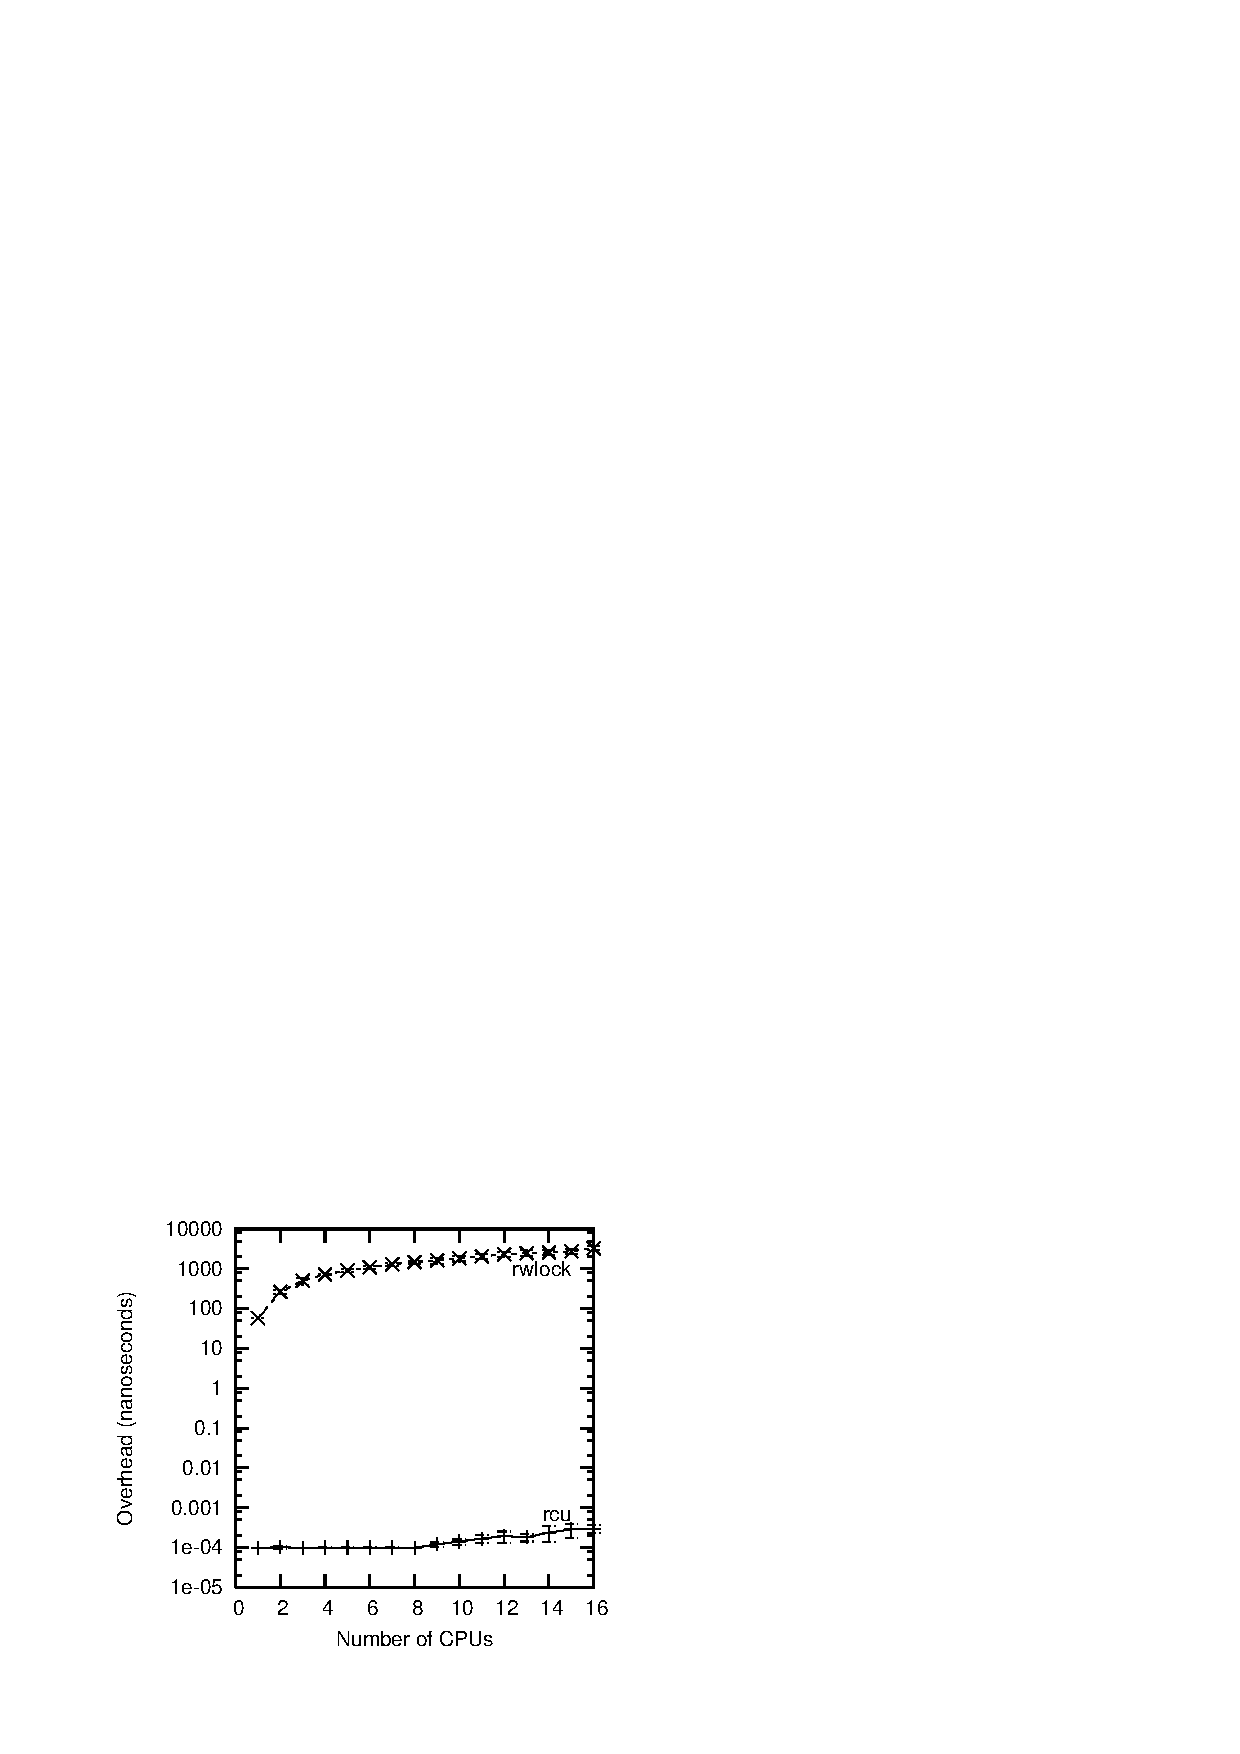
\includegraphics{CodeSamples/defer/data/rcuscale.hps.2020.05.28a/rwlockRCUperf}}
\caption{Performance Advantage of RCU Over Reader-Writer Locking}
\label{fig:defer:Performance Advantage of RCU Over Reader-Writer Locking}
\end{figure}

The read-side performance advantages of Linux-kernel RCU over
reader-writer locking are shown in
\cref{fig:defer:Performance Advantage of RCU Over Reader-Writer Locking},
which was generated on a 448-CPU 2.10\,GHz Intel x86 system.

\QuickQuizSeries{%
\QuickQuizB{
	WTF\@?
	How the heck do you expect me to believe that RCU can have less
	than a 300-picosecond overhead when the clock period at 2.10\,GHz
	is almost 500\,picoseconds?
}\QuickQuizAnswerB{
	First, consider that the inner loop used to
	take this measurement is as follows:

\begin{VerbatimN}
	for (i = nloops; i >= 0; i--) {
		rcu_read_lock();
		rcu_read_unlock();
	}
\end{VerbatimN}

	Next, consider the effective definitions of \co{rcu_read_lock()}
	and \co{rcu_read_unlock()}:

\begin{VerbatimN}
#define rcu_read_lock()   barrier()
#define rcu_read_unlock() barrier()
\end{VerbatimN}

	These definitions constrain compiler code-movement optimizations
	involving memory references, but emit no instructions in and
	of themselves.
	However, if the loop variable is maintained in a register,
	the accesses to \co{i} will not count as memory references.
	Furthermore, the compiler can do loop unrolling,
	allowing the resulting code to ``execute'' multiple passes
	through the loop body simply by incrementing \co{i} by
	some value larger than the value 1.

	So the ``measurement'' of 267 picoseconds is simply the fixed
	overhead of the timing measurements divided by the number of
	passes through the inner loop containing the calls
	to \co{rcu_read_lock()} and \co{rcu_read_unlock()}, plus
	the code to manipulate \co{i} divided by the loop-unrolling
	factor.
	And therefore, this measurement really is in error, in fact,
	it exaggerates the overhead by an arbitrary number of orders
	of magnitude.
	After all, in terms of machine instructions emitted, the actual
	overheads of \co{rcu_read_lock()} and of \co{rcu_read_unlock()}
	are each precisely zero.

	It is not just every day that a timing measurement of 267
	picoseconds turns out to be an overestimate!
}\QuickQuizEndB

\QuickQuizM{
	Didn't an earlier edition of this book show RCU read-side
	overhead way down in the sub-picosecond range?
	What happened???
}\QuickQuizAnswerM{
	Excellent memory!!!
	The overhead in some early releases was in fact roughly
	100~femtoseconds.

	What happened was that RCU usage spread more broadly through the
	Linux kernel, including into code that takes page faults.
	Back at that time, \co{rcu_read_lock()} and \co{rcu_read_unlock()}
	were complete no-ops in \co{CONFIG_PREEMPT=n} kernels.
	Unfortunately, that situation allowed the compiler to reorder
	page-faulting memory accesses into RCU read-side critical
	sections.
	Of course, page faults can block, which destroys those critical
	sections.

	Nor was this a theoretical problem:
	A failure actually manifested in 2019.
	\ppl{Herbert}{Xu} tracked down this failure down and
	\ppl{Linus}{Torvalds}
	therefore queued a commit to upgrade \co{rcu_read_lock()} and
	\co{rcu_read_unlock()} to unconditionally include a call to
	\co{barrier()}~\cite{LinusTorvalds2019:RCUreader.barrier}.
	And although \co{barrier()} emits no code, it does constrain
	compiler optimizations.
	And so the price of widespread RCU usage is slightly higher
	\co{rcu_read_lock()} and \co{rcu_read_unlock()} overhead.
	As such, Linux-kernel RCU has proven to be a victim of its
	own success.

	Of course, it is also the case that the older results were obtained
	on a different system than were those shown in
	\cref{fig:defer:Performance Advantage of RCU Over Reader-Writer Locking}.
	So which change had the most effect, Linus's commit or the change in
	the system?
	This question is left as an exercise to the reader.
}\QuickQuizEndM

\QuickQuizE{
	Why is there such large variation for the \co{RCU} trace in
	\cref{fig:defer:Performance Advantage of RCU Over Reader-Writer Locking}?
}\QuickQuizAnswerE{
	Keep in mind that this is a log-log plot, so those large-seeming
	\co{RCU} variances in reality span only a few hundred picoseconds.
	And that is such a short time that anything could cause it.
	However, given that the variance decreases with both small and
	large numbers of CPUs, one hypothesis is that the variation is
	due to migrations from one CPU to another.

	Yes, these measurements were taken with interrupts disabled, but
	they were also taken within a guest OS, so that preemption was
	still possible at the hypervisor level.
	In addition, the system featured hyperthreading and a single
	hardware thread running this RCU workload is able to consume
	more than half of the core's resources.
	Therefore, the overall throughput varies depending on how many
	of a given guest OS's CPUs share cores.
	Attempting to reduce these variations by running the guest OSes
	at real-time priority (as suggested by Joel Fernandes) is left
	as an exercise for the reader.
}\QuickQuizEndE
}                 % End of \QuickQuizSeries

Note that reader-writer locking is more than an order of magnitude slower
than RCU on a single CPU, and is more than \emph{four} orders of magnitude
slower on 192~CPUs.
In contrast, RCU scales quite well.
In both cases, the error bars cover the full range of the measurements
from 30~runs, with the line being the median.

\begin{figure}
\centering
\resizebox{2.5in}{!}{\includegraphics{CodeSamples/defer/data/rcuscale.hps.2020.05.28a/rwlockRCUperfPREEMPT}}
\caption{Performance Advantage of Preemptible RCU Over Reader-Writer Locking}
\label{fig:defer:Performance Advantage of Preemptible RCU Over Reader-Writer Locking}
\end{figure}

A more moderate view may be obtained from a \co{CONFIG_PREEMPT} kernel,
though RCU still beats reader-writer locking by between a factor of seven
on a single CPU and by three orders of magnitude on 192~CPUs, as shown in
\cref{fig:defer:Performance Advantage of Preemptible RCU Over Reader-Writer Locking},
which was generated on the same 448-CPU 2.10\,GHz x86 system.
Note the high variability of reader-writer locking at larger numbers of CPUs.
The error bars span the full range of data.

\QuickQuiz{
	Given that the system had no fewer than 448~hardware threads,
	why only 192~CPUs?
}\QuickQuizAnswer{
	Because the script (\path{rcuscale.sh}) that generates this data
	spawns a guest operating system for each set of points gathered,
	and on this particular system, both \co{qemu} and KVM limit the
	number of CPUs that may be configured into a given guest OS\@.
	Yes, it would have been possible to run a few more CPUs, but
	192 is a nice round number from a binary perspective, given
	that 256 is infeasible.
}\QuickQuizEnd

\begin{figure}
\centering
\resizebox{2.5in}{!}{\includegraphics{CodeSamples/defer/data/rcuscale.hps.2020.05.28a/rwlockRCUperfwt}}
\caption{Comparison of RCU to Reader-Writer Locking as Function of Critical-Section Duration, 192 CPUs}
\label{fig:defer:Comparison of RCU to Reader-Writer Locking as Function of Critical-Section Duration}
\end{figure}

Of course, the low performance of reader-writer locking in
\cref{fig:defer:Performance Advantage of RCU Over Reader-Writer Locking,%
fig:defer:Performance Advantage of Preemptible RCU Over Reader-Writer Locking}
is exaggerated by the unrealistic zero-length critical sections.
The performance advantages of RCU decrease as the overhead of the critical
sections increase, as shown in
\cref{fig:defer:Comparison of RCU to Reader-Writer Locking as Function of Critical-Section Duration},
which was run on the same system as the previous plots.
Here, the y-axis represents the sum of the overhead of the read-side
primitives and that of the critical section and the x-axis represents
the critical-section overhead in nanoseconds.
But please note the logscale y~axis, which means that the small
separations between the traces still represent significant differences.
This figure shows non-preemptible RCU, but given that preemptible RCU's
read-side overhead is only about three nanoseconds, its plot would be
nearly identical to
\cref{fig:defer:Comparison of RCU to Reader-Writer Locking as Function of Critical-Section Duration}.

\QuickQuiz{
	Why the larger error ranges for the submicrosecond durations in
	\cref{fig:defer:Comparison of RCU to Reader-Writer Locking as Function of Critical-Section Duration}?
}\QuickQuizAnswer{
	Because smaller disturbances result in greater relative errors
	for smaller measurements.
	Also, the Linux kernel's \co{ndelay()} nanosecond-scale primitive
	is (as of 2020) less accurate than is the \co{udelay()} primitive
	used for the data for durations of a microsecond or more.
	It is instructive to compare to the zero-length case shown in
	\cref{fig:defer:Performance Advantage of RCU Over Reader-Writer Locking}.
}\QuickQuizEnd

There are three traces for reader-writer locking, with the upper trace
being for 100~CPUs, the next for 10~CPUs, and the lowest for 1~CPU\@.
The greater the number of CPUs and the shorter the critical sections,
the greater is RCU's performance advantage.
These performance advantages are underscored by the fact that 100-CPU
systems are no longer uncommon and that a number of system calls (and
thus any RCU read-side critical sections that they contain) complete
within microseconds.

In addition, as is discussed in the next section,
RCU read-side primitives are almost entirely deadlock-immune.


\paragraph{Deadlock Immunity}

Although RCU offers significant performance advantages for
read-mostly workloads, one of the primary reasons for creating
RCU in the first place was in fact its immunity to read-side
deadlocks.
This immunity stems from the fact that
RCU read-side primitives do not block, spin, or even
do backwards branches, so that their execution time is deterministic.
It is therefore impossible for them to participate in a deadlock
cycle.

\QuickQuiz{
	Is there an exception to this deadlock immunity, and if so,
	what sequence of events could lead to deadlock?
}\QuickQuizAnswer{
	One way to cause a deadlock cycle involving
	RCU read-side primitives is via the following (illegal) sequence
	of statements:

\begin{VerbatimU}
rcu_read_lock();
synchronize_rcu();
rcu_read_unlock();
\end{VerbatimU}

	The \co{synchronize_rcu()} cannot return until all
	pre-existing RCU read-side critical sections complete, but
	is enclosed in an RCU read-side critical section that cannot
	complete until the \co{synchronize_rcu()} returns.
	The result is a classic self-deadlock---you get the same
	effect when attempting to write-acquire a reader-writer lock
	while read-holding it.

	Note that this self-deadlock scenario does not apply to
	RCU QSBR, because the context switch performed by the
	\co{synchronize_rcu()} would act as a quiescent state
	for this CPU, allowing a grace period to complete.
	However, this is if anything even worse, because data used
	by the RCU read-side critical section might be freed as a
	result of the grace period completing.
	Plus Linux kernel's lockdep facility will yell at you.

	In short, do not invoke synchronous RCU update-side primitives
	from within an RCU read-side critical section.

	In addition, within the Linux kernel, RCU uses the scheduler
	and the scheduler uses RCU\@.
	In some cases, both RCU and the scheduler must take care to
	avoid deadlock.
}\QuickQuizEnd

An interesting consequence of RCU's read-side deadlock immunity is
that it is possible to unconditionally upgrade an RCU
reader to an RCU updater.
Attempting to do such an upgrade with reader-writer locking results
in deadlock.
A sample code fragment that does an RCU read-to-update upgrade follows:

\begin{VerbatimN}[samepage=true]
rcu_read_lock();
list_for_each_entry_rcu(p, &head, list_field) {
	do_something_with(p);
	if (need_update(p)) {
		spin_lock(my_lock);
		do_update(p);
		spin_unlock(&my_lock);
	}
}
rcu_read_unlock();
\end{VerbatimN}

Note that \co{do_update()} is executed under
the protection of the lock \emph{and} under RCU read-side protection.

Another interesting consequence of RCU's deadlock immunity is its
immunity to a large class of priority inversion problems.
For example, low-priority RCU readers cannot prevent a high-priority
RCU updater from acquiring the update-side lock.
Similarly, a low-priority RCU updater cannot prevent high-priority
RCU readers from entering an RCU read-side critical section.

\QuickQuiz{
	Immunity to both deadlock and priority inversion???
	Sounds too good to be true.
	Why should I believe that this is even possible?
}\QuickQuizAnswer{
	It really does work.
	After all, if it didn't work, the Linux kernel would not run.
}\QuickQuizEnd

\paragraph{Realtime Latency}

Because RCU read-side primitives neither spin nor block, they offer
excellent realtime latencies.
In addition, as noted earlier, this means that they are
immune to priority inversion
involving the RCU read-side primitives and locks.

However, RCU is susceptible to more subtle priority-inversion scenarios,
for example, a high-priority process blocked waiting for an RCU
grace period to elapse can be blocked by low-priority RCU readers
in \rt\ kernels.
This can be solved by using RCU priority
boosting~\cite{PaulEMcKenney2007BoostRCU,DinakarGuniguntala2008IBMSysJ}.

However, use of RCU priority boosting requires that \co{rcu_read_unlock()}
do deboosting, which entails acquiring scheduler locks.
Some care is therefore required within the scheduler and RCU to avoid
deadlocks, which as of the v5.15 Linux kernel requires RCU to avoid
invoking the scheduler while holding any of RCU's locks.

This in turn means that \co{rcu_read_unlock()} is not always lockless
when RCU priority boosting is enabled.
However, \co{rcu_read_unlock()} will still be lockless if its
critical section was not priority-boosted.
Furthermore, critical sections will not be priority boosted unless they
are preempted, or, in -rt kernels, they acquire non-raw spinlocks.
This means that \co{rcu_read_unlock()} will normally be lockless from the
perspective of the highest priority task running on any given CPU.

\paragraph{RCU Readers and Updaters Run Concurrently}

Because RCU readers never spin nor block, and because updaters are not
subject to any sort of rollback or abort semantics, RCU readers and
updaters really can run concurrently.
This means that RCU readers might access stale data, and might even
see inconsistencies, either of which can render conversion from reader-writer
locking to RCU non-trivial.

\begin{figure}
\centering
\resizebox{3in}{!}{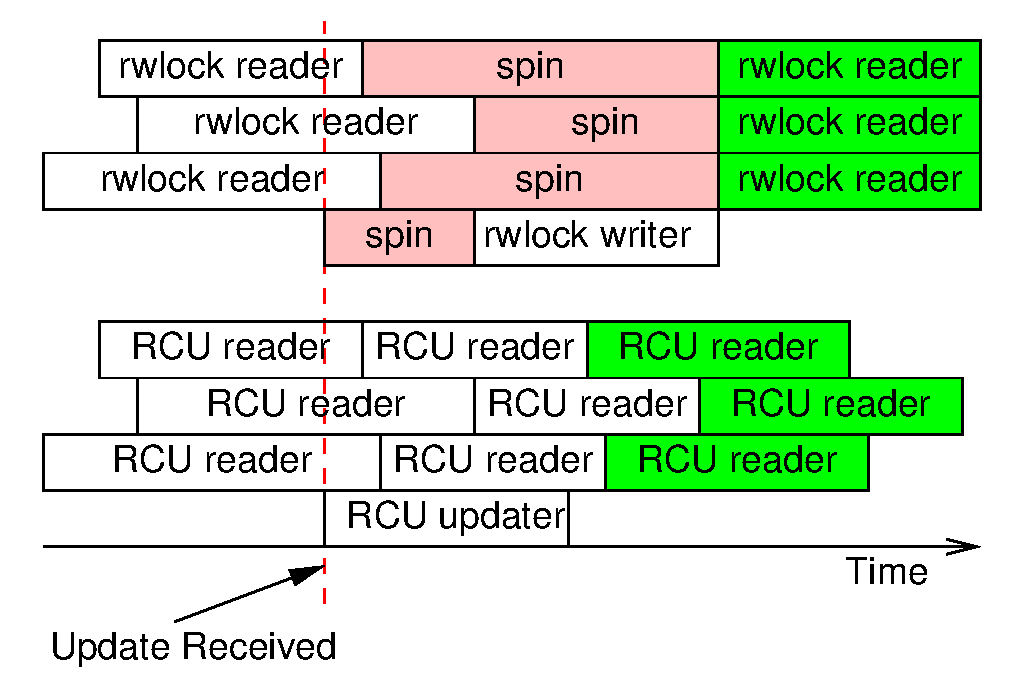
\includegraphics{defer/rwlockRCUupdate}}
\caption{Response Time of RCU vs.\@ Reader-Writer Locking}
\label{fig:defer:Response Time of RCU vs. Reader-Writer Locking}
\end{figure}

However, in a surprisingly large number of situations, inconsistencies and
stale data are not problems.
The classic example is the networking routing table.
Because routing updates can take considerable time to reach a given
system (seconds or even minutes), the system will have been sending
packets the wrong way for quite some time when the update arrives.
It is usually not a problem to continue sending updates the wrong
way for a few additional milliseconds.
Furthermore, because RCU updaters can make changes without waiting for
RCU readers to finish,
the RCU readers might well see the change more quickly than would
batch-fair
reader-writer-locking readers, as shown in
\cref{fig:defer:Response Time of RCU vs. Reader-Writer Locking}.

\QuickQuiz{
	But how many other algorithms really tolerate stale and
	inconsistent data?
}\QuickQuizAnswer{
	Quite a few!

	Please keep in mind that the finite speed of light means that
	data reaching a given computer system is at least slightly stale
	at the time that it arrives, and extremely stale in the case
	of astronomical data.
	The finite speed of light also places a sharp limit on the
	consistency of data arriving from different sources of via
	different paths.

	You might as well face the fact that the laws of physics
	are incompatible with naive notions of perfect freshness and
	consistency.
}\QuickQuizEnd

Once the update is received, the rwlock writer cannot proceed until the
last reader completes, and subsequent readers cannot proceed until the
writer completes.
However, these subsequent readers are guaranteed to see the new value,
as indicated by the green shading of the rightmost boxes.
In contrast, RCU readers and updaters do not block each other, which permits
the RCU readers to see the updated values sooner.
Of course, because their execution overlaps that of the RCU updater,
\emph{all} of the RCU readers might well see updated values, including
the three readers that started before the update.
Nevertheless only the green-shaded rightmost RCU readers
are \emph{guaranteed} to see the updated values.

Reader-writer locking and RCU simply provide different guarantees.
With reader-writer locking, any reader that begins after the writer begins
is guaranteed to see new values, and any reader that attempts to
begin while the writer is spinning might or might not see new values,
depending on the reader/writer preference of the rwlock implementation in
question.
In contrast, with RCU, any reader that begins after the updater completes
is guaranteed to see new values, and any reader that completes after the
updater begins might or might not see new values, depending on timing.

The key point here is that, although reader-writer locking does
indeed guarantee consistency within the confines of the computer system,
there are situations where this consistency comes at the price of
increased \emph{inconsistency} with the outside world, courtesy of
the finite speed of light and the non-zero size of atoms.
In other words, reader-writer locking obtains internal consistency at the
price of silently stale data with respect to the outside world.

Note that if a value is computed while read-holding a reader-writer
lock, and then that value is used after that lock is released, then
this reader-writer-locking use case is using stale data.
After all, the quantities that this value is based on could change
at any time after that lock is released.
This sort of reader-writer-locking use case is often easy to
convert to RCU, as will be shown in
\cref{lst:defer:Converting Reader-Writer Locking to RCU: Data,%
lst:defer:Converting Reader-Writer Locking to RCU: Search,%
lst:defer:Converting Reader-Writer Locking to RCU: Deletion}
and the accompanying text.

\paragraph{Low-Priority RCU Readers Can Block High-Priority Reclaimers}

In Realtime RCU~\cite{DinakarGuniguntala2008IBMSysJ} or
SRCU~\cite{PaulEMcKenney2006c},
a preempted reader will prevent a grace period from completing, even if
a high-priority task is blocked waiting for that grace period to complete.
Realtime RCU can avoid this problem by substituting \co{call_rcu()}
for \co{synchronize_rcu()} or by using RCU priority
boosting~\cite{PaulEMcKenney2007BoostRCU,DinakarGuniguntala2008IBMSysJ}.
It might someday be necessary to augment SRCU and RCU Tasks Trace with
priority boosting, but not before a clear real-world need is demonstrated.

\QuickQuiz{
	If Tasks RCU Trace might someday be priority boosted, why
	not also Tasks RCU and Tasks RCU Rude?
}\QuickQuizAnswer{
	Maybe, but these are less likely.

	In the case of Tasks RCU, recall that the quiescent state is
	a voluntary context switch.
	Thus, all tasks not blocked after a voluntary context switch
	might need to be boosted, and the mechanics of deboosting would
	not likely be at all pretty.

	In the case of Tasks RCU Rude, as was the case with the old
	RCU Sched, any preemptible region of code is a quiescent state.
	Thus, the only tasks that might need boosting are those currently
	running with preemption disabled.
	But boosting the priority of a preemption-disabled task has no
	effect.
	It therefore seems doubly unlikely that priority boosting will
	ever be introduced to Tasks RCU Rude, at least in its current
	form.
}\QuickQuizEnd

\paragraph{RCU Grace Periods Extend for Many Milliseconds}

With the exception of userspace
RCU~\cite{MathieuDesnoyers2009URCU,PaulMcKenney2013LWNURCU},
expedited grace periods, and several of the ``toy''
RCU implementations described in
\cref{chp:app:``Toy'' RCU Implementations},
RCU grace periods extend milliseconds.
Although there are a number of techniques to render such long
delays harmless, including use of the asynchronous interfaces
(\co{call_rcu()} and \co{call_rcu_bh()}) or of the polling interfaces
(\co{get_state_synchronize_rcu()}, \co{start_poll_synchronize_rcu()},
and \co{poll_state_synchronize_rcu()}), this situation is a major reason
for the rule of thumb that RCU be used in read-mostly situations.

As noted in \cref{sec:defer:RCU Linux-Kernel API}, within the Linux
kernel, shorter grace periods may be obtained via expedited grace
periods, for example, by invoking \co{synchronize_rcu_expedited()}
instead of \co{synchronize_rcu()}.
Expedited grace periods can reduce delays to as little as a few tens of
microseconds, albeit at the expense of higher CPU utilization and IPIs.
The added IPIs can be especially unwelcome in some real-time workloads.

\paragraph{Code:
		 Reader-Writer Locking vs.\@ RCU}

In the best case, the conversion from reader-writer locking to RCU
is quite simple, as shown in
\cref{lst:defer:Converting Reader-Writer Locking to RCU: Data,%
lst:defer:Converting Reader-Writer Locking to RCU: Search,%
lst:defer:Converting Reader-Writer Locking to RCU: Deletion},
all taken from
Wikipedia~\cite{WikipediaRCU}.

\begin{listing*}
{ \scriptsize
\begin{verbbox}
 1 struct el {                           1 struct el {
 2   struct list_head lp;                2   struct list_head lp;
 3   long key;                           3   long key;
 4   spinlock_t mutex;                   4   spinlock_t mutex;
 5   int data;                           5   int data;
 6   /* Other data fields */             6   /* Other data fields */
 7 };                                    7 };
 8 DEFINE_RWLOCK(listmutex);             8 DEFINE_SPINLOCK(listmutex);
 9 LIST_HEAD(head);                      9 LIST_HEAD(head);
\end{verbbox}
}
\hspace*{0.9in}\OneColumnHSpace{-0.5in}
\IfEbookSize{\hspace*{-1.05in}}{}\theverbbox
\caption{Converting Reader-Writer Locking to RCU\@:
						    Data}
\label{lst:defer:Converting Reader-Writer Locking to RCU: Data}
\end{listing*}

\begin{listing*}
{ \scriptsize
\begin{verbbox}
 1 int search(long key, int *result)     1 int search(long key, int *result)
 2 {                                     2 {
 3   struct el *p;                       3   struct el *p;
 4                                       4
 5   read_lock(&listmutex);              5   rcu_read_lock();
 6   list_for_each_entry(p, &head, lp) { 6   list_for_each_entry_rcu(p, &head, lp) {
 7     if (p->key == key) {              7     if (p->key == key) {
 8       *result = p->data;              8       *result = p->data;
 9       read_unlock(&listmutex);        9       rcu_read_unlock();
10       return 1;                      10       return 1;
11     }                                11     }
12   }                                  12   }
13   read_unlock(&listmutex);           13   rcu_read_unlock();
14   return 0;                          14   return 0;
15 }                                    15 }
\end{verbbox}
}
\hspace*{0.9in}\OneColumnHSpace{-0.5in}
\IfEbookSize{\hspace*{-1.05in}}{}\theverbbox
\caption{Converting Reader-Writer Locking to RCU\@:
						    Search}
\label{lst:defer:Converting Reader-Writer Locking to RCU: Search}
\end{listing*}

\begin{listing*}
{ \scriptsize
\begin{verbbox}
 1 int delete(long key)                  1 int delete(long key)
 2 {                                     2 {
 3   struct el *p;                       3   struct el *p;
 4                                       4
 5   write_lock(&listmutex);             5   spin_lock(&listmutex);
 6   list_for_each_entry(p, &head, lp) { 6   list_for_each_entry(p, &head, lp) {
 7     if (p->key == key) {              7     if (p->key == key) {
 8       list_del(&p->lp);               8       list_del_rcu(&p->lp);
 9       write_unlock(&listmutex);       9       spin_unlock(&listmutex);
                                        10       synchronize_rcu();
10       kfree(p);                      11       kfree(p);
11       return 1;                      12       return 1;
12     }                                13     }
13   }                                  14   }
14   write_unlock(&listmutex);          15   spin_unlock(&listmutex);
15   return 0;                          16   return 0;
16 }                                    17 }
\end{verbbox}
}
\hspace*{0.9in}\OneColumnHSpace{-0.5in}
\IfEbookSize{\hspace*{-1.05in}}{}\theverbbox
\caption{Converting Reader-Writer Locking to RCU\@:
						    Deletion}
\label{lst:defer:Converting Reader-Writer Locking to RCU: Deletion}
\end{listing*}

However, the transformation is not always this straightforward.
This is because neither the \co{spin_lock()} nor the
\co{synchronize_rcu()} in
\cref{lst:defer:Converting Reader-Writer Locking to RCU: Deletion}
exclude the readers in
\cref{lst:defer:Converting Reader-Writer Locking to RCU: Search}.
First, the \co{spin_lock()} does not interact in any way with
\co{rcu_read_lock()} and \co{rcu_read_unlock()}, thus not excluding them.
Second, although both \co{write_lock()} and \co{synchronize_rcu()}
wait for pre-existing readers, only \co{write_lock()} prevents
subsequent readers from commencing.\footnote{
	Kudos to whoever pointed this out to Paul.}
Thus, \co{synchronize_rcu()} cannot exclude readers.
It is therefore surprising that a great many situations
using reader-writer locking can be easily converted to RCU\@.

More-elaborate cases of replacing reader-writer locking with RCU
may be found
elsewhere~\cite{NeilBrown2015PathnameLookup,NeilBrown2015RCUwalk}.

\paragraph{Semantics:
		      Reader-Writer Locking vs.\@ RCU}

Reader-writer locking semantics can be roughly and informally summarized
by the following three temporal constraints:

\begin{enumerate}
\item	Write-side acquisitions wait for any read-holders to release
	the lock.
\item	Writer-side acquisitions wait for any write-holder to release
	the lock.
\item	Read-side acquisitions wait for any write-holder to release
	the lock.
\end{enumerate}

RCU dispenses entirely with constraint~\#3 and weakens the other two
as follows:

\begin{enumerate}
\item	Writers wait for any pre-existing read-holders before progressing
	to the destructive phase of their update (usually the freeing of
	memory).
\item	Writers synchronize with each other as needed.
\end{enumerate}

It is of course this weakening that permits RCU implementations to attain
excellent performance and scalability.
It also allows RCU to implement the aforementioned unconditional
read-to-write upgrade that is so attractive and so deadlock-prone in
reader-writer locking.
Code using RCU can compensate for this weakening in a surprisingly large
number of ways, but most commonly by imposing spatial constraints:

\begin{enumerate}
\item	New data is placed in newly allocated memory.
\item	Old data is freed, but only after:
	\begin{enumerate}
	\item	That data has been unlinked so as to be inaccessible
		to later readers, and
	\item	A subsequent RCU grace period has elapsed.
	\end{enumerate}
\end{enumerate}

Of course, there are some reader-writer-locking use cases for which RCU's
weakened semantics are inappropriate, but experience in the Linux kernel
indicates that most reader-writer locks can in fact be replaced by RCU\@.
A surprisingly common case involves some value is computed while holding
the lock and then used after releasing that lock, and such cases can
frequently accommodate RCU's weaker semantics.

\begin{listing}
\input{CodeSamples/defer/singleton@get.fcv}
\caption{RCU Singleton Get}
\label{lst:defer:Singleton Get}
\end{listing}

\begin{listing}
\input{CodeSamples/defer/singleton@set.fcv}
\caption{RCU Singleton Set}
\label{lst:defer:Singleton Set}
\end{listing}

\begin{fcvref}[ln:defer:singleton:get]
This interaction of temporal and spatial constraints is illustrated
by the RCU singleton data structure illustrated in
\cref{fig:defer:Insertion With Concurrent Readers,fig:defer:Deletion With Concurrent Readers}.
This structure is defined on \clnrefrange{myconfig.b}{myconfig.e} of
\cref{lst:defer:Singleton Get}, and contains two integer fields,
\co{->a} and \co{->b} (\path{singleton.c}).
The current instance of this structure is referenced by the \co{curconfig}
pointer defined on \clnref{myconfig.e}.
\end{fcvref}

\begin{fcvref}[ln:defer:singleton:get]
The fields of the current structure are passed back through the
\co{cur_a} and \co{cur_b} parameters to the \co{get_config()} function
defined on \clnrefrange{get_config.b}{get_config.e}.
These two fields can be slightly out of date, but they absolutely must
be consistent with each other.
The \co{get_config()} function provides this consistency
within the RCU read-side critical section starting on
\clnref{rrl} and ending on either \clnref{rrul1} or \clnref{rrul2},
which provides the needed temporal synchronization.
\Clnref{rderef} fetches the pointer to the current \co{myconfig} structure.
This structure will be used regardless of any concurrent changes due
to calls to the \co{set_config()} function, thus providing the needed
spatial synchronization.
If \clnref{nullchk} determines that the \co{curconfig} pointer was
\co{NULL}, \clnref{retfail} returns failure.
Otherwise, \clnref{copya,copyb} copy out the \co{->a} and \co{->b} fields
and \clnref{retsuccess} returns success.
These \co{->a} and \co{->b} fields are from the same \co{myconfig}
structure, and the RCU read-side critical section prevents this structure
from being freed, thus guaranteeing that these two fields are consistent
with each other.
\end{fcvref}

\begin{fcvref}[ln:defer:singleton:set]
The structure is updated by the \co{set_config()} function shown in
\cref{lst:defer:Singleton Set}.
\Clnrefrange{allocinit.b}{allocinit.e} allocate and initialize a
new \co{myconfig} structure.
\Clnref{xchg} atomically exchanges a pointer to this new structure with
the pointer to the old structure in \co{curconfig}, while also providing
full memory ordering both before and after the \co{xchg()} operation,
thus providing the needed updater/reader spatial synchronization on
the one hand and the needed updater/updater synchronization on the other.
If \clnref{if} determines that the pointer to the old structure was
in fact non-\co{NULL}, \clnref{sr} waits for a grace period (thus providing
the needed reader/updater temporal synchronization) and \clnref{free}
frees the old structure, safe in the knowledge that there are no
longer any readers still referencing it.
\end{fcvref}

\begin{figure*}
\centering
\resizebox{\onecolumntextwidth}{!}{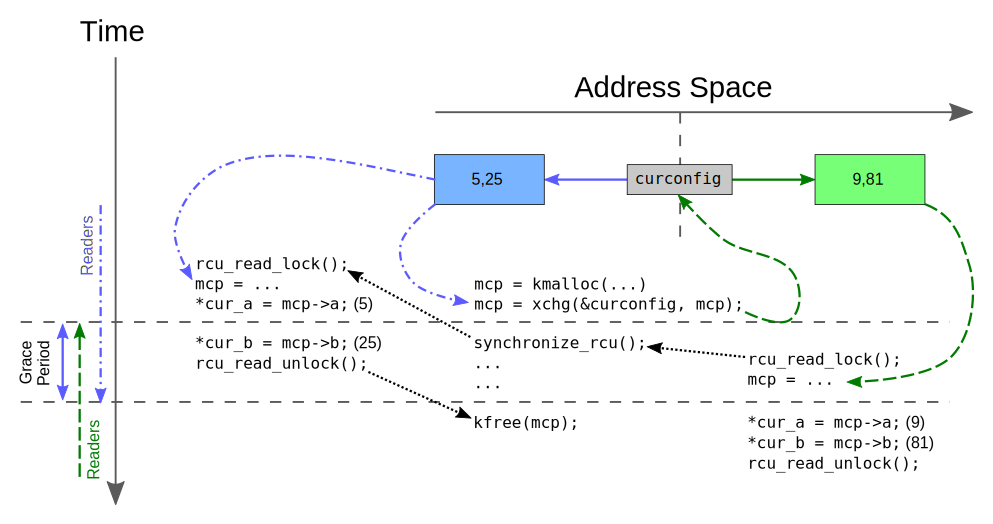
\includegraphics{defer/RCUspacetime}}
\caption{RCU Spatial/Temporal Synchronization}
\label{fig:defer:RCU Spatial/Temporal Synchronization}
\end{figure*}

\Cref{fig:defer:RCU Spatial/Temporal Synchronization} shows an abbreviated
representation of \co{get_config()} on the left and right and a similarly
abbreviated representation of \co{set_config()} in the middle.
Time advances from top to bottom, and the address space of the objects
referenced by \co{curconfig} advances from left to right.
The boxes with comma-separated numbers each represent a \co{myconfig}
structure, with the constraint that \co{->b} is the square of \co{->a}.
Each blue dash-dotted arrow represents an interaction with the old structure
(on the left, containing ``5,25'') and each green dashed arrow represents
an interaction with the new structure (on the right, containing ``9,81'').

The black dotted arrows represent temporal relationships between RCU readers
on the left and right and the RCU grace period at center, with each
arrow pointing from an older event to a newer event.
The call to \co{synchronize_rcu()} followed the leftmost \co{rcu_read_lock()},
and therefore that \co{synchronize_rcu()} invocation must not return
until after the corresponding \co{rcu_read_unlock()}.
In contrast, the call to \co{synchronize_rcu()} precedes the
rightmost \co{rcu_read_lock()}, which allows the return from that same
\co{synchronize_rcu()} to ignore the corresponding \co{rcu_read_unlock()}.
These temporal relationships prevent the \co{myconfig} structures from
being freed while RCU readers are still accessing them.

The two horizontal grey dashed lines represent the period of time during
which different readers get different results, however, each reader
will see one and only one of the two objects.
Before the first horizontal line, all readers see the leftmost
\co{myconfig} structure, and after the second horizontal line, all
readers will see the rightmost structure.
Between the two lines, that is, during the grace period, different
readers might see different objects, but as long as each reader
loads the \co{curconfig} pointer only once, each reader will see
a consistent view of its \co{myconfig} structure.

In short, RCU can approximate a reader-writer lock with the RCU read-side
critical section acting as the reader by combining temporal and spatial
synchronization, as shown in
\cref{fig:defer:Relationships Between RCU Use Cases,fig:defer:RCU Spatial/Temporal Synchronization}.

\subsubsection{Quasi Reference Count}
\label{sec:defer:Quasi Reference Count}

Because grace periods are not allowed to complete while
there is an RCU read-side critical section in progress,
the RCU read-side primitives may be used as a restricted
reference-counting mechanism.
For example, consider the following code fragment:

\begin{VerbatimN}
rcu_read_lock();  /* acquire reference. */
p = rcu_dereference(head);
/* do something with p. */
rcu_read_unlock();  /* release reference. */
\end{VerbatimN}

The combination of the \co{rcu_read_lock()} and \co{rcu_dereference()}
primitives can be thought of as acquiring a reference to \co{p},
because a grace period starting after the \co{rcu_dereference()}
assignment to \co{p} cannot possibly end until after we reach the matching
\co{rcu_read_unlock()}.
This reference-counting scheme is restricted in that
we are not allowed to block in RCU read-side critical sections,
nor are we permitted to hand off an RCU read-side critical section's
references from one task to another.

Regardless of these restrictions,
the following code can safely delete \co{p}:

\begin{VerbatimN}
spin_lock(&mylock);
p = head;
rcu_assign_pointer(head, NULL);
spin_unlock(&mylock);
/* Wait for all references to be released. */
synchronize_rcu();
kfree(p);
\end{VerbatimN}

The assignment to \co{head} prevents any future references
to \co{p} from being acquired, and the \co{synchronize_rcu()}
waits for any previously acquired references to be released.

\QuickQuiz{
	But wait!
	This is exactly the same code that might be used when thinking
	of RCU as a replacement for reader-writer locking!
	What gives?
}\QuickQuizAnswer{
	This is an effect of the Law of Toy Examples:
	Beyond a certain point, the code fragments look the same.
	The only difference is in how we think about the code.
	For example, what does an \co{atomic_inc()} operation do?
	It might be acquiring another explicit reference to an object
	to which we already have a reference, it might be incrementing
	an often-read/seldom-updated statistical counter, it might
	be checking into an HPC-style barrier, or any of a number of
	other things.

	However, these differences can be extremely important.
	For but one example of the importance, consider that if we think
	of RCU as a restricted reference counting scheme, we would never
	be fooled into thinking that the updates would exclude the RCU
	read-side critical sections.

	It nevertheless is often useful to think of RCU as a replacement
	for reader-writer locking, for example, when you are replacing
	reader-writer locking with RCU\@.
}\QuickQuizEnd

Of course, RCU can also be combined with traditional reference counting,
as discussed in
\cref{sec:together:Refurbish Reference Counting}.

\begin{figure}
\centering
\resizebox{2.5in}{!}{\includegraphics{CodeSamples/defer/data/rcuscale.hps.2020.05.28a/refcntRCUperf}}
\caption{Performance of RCU vs.\@ Reference Counting}
\label{fig:defer:Performance of RCU vs. Reference Counting}
\end{figure}

\begin{figure}
\centering
\resizebox{2.5in}{!}{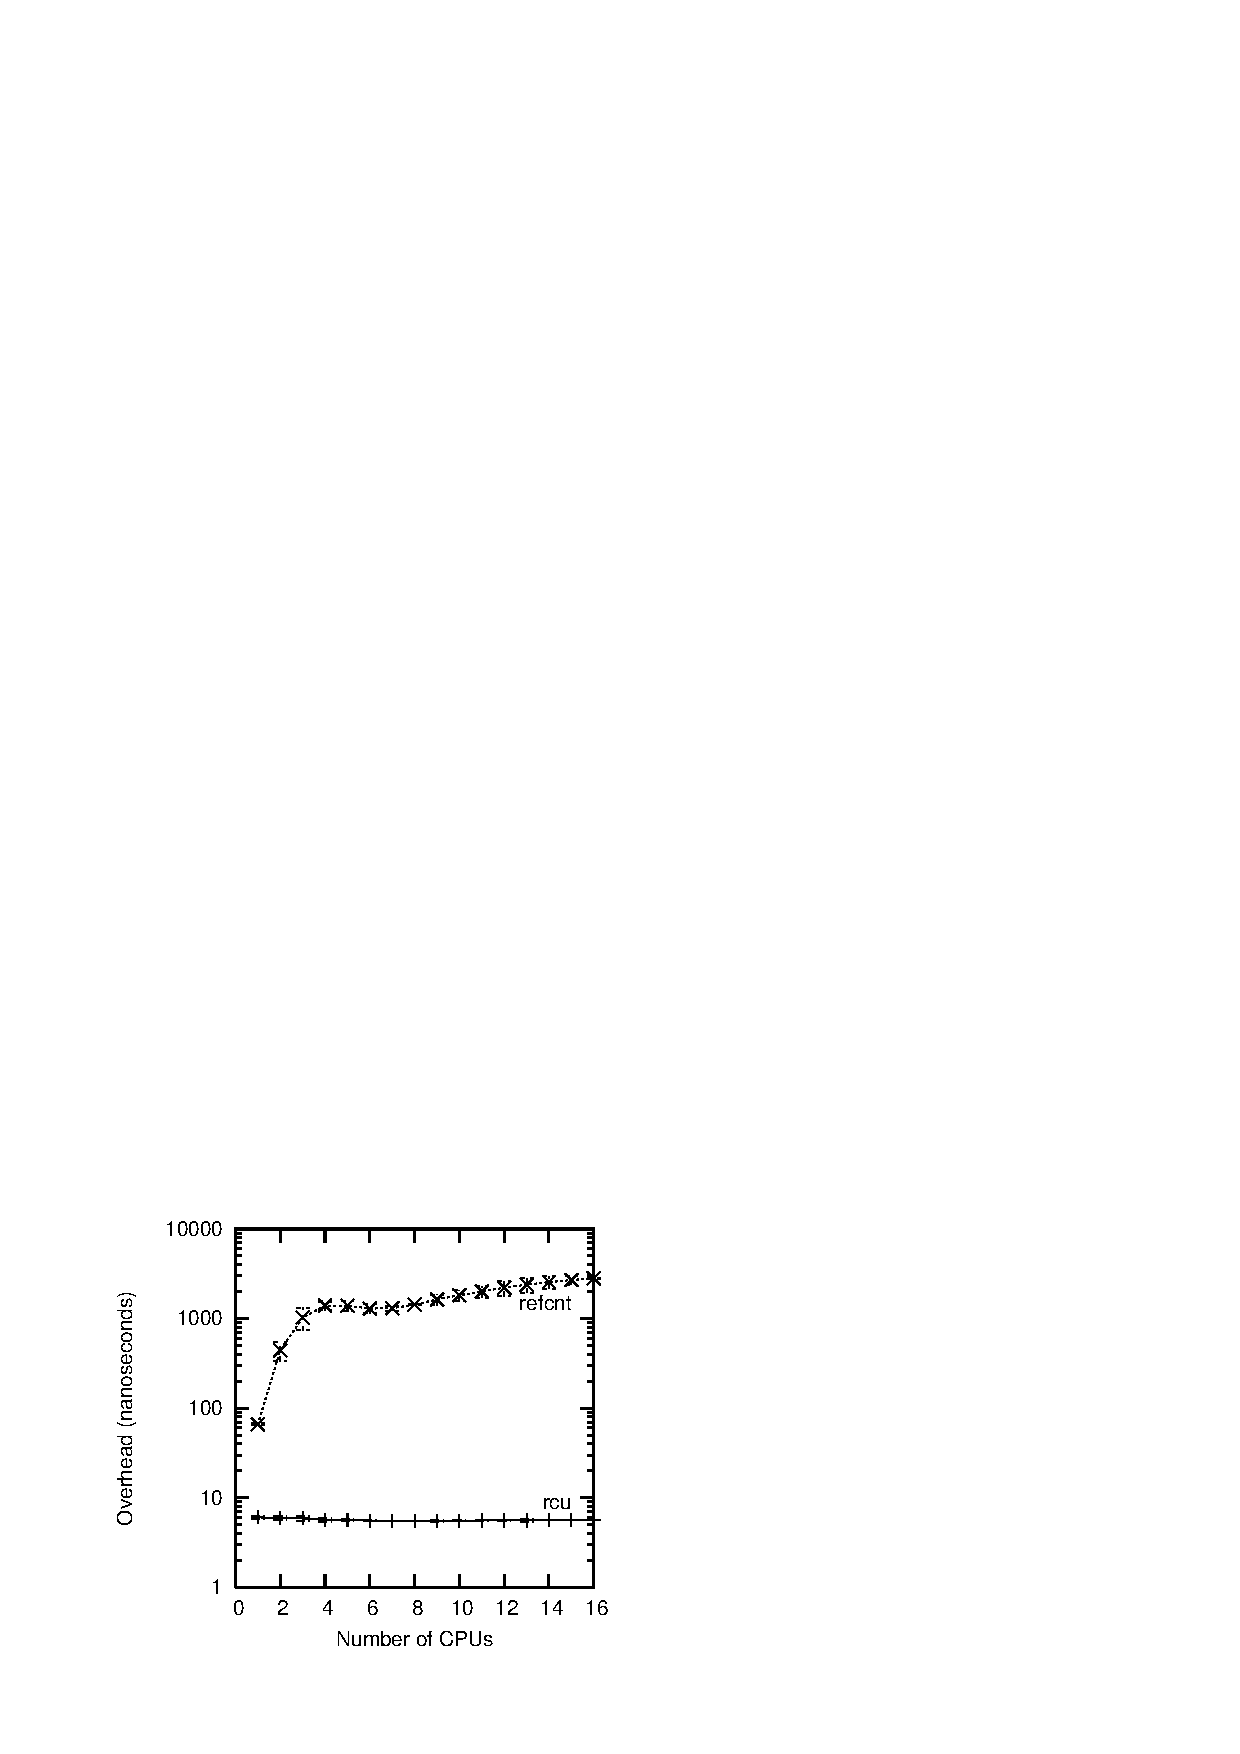
\includegraphics{CodeSamples/defer/data/rcuscale.hps.2020.05.28a/refRCUperfPREEMPT}}
\caption{Performance of Preemptible RCU vs.\@ Reference Counting}
\label{fig:defer:Performance of Preemptible RCU vs. Reference Counting}
\end{figure}

But why bother?
Again, part of the answer is performance, as shown in
\cref{fig:defer:Performance of RCU vs. Reference Counting,%
fig:defer:Performance of Preemptible RCU vs. Reference Counting},
again showing data taken on a 448-CPU 2.1\,GHz Intel x86 system
for non-preemptible and preemptible Linux-kernel RCU, respectively.
Non-preemptible RCU's advantage over
\IXalt{reference counting}{reference count} ranges from
more than an order of magnitude at one CPU up to about four orders of
magnitude at 192~CPUs.
Preemptible RCU's advantage ranges from about a factor of three at
one CPU up to about three orders of magnitude at 192~CPUs.

\begin{figure}
\centering
\resizebox{2.5in}{!}{\includegraphics{CodeSamples/defer/data/rcuscale.hps.2020.05.28a/refRCUperfwt}}
\caption{Response Time of RCU vs.\@ Reference Counting, 192 CPUs}
\label{fig:defer:Response Time of RCU vs. Reference Counting}
\end{figure}

However, as with reader-writer locking, the performance advantages of
RCU are most pronounced for short-duration critical sections and for
large numbers of CPUs, as shown in
\cref{fig:defer:Response Time of RCU vs. Reference Counting}
for the same system.
In addition, as with reader-writer locking, many system calls (and thus
any RCU read-side critical sections that they contain) complete in
a few microseconds.

Although traditional reference counters are usually associated with a
specific data structure, or perhaps a specific group of data structures,
this approach does have some disadvantages.
For example, maintaining a single global reference counter for a large
variety of data structures typically results in bouncing the cache line
containing the reference count.
As we saw in
\crefrange{fig:defer:Performance of RCU vs. Reference Counting}{fig:defer:Response Time of RCU vs. Reference Counting},
such cache-line bouncing can severely degrade performance.

In contrast, RCU's lightweight \co{rcu_read_lock()},
\co{rcu_dereference()}, and \co{rcu_read_unlock()} read-side primitives
permit extremely frequent read-side usage with negligible performance
degradation.
Except that the calls to \co{rcu_dereference()} are not doing anything
specific to acquire a reference to the pointed-to object.
The heavy lifting is instead done by the \co{rcu_read_lock()} and
\co{rcu_read_unlock()} primitives and their interactions with RCU
grace periods.

And ignoring those calls to \co{rcu_dereference()} permits RCU to be
thought of as a ``bulk reference-counting'' mechanism, where each call
to \co{rcu_read_lock()} obtains a reference on each and every RCU-protected
object, and with little or no overhead.
However, the restrictions that go with RCU can be quite onerous.
For example, in many cases, the prohibition against sleeping while in an RCU
read-side critical section would defeat the entire purpose.
Such cases might be better served by the hazard pointers mechanism
described in \cref{sec:defer:Hazard Pointers}.
Cases where code rarely sleeps have been handled by using RCU as a
reference count in the common non-sleeping case and by bridging
to an explicit reference counter when sleeping is necessary.

Alternatively, situations where a reference must be held by a single task
across a section of code that sleeps may be accommodated with Sleepable
RCU (SRCU)~\cite{PaulEMcKenney2006c}.
This fails to cover the not-uncommon situation where a reference is ``passed''
from one task to another, for example, when a reference is acquired
when starting an I/O and released in the corresponding completion
interrupt handler.
Again, such cases might be better handled by explicit reference counters
or by hazard pointers.

Of course, SRCU brings restrictions of its own, namely that the
return value from \co{srcu_read_lock()} be passed into the
corresponding \co{srcu_read_unlock()}, and that no SRCU primitives
be invoked from hardware interrupt handlers or from \IXacrf{nmi}
handlers.
The jury is still out as to how much of a problem is presented by
this restriction, and as to how it can best be handled.

However, in the common case where references are held within the confines
of a single CPU or task, RCU can be used as high-performance and highly
scalable reference-counting mechanism.

As shown in \cref{fig:defer:Relationships Between RCU Use Cases},
quasi reference counts add RCU readers as individual or bulk
reference counts, possibly also bridging to reference counters
in corner cases.

\subsubsection{Quasi Multi-Version Concurrency Control}
\label{sec:defer:Quasi Multi-Version Concurrency Control}

RCU can also be thought of as a simplified multi-version concurrency
control (MVCC) mechanism with weak consistency criteria.
The multi-version aspects were touched upon in
\cref{sec:defer:Maintain Multiple Versions of Recently Updated Objects}.
However, in its native form, RCU provides version consistency only
within a given RCU-protected data element.

Nevertheless, there are situations where inconsistency and stale
data within the broader confines of the system cannot be tolerated.
Fortunately, there are a number of approaches that avoid inconsistency
and stale data, including the following:

\begin{enumerate}
\item	RCU readers can be enclosed in sequence-locking readers, forcing
	the RCU readers to be retried should an update occur,
	as described in
	\cref{sec:together:Correlated Data Elements}
	and
	\cref{sec:together:Atomic Move}.
\item	Place the data that must be consistent into a single element
	of a linked data structure, and refrain from updating those
	fields within any element visible to RCU readers.
	RCU readers gaining a reference to any such element are then
	guaranteed to see consistent values.
	See \cref{sec:together:Correlated Fields} for additional details.
\item	Use a per-element lock that guards a ``deleted'' flag to allow
	RCU readers to reject stale
	data~\cite{PaulEdwardMcKenneyPhD,Arcangeli03}.
\item	Provide an existence flag that is referenced by all data elements
	whose update is to appear atomic to RCU
	readers~\cite{PaulEMcKennneyAtomicTreeN4037,PaulEMcKennneyAtomicTreeCPPCON2014,PaulEMcKenneyIssaquahUpdate2015,PaulEMcKenney2016IssaquahACMApp,PaulEMcKenney2016IssaquahCPPCON}.
\item	Use one of a wide range of counter-based
	methods~\cite{PaulEMcKenney2008cyclicRCU,PaulEMcKenney2010cyclicRCU,PaulEMcKenney2011cyclicparallelRCU,PaulEMcKenney2014cyclicRCU,Matveev:2015:RLS:2815400.2815406,Kim:2019:MSR:3297858.3304040}.
	In these approaches, updaters maintain a version number and maintain links
	to old versions of a given piece of data.
	Readers take a snapshot of the current version number, and, if necessary,
	traverse the links to find a version consistent with that snapshot.
\end{enumerate}

In short, when using RCU to approximate multi-version concurrency
control, you need pay for only that level of consistency that is required.

As shown in \cref{fig:defer:Relationships Between RCU Use Cases},
quasi multi-version concurrency control is based on existence guarantees,
adding read-side snapshot operations and constraints on readers and
writers, the exact form of the constraint being dictated by the
consistency requirements, as summarized above.

\subsubsection{RCU Usage Summary}
\label{sec:defer:RCU Usage Summary}

At its core, RCU is nothing more nor less than an API that provides:

\begin{enumerate}
\item	A publish-subscribe mechanism for adding new data,
\item	A way of waiting for pre-existing RCU readers to finish, and
\item	A discipline of maintaining multiple versions to permit change
	without harming or unduly delaying concurrent RCU readers.
\end{enumerate}

That said, it is possible to build higher-level constructs on top of RCU,
including the various use cases described in the earlier sections.
Furthermore, I have no doubt that new use cases will continue to be
found for RCU, as well as for any of a number of other synchronization
primitives.

\QuickQuiz{
	Which of these use cases best describes the Pre-BSD routing
	example in
	\cref{sec:defer:RCU for Pre-BSD Routing}?
}\QuickQuizAnswer{
	Pre-BSD routing could be argued to fit into either
	quasi reader-writer lock, quasi reference count, or
	quasi multi-version concurrency control.
	The code is the same either way.
	This is similar to things like \co{atomic_inc()}, another tool
	that can be put to a great many uses.
}\QuickQuizEnd

\begin{figure}
\centering
\resizebox{3in}{!}{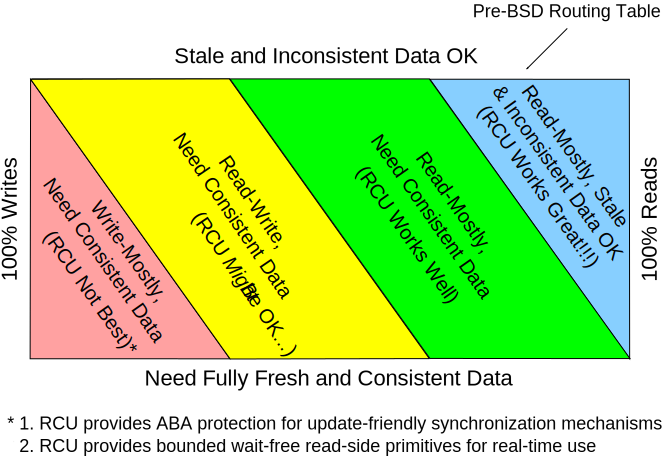
\includegraphics{defer/RCUApplicability}}
\caption{RCU Areas of Applicability}
\label{fig:defer:RCU Areas of Applicability}
\end{figure}

In the meantime,
\cref{fig:defer:RCU Areas of Applicability}
shows some rough rules of thumb on where RCU is most helpful.

As shown in the blue box at the top of the figure, RCU works best if
you have read-mostly data where stale and inconsistent
data is permissible (but see below for more information on stale and
inconsistent data).
The canonical example of this case in the Linux kernel is routing tables.
Because it may have taken many seconds or even minutes for the
routing updates to propagate across the Internet, the system
has been sending packets the wrong way for quite some time.
Having some small probability of continuing to send some of them the wrong
way for a few more milliseconds is almost never a problem.

If you have a read-mostly workload where consistent data is required,
RCU works well, as shown by the green ``read-mostly, need consistent data''
box.
One example of this case is the Linux kernel's mapping from user-level
System-V semaphore IDs to the corresponding in-kernel data structures.
Semaphores tend to be used far more frequently than they are created
and destroyed, so this mapping is read-mostly.
However, it would be erroneous to perform a semaphore operation on
a semaphore that has already been deleted.
This need for consistency is handled by using the lock in the
in-kernel semaphore data structure, along with a ``deleted''
flag that is set when deleting a semaphore.
If a user ID maps to an in-kernel data structure with the
``deleted'' flag set, the data structure is ignored, so that
the user ID is flagged as invalid.

Although this requires that the readers acquire a lock for the
data structure representing the semaphore itself,
it allows them to dispense with locking for the
mapping data structure.
The readers therefore locklessly
traverse the tree used to map from ID to data structure,
which in turn greatly improves performance, scalability, and
real-time response.

As indicated by the yellow ``read-write'' box, RCU can also be useful
for read-write
workloads where consistent data is required, although usually in
conjunction with a number of other synchronization primitives.
For example, the directory-entry cache in recent Linux kernels uses RCU in
conjunction with sequence locks, per-CPU locks, and per-data-structure
locks to allow lockless traversal of pathnames in the common case.
Although RCU can be very beneficial in this read-write case, such
use is often more complex than that of the read-mostly cases.

Finally, as indicated by the red box at the bottom of the figure,
update-mostly workloads requiring
consistent data are rarely good places to use RCU, though there are some
exceptions~\cite{MathieuDesnoyers2012URCU}.
In addition, as noted in
\cref{sec:defer:Type-Safe Memory},
within the Linux kernel, the \co{SLAB_TYPESAFE_BY_RCU}
slab-allocator flag provides type-safe memory to RCU readers, which can
greatly simplify \IXacrl{nbs} and other lockless
algorithms.

In short, RCU is an API that includes a publish-subscribe mechanism for
adding new data, a way of waiting for pre-existing RCU readers to finish,
and a discipline of maintaining multiple versions to allow updates to
avoid harming or unduly delaying concurrent RCU readers.
This RCU API is best suited for read-mostly situations, especially if
stale and inconsistent data can be tolerated by the application.

% defer/rcuAPI.tex

\subsection{RCU Linux-Kernel API}
\label{sec:defer:RCU Linux-Kernel API}
\OriginallyPublished{Section}{sec:defer:RCU Linux-Kernel API}{RCU Linux-Kernel API}{Linux Weekly News}{PaulEMcKenney2008WhatIsRCUAPI}

This section looks at RCU from the viewpoint of its Linux-kernel API.
Section~\ref{sec:defer:RCU has a Family of Wait-to-Finish APIs}
presents RCU's wait-to-finish APIs, and
Section~\ref{sec:defer:RCU has Publish-Subscribe and Version-Maintenance APIs}
presents RCU's publish-subscribe and version-maintenance APIs.
Finally,
Section~\ref{sec:defer:So, What is RCU Really?}
presents concluding remarks.

\subsubsection{RCU has a Family of Wait-to-Finish APIs}
\label{sec:defer:RCU has a Family of Wait-to-Finish APIs}

\begin{sidewaystable*}[htbp]
\centering
\footnotesize
\begin{tabularx}{7.9in}{>{\raggedright\arraybackslash}p{1.08in}|
    >{\raggedright\arraybackslash}X|
    >{\raggedright\arraybackslash}X|
    >{\raggedright\arraybackslash}X|
    >{\raggedright\arraybackslash}X|
    >{\raggedright\arraybackslash}p{1.22in}}
Attribute &
    RCU Classic &
	RCU BH &
	    RCU Sched &
		Realtime RCU &
		    SRCU \\
\hline
\hline
Purpose &
    Original &
	Prevent DDoS attacks &
	    Wait for preempt-disable regions, hardirqs, \& NMIs &
	        Realtime response &
		    Sleeping readers \\
\hline
Availability &
    2.5.43 &
	2.6.9 &
	    2.6.12 &
		2.6.26 &
		    2.6.19 \\
\hline
Read-side primitives &
    \tco{rcu_read_lock()}~! \tco{rcu_read_unlock()}~! &
	\tco{rcu_read_lock_bh()} \tco{rcu_read_unlock_bh()} &
	    \tco{preempt_disable()} \tco{preempt_enable()} (and friends) &
	        \tco{rcu_read_lock()} \tco{rcu_read_unlock()} &
		    \tco{srcu_read_lock()} \tco{srcu_read_unlock()} \\
\hline
{ Update-side primitives (synchronous) } &
    { \tco{synchronize_rcu()} \tco{synchronize_net()} } &
	\tco{synchronize_rcu_bh()} &
	    \tco{synchronize_sched()} &
	        { \tco{synchronize_rcu()} \tco{synchronize_net()} } &
		    \tco{synchronize_srcu()} \\
\hline
{ Update-side primitives (asynchronous/callback) } &
    \tco{call_rcu()} ! &
	\tco{call_rcu_bh()} &
	    \tco{call_rcu_sched()} &
	        \tco{call_rcu()} &
		    \tco{call_srcu()} \\
\hline
{ Update-side primitives (wait for callbacks) } &
    \tco{rcu_barrier()} &
	\tco{rcu_barrier_bh()} &
	    \tco{rcu_barrier_sched()} &
	        \tco{rcu_barrier()} &
		    N/A \\
\hline
Type-safe memory &
    \tco{SLAB_DESTROY_BY_RCU} &
	&
	    &
	        \tco{SLAB_DESTROY_BY_RCU} &
		    \\
\hline
Read side constraints &
    No blocking &
	No bottom-half (BH) enabling &
	    No blocking &
	        Only preemption and lock acquisition &
		    No \tco{synchronize_srcu()} with same \tco{srcu_struct} \\
\hline
Read side overhead &
    Preempt disable/enable (free on non-\tco{PREEMPT}) &
	BH disable/enable &
	    Preempt disable/enable (free on non-\tco{PREEMPT}) &
	        Simple instructions, \IRQ\ disable/enable &
		    Simple instructions, preempt disable/enable, memory barriers \\
\hline
Asynchronous update-side overhead &
    sub-microsecond &
	sub-microsecond &
	    sub-microsecond &
	        sub-microsecond &
		    N/A \\
\hline
Grace-period latency &
    10s of milliseconds &
	10s of milliseconds &
	    10s of milliseconds &
	        10s of milliseconds &
		    10s of milliseconds \\
\hline
Non-\tco{PREEMPT_RT} implementation &
    RCU Classic &
	RCU BH &
	    RCU Classic &
	        Preemptible RCU &
		    SRCU \\
\hline
\tco{PREEMPT_RT} implementation &
    Preemptible RCU &
	Realtime RCU &
	    Forced Schedule on all CPUs &
	        Realtime RCU &
		    SRCU \\
\end{tabularx}
\caption{RCU Wait-to-Finish APIs}
\label{tab:defer:RCU Wait-to-Finish APIs}
\end{sidewaystable*}

The most straightforward answer to ``what is RCU'' is that RCU is
an API used in the Linux kernel, as summarized by
Table~\ref{tab:defer:RCU Wait-to-Finish APIs},
which shows the wait-for-RCU-readers portions of the non-sleepable and
sleepable APIs, respectively,
and by
Table~\ref{tab:defer:RCU Publish-Subscribe and Version Maintenance APIs},
which shows the publish-subscribe portions of the API.

If you are new to RCU, you might consider focusing on just one
of the columns in
Table~\ref{tab:defer:RCU Wait-to-Finish APIs},
each of which summarizes one member of the Linux kernel's RCU API family.
For example, if you are primarily interested in understanding how RCU
is used in the Linux kernel, ``RCU Classic'' would be the place to start,
as it is used most frequently.
On the other hand, if you want to understand RCU for its own sake,
``SRCU'' has the simplest API.
You can always come back for the other columns later.

If you are already familiar with RCU, these tables can
serve as a useful reference.

\QuickQuiz{}
	Why do some of the cells in
	Table~\ref{tab:defer:RCU Wait-to-Finish APIs}
	have exclamation marks (``!'')?
\QuickQuizAnswer{
	The API members with exclamation marks (\co{rcu_read_lock()},
	\co{rcu_read_unlock()}, and \co{call_rcu()}) were the
	only members of the Linux RCU API that Paul E. McKenney was aware
	of back in the mid-90s.
	During this timeframe, he was under the mistaken impression that
	he knew all that there is to know about RCU.
} \QuickQuizEnd

The ``RCU Classic'' column corresponds to the original RCU implementation,
in which RCU read-side critical sections are delimited by
\co{rcu_read_lock()} and \co{rcu_read_unlock()}, which
may be nested.
The corresponding synchronous update-side primitives,
\co{synchronize_rcu()}, along with its synonym
\co{synchronize_net()}, wait for any currently executing
RCU read-side critical sections to complete.
The length of this wait is known as a ``grace period''.
The asynchronous update-side primitive, \co{call_rcu()},
invokes a specified function with a specified argument after a
subsequent grace period.
For example, \co{call_rcu(p,f);} will result in
the ``RCU callback'' \co{f(p)}
being invoked after a subsequent grace period.
There are situations,
such as when unloading a Linux-kernel module that uses \co{call_rcu()},
when it is necessary to wait for all
outstanding RCU callbacks to complete~\cite{PaulEMcKenney2007rcubarrier}.
The \co{rcu_barrier()} primitive does this job.
Note that the more recent hierarchical
RCU~\cite{PaulEMcKenney2008HierarchicalRCU}
implementation also adheres to ``RCU Classic'' semantics.

Finally, RCU may be used to provide
type-safe memory~\cite{Cheriton96a}, as described in
Section~\ref{sec:defer:RCU is a Way of Providing Type-Safe Memory}.
In the context of RCU, type-safe memory guarantees that a given
data element will not change type during any RCU read-side critical section
that accesses it.
To make use of RCU-based type-safe memory, pass
\co{SLAB_DESTROY_BY_RCU} to
\co{kmem_cache_create()}.
It is important to note that \co{SLAB_DESTROY_BY_RCU} will
\emph{in no way}
prevent \co{kmem_cache_alloc()} from immediately reallocating
memory that was just now freed via \co{kmem_cache_free()}!
In fact, the \co{SLAB_DESTROY_BY_RCU}-protected data structure
just returned by \co{rcu_dereference} might be freed and reallocated
an arbitrarily large number of times, even when under the protection
of \co{rcu_read_lock()}.
Instead, \co{SLAB_DESTROY_BY_RCU} operates by preventing
\co{kmem_cache_free()}
from returning a completely freed-up slab of data structures
to the system until after an RCU grace period elapses.
In short, although the data element might be freed and reallocated arbitrarily
often, at least its type will remain the same.

\QuickQuiz{}
	How do you prevent a huge number of RCU read-side critical
	sections from indefinitely blocking a \co{synchronize_rcu()}
	invocation?
\QuickQuizAnswer{
	There is no need to do anything to prevent RCU read-side
	critical sections from indefinitely blocking a
	\co{synchronize_rcu()} invocation, because the
	\co{synchronize_rcu()} invocation need wait only for
	\emph{pre-existing} RCU read-side critical sections.
	So as long as each RCU read-side critical section is
	of finite duration, there should be no problem.
} \QuickQuizEnd

\QuickQuiz{}
	The \co{synchronize_rcu()} API waits for all pre-existing
	interrupt handlers to complete, right?
\QuickQuizAnswer{
	Absolutely not!
	And especially not when using preemptible RCU!
	You instead want \co{synchronize_irq()}.
	Alternatively, you can place calls to \co{rcu_read_lock()}
	and \co{rcu_read_unlock()} in the specific interrupt handlers that
	you want \co{synchronize_rcu()} to wait for.
} \QuickQuizEnd

In the ``RCU BH'' column, \co{rcu_read_lock_bh()} and
\co{rcu_read_unlock_bh()} delimit RCU read-side critical
sections, \co{synchronize_rcu_bh()} waits for a grace period,
and \co{call_rcu_bh()} invokes the specified
function and argument after a later grace period.

\QuickQuiz{}
	What happens if you mix and match?
	For example, suppose you use \co{rcu_read_lock()} and
	\co{rcu_read_unlock()} to delimit RCU read-side critical
	sections, but then use \co{call_rcu_bh()} to post an
	RCU callback?
\QuickQuizAnswer{
	If there happened to be no RCU read-side critical
	sections delimited by \co{rcu_read_lock_bh()} and
	\co{rcu_read_unlock_bh()} at the time \co{call_rcu_bh()}
	was invoked, RCU would be within its rights to invoke the callback
	immediately, possibly freeing a data structure still being used by
	the RCU read-side critical section!
	This is not merely a theoretical possibility: a long-running RCU
	read-side critical section delimited by \co{rcu_read_lock()}
	and \co{rcu_read_unlock()} is vulnerable to this failure mode.

	However, the \co{rcu_dereference()} family of functions apply
	to all flavors of RCU.
	(There was an attempt to have per-flavor variants of
	\co{rcu_dereference()}, but it was just too messy.)
} \QuickQuizEnd

\QuickQuiz{}
	Hardware interrupt handlers can be thought of as being
	under the protection of an implicit \co{rcu_read_lock_bh()},
	right?
\QuickQuizAnswer{
	Absolutely not!
	And especially not when using preemptible RCU!
	If you need to access ``rcu\_bh''-protected data structures
	in an interrupt handler, you need to provide explicit calls to
	\co{rcu_read_lock_bh()} and \co{rcu_read_unlock_bh()}.
} \QuickQuizEnd

In the ``RCU Sched'' column, anything that disables preemption
acts as an RCU read-side critical section, and \co{synchronize_sched()}
waits for the corresponding RCU grace period.
This RCU API family was added in the 2.6.12 kernel, which split the
old \co{synchronize_kernel()} API into the current
\co{synchronize_rcu()} (for RCU Classic) and
\co{synchronize_sched()} (for RCU Sched).
Note that RCU Sched did not originally have an asynchronous
\co{call_rcu_sched()} interface, but one was added in 2.6.26.
In accordance with the quasi-minimalist philosophy of the Linux
community, APIs are added on an as-needed basis.

\QuickQuiz{}
	What happens if you mix and match RCU Classic and RCU Sched?
\QuickQuizAnswer{
	In a non-\co{PREEMPT} or a \co{PREEMPT} kernel, mixing these
	two works ``by accident'' because in those kernel builds, RCU Classic
	and RCU Sched map to the same implementation.
	However, this mixture is fatal in \co{PREEMPT_RT} builds using the -rt
	patchset, due to the fact that Realtime RCU's read-side critical
	sections can be preempted, which would permit
	\co{synchronize_sched()} to return before the
	RCU read-side critical section reached its \co{rcu_read_unlock()}
	call.
	This could in turn result in a data structure being freed before the
	read-side critical section was finished with it,
	which could in turn greatly increase the actuarial risk experienced
	by your kernel.

	In fact, the split between RCU Classic and RCU Sched was inspired
	by the need for preemptible RCU read-side critical sections.
} \QuickQuizEnd

\QuickQuiz{}
	In general, you cannot rely on \co{synchronize_sched()} to
	wait for all pre-existing interrupt handlers,
	right?
\QuickQuizAnswer{
	That is correct!
	Because -rt Linux uses threaded interrupt handlers, there can
	be context switches in the middle of an interrupt handler.
	Because \co{synchronize_sched()} waits only until each
	CPU has passed through a context switch, it can return
	before a given interrupt handler completes.

	If you need to wait for a given interrupt handler to complete,
	you should instead use \co{synchronize_irq()} or place
	explicit RCU read-side critical sections in the interrupt
	handlers that you wish to wait on.
} \QuickQuizEnd

The ``Realtime RCU'' column has the same API as does
RCU Classic, the only difference being that RCU read-side critical
sections may be preempted and may block while acquiring spinlocks.
The design of Realtime RCU is described
elsewhere~\cite{PaulEMcKenney2007PreemptibleRCU}.

The ``SRCU'' column in
Table~\ref{tab:defer:RCU Wait-to-Finish APIs}
displays a specialized RCU API that permits
general sleeping in RCU read-side critical
sections~\cite{PaulEMcKenney2006c}.
Of course,
use of \co{synchronize_srcu()} in an SRCU read-side
critical section can result in
self-deadlock, so should be avoided.
SRCU differs from earlier RCU implementations in that the caller
allocates an \co{srcu_struct} for each distinct SRCU
usage.
This approach prevents SRCU read-side critical sections from blocking
unrelated \co{synchronize_srcu()} invocations.
In addition, in this variant of RCU, \co{srcu_read_lock()}
returns a value that must be passed into the corresponding
\co{srcu_read_unlock()}.

\QuickQuiz{}
	Why should you be careful with \co{call_srcu()}?
\QuickQuizAnswer{
	A single task could register SRCU callbacks very quickly.
	Given that SRCU allows readers to block for arbitrary periods of
	time, this could consume an arbitrarily large quantity of memory.
	In contrast, given the synchronous \co{synchronize_srcu()}
	interface, a given task must finish waiting for a given grace period
	before it can start waiting for the next one.
} \QuickQuizEnd

\QuickQuiz{}
	Under what conditions can \co{synchronize_srcu()} be safely
	used within an SRCU read-side critical section?
\QuickQuizAnswer{
	In principle, you can use
	\co{synchronize_srcu()} with a given \co{srcu_struct}
	within an SRCU read-side critical section that uses some other
	\co{srcu_struct}.
	In practice, however, doing this is almost certainly a bad idea.
	In particular, the code shown in
	Listing~\ref{lst:defer:Multistage SRCU Deadlocks}
	could still result in deadlock.

\begin{listing}[htbp]
{
\begin{verbbox}
  1 idx = srcu_read_lock(&ssa);
  2 synchronize_srcu(&ssb);
  3 srcu_read_unlock(&ssa, idx);
  4
  5 /* . . . */
  6
  7 idx = srcu_read_lock(&ssb);
  8 synchronize_srcu(&ssa);
  9 srcu_read_unlock(&ssb, idx);
\end{verbbox}
}
\centering
\theverbbox
\caption{Multistage SRCU Deadlocks}
\label{lst:defer:Multistage SRCU Deadlocks}
\end{listing}
%
} \QuickQuizEnd

The Linux kernel currently has a surprising number of RCU APIs and
implementations.
There is some hope of reducing this number, evidenced by the fact
that a given build of the Linux kernel currently has at most
four implementations behind three APIs (given that RCU Classic
and Realtime RCU share the same API).
However, careful inspection and analysis will be required, just as
would be required in order to eliminate one of the many locking APIs.

The various RCU APIs are distinguished by the forward-progress
guarantees that their RCU read-side critical sections must provide,
and also by their scope, as follows:

\begin{enumerate}
\item	RCU BH: read-side critical sections
	must guarantee forward progress against everything except for
	NMI and interrupt handlers, but not including software-interrupt
	(\co{softirq}) handlers.
	RCU BH is global in scope.
\item	RCU Sched: read-side critical sections must guarantee forward
	progress against everything except for NMI and \IRQ\ handlers,
	including \co{softirq} handlers.
	RCU Sched is global in scope.
\item	RCU (both classic and real-time): read-side critical sections
	must guarantee forward progress against everything except for
	NMI handlers, \IRQ\ handlers, \co{softirq} handlers, and (in the
	real-time case) higher-priority real-time tasks.
	RCU is global in scope.
\item	SRCU: read-side critical sections need not guarantee
	forward progress unless some other task is waiting for the
	corresponding grace period to complete, in which case these
	read-side critical sections should complete in no more than
	a few seconds (and preferably much more quickly).\footnote{
		Thanks to James Bottomley for urging me to this
		formulation, as opposed to simply saying that
		there are no forward-progress guarantees.}
	SRCU's scope is defined by the use of the corresponding
	\co{srcu_struct}.
\end{enumerate}

In other words, SRCU compensate for their extremely weak
forward-progress guarantees by permitting the developer to restrict
their scope.

\subsubsection{RCU has Publish-Subscribe and Version-Maintenance APIs}
\label{sec:defer:RCU has Publish-Subscribe and Version-Maintenance APIs}

Fortunately, the RCU publish-subscribe and version-maintenance
primitives shown in the following
table apply to all of the variants of RCU discussed above.
This commonality can in some cases allow more code to be shared,
which certainly reduces the API proliferation that would otherwise
occur.
The original purpose of the RCU publish-subscribe APIs was to
bury memory barriers into these APIs, so that Linux kernel
programmers could use RCU without needing to become expert on
the memory-ordering models of each of the 20+ CPU families
that Linux supports~\cite{Spraul01}.

\begin{table*}[tb]
\renewcommand*{\arraystretch}{1.15}
\footnotesize
\centering
\begin{tabular}{lllp{1.2in}}
\toprule
Category &
	Primitives &
		Availability &
			Overhead \\
\midrule
List traversal &
	\tco{list_for_each_entry_rcu()} &
		2.5.59 &
			Simple instructions (memory barrier on Alpha) \\
\midrule
List update &
	\tco{list_add_rcu()} &
		2.5.44 &
			Memory barrier \\
&
	\tco{list_add_tail_rcu()} &
		2.5.44 &
			Memory barrier \\
&
	\tco{list_del_rcu()} &
		2.5.44 &
			Simple instructions \\
&
	\tco{list_replace_rcu()} &
		2.6.9 &
			Memory barrier \\
&
	\tco{list_splice_init_rcu()} &
		2.6.21 &
			Grace-period latency \\
\midrule
Hlist traversal &
	\tco{hlist_for_each_entry_rcu()} &
		2.6.8 &
			Simple instructions (memory barrier on Alpha) \\
&
	\tco{hlist_add_after_rcu()} &
		2.6.14 &
			Memory barrier \\
&
	\tco{hlist_add_before_rcu()} &
		2.6.14 &
			Memory barrier \\
&
	\tco{hlist_add_head_rcu()} &
		2.5.64 &
			Memory barrier \\
&
	\tco{hlist_del_rcu()} &
		2.5.64 &
			Simple instructions \\
&
	\tco{hlist_replace_rcu()} &
		2.6.15 &
			Memory barrier \\
\midrule
Pointer traversal &
	\tco{rcu_dereference()} &
		2.6.9 &
			Simple instructions (memory barrier on Alpha) \\
\midrule
Pointer update &
	\tco{rcu_assign_pointer()} &
		2.6.10 &
			Memory barrier \\
\bottomrule
\end{tabular}
\caption{RCU Publish-Subscribe and Version Maintenance APIs}
\label{tab:defer:RCU Publish-Subscribe and Version Maintenance APIs}
\end{table*}

The first pair of categories operate on Linux
\co{struct list_head} lists, which are circular, doubly-linked
lists.
The \co{list_for_each_entry_rcu()} primitive traverses an
RCU-protected list in a type-safe manner, while also enforcing
memory ordering for situations where a new list element is inserted
into the list concurrently with traversal.
On non-Alpha platforms, this primitive incurs little or no performance
penalty compared to \co{list_for_each_entry()}.
The \co{list_add_rcu()}, \co{list_add_tail_rcu()},
and \co{list_replace_rcu()} primitives are analogous to
their non-RCU counterparts, but incur the overhead of an additional
memory barrier on weakly-ordered machines.
The \co{list_del_rcu()} primitive is also analogous to its
non-RCU counterpart, but oddly enough is very slightly faster due to the
fact that it poisons only the \co{prev} pointer rather than
both the \co{prev} and \co{next} pointers as
\co{list_del()} must do.
Finally, the \co{list_splice_init_rcu()} primitive is similar
to its non-RCU counterpart, but incurs a full grace-period latency.
The purpose of this grace period is to allow RCU readers to finish
their traversal of the source list before completely disconnecting
it from the list header---failure to do this could prevent such
readers from ever terminating their traversal.

\QuickQuiz{}
	Why doesn't \co{list_del_rcu()} poison both the \co{next}
	and \co{prev} pointers?
\QuickQuizAnswer{
	Poisoning the \co{next} pointer would interfere
	with concurrent RCU readers, who must use this pointer.
	However, RCU readers are forbidden from using the \co{prev}
	pointer, so it may safely be poisoned.
} \QuickQuizEnd

The second pair of categories operate on Linux's
\co{struct hlist_head}, which is a linear linked list.
One advantage of \co{struct hlist_head} over
\co{struct list_head} is that the former requires only
a single-pointer list header, which can save significant memory in
large hash tables.
The \co{struct hlist_head} primitives in the table
relate to their non-RCU counterparts in much the same way as do the
\co{struct list_head} primitives.

The final pair of categories operate directly on pointers, and
are useful for creating RCU-protected non-list data structures,
such as RCU-protected arrays and trees.
The \co{rcu_assign_pointer()} primitive ensures that any
prior initialization remains ordered before the assignment to the
pointer on weakly ordered machines.
Similarly, the \co{rcu_dereference()} primitive ensures that subsequent
code dereferencing the pointer will see the effects of initialization code
prior to the corresponding \co{rcu_assign_pointer()} on
Alpha CPUs.
On non-Alpha CPUs, \co{rcu_dereference()} documents which pointer
dereferences are protected by RCU.

\QuickQuiz{}
	Normally, any pointer subject to \co{rcu_dereference()} \emph{must}
	always be updated using \co{rcu_assign_pointer()}.
	What is an exception to this rule?
\QuickQuizAnswer{
	One such exception is when a multi-element linked
	data structure is initialized as a unit while inaccessible to other
	CPUs, and then a single \co{rcu_assign_pointer()} is used
	to plant a global pointer to this data structure.
	The initialization-time pointer assignments need not use
	\co{rcu_assign_pointer()}, though any such assignments that
	happen after the structure is globally visible \emph{must} use
	\co{rcu_assign_pointer()}.

	However, unless this initialization code is on an impressively hot
	code-path, it is probably wise to use \co{rcu_assign_pointer()}
	anyway, even though it is in theory unnecessary.
	It is all too easy for a ``minor'' change to invalidate your cherished
	assumptions about the initialization happening privately.
} \QuickQuizEnd

\QuickQuiz{}
	Are there any downsides to the fact that these traversal and update
	primitives can be used with any of the RCU API family members?
\QuickQuizAnswer{
	It can sometimes be difficult for automated
	code checkers such as ``sparse'' (or indeed for human beings) to
	work out which type of RCU read-side critical section a given
	RCU traversal primitive corresponds to.
	For example, consider the code shown in
	Listing~\ref{lst:defer:Diverse RCU Read-Side Nesting}.

\begin{listing}[htbp]
{ \scriptsize
\begin{verbbox}
  1 rcu_read_lock();
  2 preempt_disable();
  3 p = rcu_dereference(global_pointer);
  4
  5 /* . . . */
  6
  7 preempt_enable();
  8 rcu_read_unlock();
\end{verbbox}
}
\centering
\theverbbox
\caption{Diverse RCU Read-Side Nesting}
\label{lst:defer:Diverse RCU Read-Side Nesting}
\end{listing}

	Is the \co{rcu_dereference()} primitive in an RCU Classic
	or an RCU Sched critical section?
	What would you have to do to figure this out?
} \QuickQuizEnd

\subsubsection{Where Can RCU's APIs Be Used?}
\label{sec:defer:Where Can RCU's APIs Be Used?}

\begin{figure}[tb]
\centering
\resizebox{3in}{!}{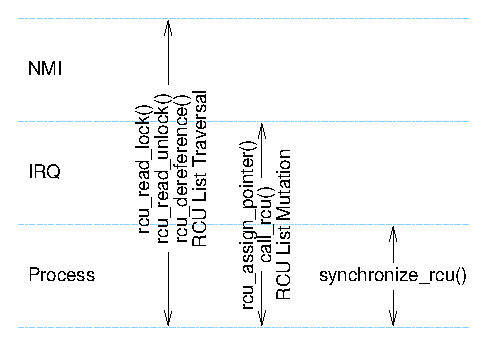
\includegraphics{defer/RCUenvAPI}}
\caption{RCU API Usage Constraints}
\label{fig:defer:RCU API Usage Constraints}
\end{figure}

Figure~\ref{fig:defer:RCU API Usage Constraints}
shows which APIs may be used in which in-kernel environments.
The RCU read-side primitives may be used in any environment, including NMI,
the RCU mutation and asynchronous grace-period primitives may be used in any
environment other than NMI, and, finally, the RCU synchronous grace-period
primitives may be used only in process context.
The RCU list-traversal primitives include \co{list_for_each_entry_rcu()},
\co{hlist_for_each_entry_rcu()}, etc.
Similarly, the RCU list-mutation primitives include
\co{list_add_rcu()}, \co{hlist_del_rcu()}, etc.

Note that primitives from other families of RCU may be substituted,
for example, \co{srcu_read_lock()} may be used in any context
in which \co{rcu_read_lock()} may be used.

\subsubsection{So, What \emph{is} RCU Really?}
\label{sec:defer:So, What is RCU Really?}

At its core, RCU is nothing more nor less than an API that supports
publication and subscription for insertions, waiting for all RCU readers
to complete, and maintenance of multiple versions.
That said, it is possible to build higher-level constructs
on top of RCU, including the reader-writer-locking, reference-counting,
and existence-guarantee constructs listed in
Section~\ref{sec:defer:RCU Usage}.
Furthermore, I have no doubt that the Linux community will continue to
find interesting new uses for RCU,
just as they do for any of a number of synchronization
primitives throughout the kernel.

Of course, a more-complete view of RCU would also include
all of the things you can do with these APIs.

However, for many people, a complete view of RCU must include sample
RCU implementations.
The next section therefore presents a series of ``toy'' RCU implementations
of increasing complexity and capability.

% defer/toyrcu.tex

\section{``Toy'' RCU Implementations}
\label{defer:``Toy'' RCU Implementations}

The toy RCU implementations in this section are designed not for
high performance, practicality, or any kind of production use,
but rather for clarity.
Nevertheless, you will need a thorough understanding of
Chapters~\ref{chp:Introduction} and
\ref{chp:defer:Deferred Processing}
for even these toy RCU implementations to be easily understandable.

Section~\ref{defer:Lock-Based RCU} presents a rudimentary
RCU implementation based on simple locking, while
Section~\ref{defer:Simple Counter-Based RCU} through
\ref{defer:Scalable Counter-Based RCU With Shared Grace Periods}
present a series of
simple RCU implementations based on locking, reference counters,
and free-running counters.

\subsection{Lock-Based RCU}
\label{defer:Lock-Based RCU}

\begin{figure}[bp]
{ \scriptsize
\begin{verbatim}
  1 static void rcu_read_lock(void)
  2 {
  3   spin_lock(&rcu_gp_lock);
  4 }
  5 
  6 static void rcu_read_unlock(void)
  7 {
  8   spin_unlock(&rcu_gp_lock);
  9 }
 10 
 11 void synchronize_rcu(void)
 12 {
 13   spin_lock(&rcu_gp_lock);
 14   spin_unlock(&rcu_gp_lock);
 15 }
\end{verbatim}
}
\caption{Lock-Based RCU Implementation}
\label{fig:defer:Lock-Based RCU Implementation}
\end{figure}

Perhaps the simplest RCU implementation leverages locking, as
shown in
Figure~\ref{fig:defer:Lock-Based RCU Implementation}
(\url{rcu_lock.h} and \url{rcu_lock.c}).
In this implementation, \url{rcu_read_lock()} acquires a global
spinlock, \url{rcu_read_unlock()} releases it, and
\url{synchronize_rcu()} acquires it then immediately releases it.

Because \url{synchronize_rcu()} does not return until it has acquired
(and released) the lock, it cannot return until all prior RCU read-side
critical sections have completed, thus faithfully implementing
RCU semantics.
Of course, only one RCU reader may be in its read-side critical section
at a time, which almost entirely defeats the purpose of RCU.
In addition, the lock operations in \url{rcu_read_lock()} and
\url{rcu_read_unlock()} are extremely heavyweight,
with read-side overhead ranging from about 100~nanoseconds on a single Power5
CPU up to almost 18~\emph{microseconds} on a 64-CPU system.
Worse yet,
these same lock operations permit \url{rcu_read_lock()}
to participate in deadlock cycles.
Furthermore, in absence of recursive locks, 
RCU read-side critical sections cannot be nested, and, finally,
although concurrent RCU updates could in principle be satisfied by
a common grace period, this implementation serializes grace periods,
preventing grace-period sharing.

\QuickQuiz{Why wouldn't any deadlock in the RCU implementation in
	Figure~\ref{fig:defer:Lock-Based RCU Implementation}
	also be a deadlock in any other RCU implementation?}
\QuickQuizAnswer{

\begin{figure}[tbp]
{ \scriptsize
\begin{verbatim}
  1 void foo(void)
  2 {
  3   spin_lock(&my_lock);
  4   rcu_read_lock();
  5   do_something();
  6   rcu_read_unlock();
  7   do_something_else();
  8   spin_unlock(&my_lock);
  9 }
 10 
 11 void bar(void)
 12 {
 13   rcu_read_lock();
 14   spin_lock(&my_lock);
 15   do_some_other_thing();
 16   spin_unlock(&my_lock);
 17   do_whatever();
 18   rcu_read_unlock();
 19 }
\end{verbatim}
}
\caption{Deadlock in Lock-Based RCU Implementation}
\label{fig:defer:Deadlock in Lock-Based RCU Implementation}
\end{figure}

	Suppose the functions \url{foo()} and \url{bar()} in
	Figure~\ref{fig:defer:Deadlock in Lock-Based RCU Implementation}
	are invoked concurrently from different CPUs.
	Then \url{foo()} will acquire \url{my_lock()} on line~3,
	while \url{bar()} will acquire \url{rcu_gp_lock} on
	line~13.
	When \url{foo()} advances to line~4, it will attempt to
	acquire \url{rcu_gp_lock}, which is held by \url{bar()}.
	Then when \url{bar()} advances to line~14, it will attempt
	to acquire \url{my_lock}, which is held by \url{foo()}.

	Each function is then waiting for a lock that the other
	holds, a classic deadlock.

	Other RCU implementations neither spin nor block in
	\url{rcu_read_lock()}, hence avoiding deadlocks.
} \QuickQuizEnd

\QuickQuiz{Why not simply use reader-writer locks in the RCU implementation
	in
	Figure~\ref{fig:defer:Lock-Based RCU Implementation}
	in order to allow RCU readers to proceed in parallel?}
\QuickQuizAnswer{
	One could in fact use reader-writer locks in this manner.
	However, textbook reader-writer locks suffer from memory
	contention, so that the RCU read-side critical sections would
	need to be quite long to actually permit parallel execution.
	@@@ add reference to reader-writer locking discussion from LJ2003 @@@

	On the other hand, use of a reader-writer lock that is
	read-acquired in \url{rcu_read_lock()} would avoid the
	deadlock condition noted above.
} \QuickQuizEnd

It is hard to imagine this implementation being useful
in a production setting, though it does have the virtue
of being implementable in almost any user-level application.
Furthermore, similar implementations having one lock per CPU
or using reader-writer locks actually have been used in production
in the 2.4 Linux kernel.

The counter-based RCU implementation described next overcomes some of
the shortcomings of the lock-based implementation.

\subsection{Simple Counter-Based RCU}
\label{defer:Simple Counter-Based RCU}

\begin{figure}[tbp]
{ \scriptsize
\begin{verbatim}
  1 atomic_t rcu_refcnt;
  2 
  3 static void rcu_read_lock(void)
  4 {
  5   atomic_inc(&rcu_refcnt);
  6   smp_mb();
  7 }
  8 
  9 static void rcu_read_unlock(void)
 10 {
 11   smp_mb();
 12   atomic_dec(&rcu_refcnt);
 13 }
 14 
 15 void synchronize_rcu(void)
 16 {
 17   smp_mb();
 18   while (atomic_read(&rcu_refcnt) != 0) {
 19     poll(NULL, 0, 10);
 20   }
 21   smp_mb();
 22 }
\end{verbatim}
}
\caption{RCU Implementation Using Single Global Reference Counter}
\label{fig:defer:RCU Implementation Using Single Global Reference Counter}
\end{figure}

A slightly more sophisticated RCU implementation is shown in
Figure~\ref{fig:defer:RCU Implementation Using Single Global Reference Counter}
(\url{rcu_rcg.h} and \url{rcu_rcg.c}).
This implementation makes use of a global reference counter
\url{rcu_refcnt} defined on line~1.
The \url{rcu_read_lock()} primitive atomically increments this
counter, then executes a memory barrier to ensure that the
RCU read-side critical section is ordered after the atomic
increment.
Similarly, \url{rcu_read_unlock()} executes a memory barrier to
confine the RCU read-side critical section, then atomically
decrements the counter.
The \url{synchronize_rcu()} primitive spins waiting for the reference
counter to reach zero, surrounded by memory barriers.
The \url{poll()} on line~19 merely provides pure delay, and from
a pure RCU-semantics point of view could be omitted.
Again, once \url{synchronize_rcu()} returns, all prior
RCU read-side critical sections are guaranteed to have completed.

In happy contrast to the lock-based implementation shown in
Appendix~\ref{defer:Lock-Based RCU}, this implementation
allows parallel execution of RCU read-side critical sections,
and also allows them to be nested.
In addition, the \url{rcu_read_lock()} primitive cannot possibly
participate in deadlock cycles, as it never spins nor blocks.

However, this implementations still has some serious shortcomings.
First, the atomic operations in \url{rcu_read_lock()} and
\url{rcu_read_unlock()} are still quite  heavyweight,
with read-side overhead ranging from about 100~nanoseconds on
a single Power5 CPU up to more than 20~\emph{microseconds}
on a 64-CPU system.
This means that the RCU read-side critical sections
have to be extremely long in order to get any real
read-side parallelism.
On the other hand, in the absence of readers, grace periods elapse
in about 40~\emph{nanoseconds}, many orders of magnitude faster
than production-quality implementations in the Linux kernel.
Second, if there are many concurrent \url{rcu_read_lock()}
and \url{rcu_read_unlock()} operations, there will
be extreme memory contention on \url{rcu_refcnt},
resulting in expensive cache misses.
Both of these first two shortcomings largely defeat a major purpose of
RCU, namely to provide low-overhead read-side synchronization primitives.
Third, a large number of RCU readers with long read-side
critical sections could prevent \url{synchronize_rcu()}
from ever completing, as the global counter might
never reach zero.
This could result in starvation of RCU updates, which
is of course unacceptable in production settings.
Finally, although concurrent RCU updates could in principle be
satisfied by a common grace period, this implementation
serializes grace periods, preventing grace-period
sharing.

\QuickQuiz{Why not simply make \url{rcu_read_lock()} wait when a concurrent
	\url{synchronize_rcu()} has been waiting too long in
	the RCU implementation in
	Figure~\ref{fig:defer:RCU Implementation Using Single Global Reference Counter}?
	Wouldn't that prevent \url{synchronize_rcu()} from starving?}
\QuickQuizAnswer{
	Although this would in fact eliminate the starvation, it would
	also mean that \url{rcu_read_lock()} would spin or block waiting
	for the writer, which is in turn waiting on readers.
	If one of these readers is attempting to acquire a lock that
	the spinning/blocking \url{rcu_read_lock()} holds, we again
	have deadlock.

	In short, the cure is worse than the disease.
	See Section~\ref{defer:Starvation-Free Counter-Based RCU}
	for a proper cure.
} \QuickQuizEnd

Therefore, it is still hard to imagine this implementation being useful
in a production setting, though it has a bit more potential
than the lock-based mechanism, for example, as an RCU implementation
suitable for a high-stress debugging environment.
The next section describes a variation on the reference-counting
scheme that is more favorable to writers.

\subsection{Starvation-Free Counter-Based RCU}
\label{defer:Starvation-Free Counter-Based RCU}

\begin{figure}[tbp]
{ \scriptsize
\begin{verbatim}
  1 static void rcu_read_lock(void)
  2 {
  3   int i;
  4   int n;
  5 
  6   n = __get_thread_var(rcu_nesting);
  7   if (n == 0) {
  8     i = atomic_read(&rcu_idx);
  9     __get_thread_var(rcu_read_idx) = i;
 10     atomic_inc(&rcu_refcnt[i]);
 11   }
 12   __get_thread_var(rcu_nesting) = n + 1;
 13   smp_mb();
 14 }
 15 
 16 static void rcu_read_unlock(void)
 17 {
 18   int i;
 19   int n;
 20 
 21   smp_mb();
 22   n = __get_thread_var(rcu_nesting);
 23   if (n == 1) {
 24      i = __get_thread_var(rcu_read_idx);
 25     atomic_dec(&rcu_refcnt[i]);
 26   }
 27   __get_thread_var(rcu_nesting) = n - 1;
 28 }
\end{verbatim}
}
\caption{RCU Read-Side Using Global Reference-Count Pair}
\label{fig:defer:RCU Read-Side Using Global Reference-Count Pair}
\end{figure}

Figure~\ref{fig:defer:RCU Read-Side Using Global Reference-Count Pair}
(\url{rcu_rcgp.h})
shows the read-side primitives of an RCU implementation that uses a pair
of reference counters (\url{rcu_refcnt[]}),
along with a global index that
selects one counter out of the pair (\url{rcu_idx}),
a per-thread nesting counter \url{rcu_nesting},
a per-thread snapshot of the global index (\url{rcu_read_idx}),
and a global lock (\url{rcu_gp_lock}).

The \url{rcu_read_lock()} primitive atomically increments the member of the
\url{rcu_refcnt[]} pair indexed by \url{rcu_idx}, and keeps a
snapshot of this index in the per-thread variable \url{rcu_read_idx}.
The \url{rcu_read_unlock()} primitive then atomically decrements
whichever counter of the pair that the corresponding \url{rcu_read_lock()}
incremented.
However, because only one value of \url{rcu_idx} is remembered per thread,
additional measures must be taken to permit nesting.
These additional measures use the per-thread \url{rcu_nesting} variable
to track nesting.

To make all this work, line~6 of \url{rcu_read_lock()} in
Figure~\ref{fig:defer:RCU Read-Side Using Global Reference-Count Pair}
picks up the
current thread's instance of \url{rcu_nesting}, and if line~7 finds
that this is the outermost \url{rcu_read_lock()},
then lines~8-10 pick up the current value of
\url{rcu_idx}, save it in this thread's instance of \url{rcu_read_idx},
and atomically increment the selected element of \url{rcu_refcnt}.
Regardless of the value of \url{rcu_nesting}, line~12 increments it.
Line~13 executes a memory barrier to ensure that the RCU read-side
critical section does not bleed out before the \url{rcu_read_lock()} code.

Similarly, the \url{rcu_read_unlock()} function executes a memory barrier
at line~21
to ensure that the RCU read-side critical section does not bleed out
after the \url{rcu_read_unlock()} code.
Line~22 picks up this thread's instance of \url{rcu_nesting}, and if
line~23 finds that this is the outermost \url{rcu_read_unlock()},
then lines~24 and 25 pick up this thread's instance of \url{rcu_read_idx}
(saved by the outermost \url{rcu_read_lock()}) and atomically decrements
the selected element of \url{rcu_refcnt}.
Regardless of the nesting level, line~27 decrements this thread's
instance of \url{rcu_nesting}.

\begin{figure}[tbp]
{ \scriptsize
\begin{verbatim}
  1 void synchronize_rcu(void)
  2 {
  3   int i;
  4 
  5   smp_mb();
  6   spin_lock(&rcu_gp_lock);
  7   i = atomic_read(&rcu_idx);
  8   atomic_set(&rcu_idx, !i);
  9   smp_mb();
 10   while (atomic_read(&rcu_refcnt[i]) != 0) {
 11     poll(NULL, 0, 10);
 12   }
 13   smp_mb();
 14   atomic_set(&rcu_idx, i);
 15   smp_mb();
 16   while (atomic_read(&rcu_refcnt[!i]) != 0) {
 17     poll(NULL, 0, 10);
 18   }
 19   spin_unlock(&rcu_gp_lock);
 20   smp_mb();
 21 }
\end{verbatim}
}
\caption{RCU Update Using Global Reference-Count Pair}
\label{fig:defer:RCU Update Using Global Reference-Count Pair}
\end{figure}

Figure~\ref{fig:defer:RCU Update Using Global Reference-Count Pair}
(\url{rcu_rcpg.c})
shows the corresponding \url{synchronize_rcu()} implementation.
Lines~6 and 19 acquire and release \url{rcu_gp_lock} in order to
prevent more than one concurrent instance of \url{synchronize_rcu()}.
Lines~7-8 pick up the value of \url{rcu_idx} and complement it,
respectively, so that subsequent instances of \url{rcu_read_lock()}
will use a different element of \url{rcu_idx} that did preceding
instances.
Lines~10-12 then wait for the prior element of \url{rcu_idx} to
reach zero, with the memory barrier on line~9 ensuring that the check
of \url{rcu_idx} is not reordered to precede the complementing of
\url{rcu_idx}.
Lines~13-18 repeat this process, and line~20 ensures that any
subsequent reclamation operations are not reordered to precede the
checking of \url{rcu_refcnt}.

\QuickQuiz{Why the memory barrier on line~5 of \url{synchronize_rcu()} in
	Figure~\ref{fig:defer:RCU Update Using Global Reference-Count Pair}
	given that there is a spin-lock acquisition immediately after?}
\QuickQuizAnswer{
	The spin-lock acquisition only guarantees that the spin-lock's
	critical section will not ``bleed out'' to precede the
	acquisition.
	It in no way guarantees that code preceding the spin-lock
	acquisitoin won't be reordered into the critical section.
	Such reordering could cause a removal from an RCU-protected
	list to be reordered to follow the complementing of
	\url{rcu_idx}, which could allow a newly starting RCU
	read-side critical section to see the recently removed
	data element.

	Exercise for the reader: use a tool such as Promela/spin
	to determine which (if any) of the memory barriers in
	Figure~\ref{fig:defer:RCU Update Using Global Reference-Count Pair}
	are really needed.
	See Section~\ref{app:formal:Formal Verification}
	for information on using these tools.
	The first correct and complete response will be credited.
} \QuickQuizEnd

\QuickQuiz{Why is the counter flipped twice in
	Figure~\ref{fig:defer:RCU Update Using Global Reference-Count Pair}?
	Shouldn't a single flip-and-wait cycle be sufficient?}
\QuickQuizAnswer{
	Both flips are absolutely required.
	To see this, consider the following sequence of events:
	\begin{enumerate}
	\item	Line~8 of \url{rcu_read_lock()} in
		Figure~\ref{fig:defer:RCU Read-Side Using Global Reference-Count Pair}
		picks up \url{rcu_idx}, finding its value to be zero.
	\item	Line~8 of \url{synchronize_rcu()} in
		Figure~\ref{fig:defer:RCU Update Using Global Reference-Count Pair}
		complements the value of \url{rcu_idx}, setting its
		value to one.
	\item	Lines~10-13 of \url{synchronize_rcu()} find that the
		value of \url{rcu_refcnt[0]} is zero, and thus
		returns.
		(Recall that the question is asking what happens if
		lines~14-20 are omitted.)
	\item	Lines~9 and 10 of \url{rcu_read_lock()} store the
		value zero to this thread's instance of \url{rcu_read_idx}
		and increments \url{rcu_refcnt[0]}, respectively.
		Execution then proceeds into the RCU read-side critical
		section.
		\label{defer:rcu_rcgp:RCU Read Side Start}
	\item	Another instance of \url{synchronize_rcu()} again complements
		\url{rcu_idx}, this time setting its value to zero.
		Because \url{rcu_refcnt[1]} is zero, \url{synchronize_rcu()}
		returns immediately.
		(Recall that \url{rcu_read_lock()} incremented
		\url{rcu_refcnt[0]}, not \url{rcu_refcnt[1]}!)
		\label{defer:rcu_rcgp:RCU Grace Period Start}
	\item	The grace period that started in
		step~\ref{defer:rcu_rcgp:RCU Grace Period Start}
		has been allowed to end, despite
		the fact that the RCU read-side critical section
		that started beforehand in
		step~\ref{defer:rcu_rcgp:RCU Read Side Start}
		has not completed.
		This violates RCU semantics, and could allow the update
		to free a data element that the RCU read-side critical
		section was still referencing.
	\end{enumerate}

	Exercise for the reader: What happens if \url{rcu_read_lock()}
	is preempted for a very long time (hours!) just after
	line~8?
	Does this implementation operate correctly in that case?
	Why or why not?
	The first correct and complete response will be credited.
} \QuickQuizEnd

This implementation avoids the update-starvation issues that could
occur in the single-counter implementation shown in
Figure~\ref{fig:defer:RCU Implementation Using Single Global Reference Counter}.

There are still some serious shortcomings.
First, the atomic operations in \url{rcu_read_lock()}
and \url{rcu_read_unlock()}
are still quite heavyweight.
In fact, they are more complex than those
of the single-counter variant shown in
Figure~\ref{fig:defer:RCU Implementation Using Single Global Reference Counter},
with the read-side primitives consuming about 150~nanoseconds on a single
Power5 CPU and almost 40~\emph{microseconds} on a 64-CPU system.
The updates-side \url{synchronize_rcu()} primitive is more costly as
well, ranging from about 200~nanoseconds on a single Power5 CPU to
more than 40~\emph{microseconds} on a 64-CPU system.
This means that the RCU read-side critical sections
have to be extremely long in order to get any real
read-side parallelism.
Second, if there are many concurrent \url{rcu_read_lock()}
and \url{rcu_read_unlock()} operations, there will
be extreme memory contention on the \url{rcu_refcnt}
elements, resulting in expensive cache misses.
This further extends the RCU read-side critical-section
duration required to provide parallel read-side access.
These first two shortcomings defeat the purpose of RCU in most
situations.
Third, the need to flip \url{rcu_idx} twice imposes substantial
overhead on updates, especially if there are large
numbers of threads.
Finally, despite the fact that concurrent RCU updates could in principle be
satisfied by a common grace period, this implementation
serializes grace periods, preventing grace-period
sharing.

\QuickQuiz{Given that atomic increment and decrement are so expensive,
	why not just use non-atomic increment on line~10 and a
	non-atomic decrement on line~25 of
	Figure~\ref{fig:defer:RCU Read-Side Using Global Reference-Count Pair}?}
\QuickQuizAnswer{
	Using non-atomic operations would cause increments and decrements
	to be lost, in turn causing the implementation to fail.
	See Section~\ref{defer:Scalable Counter-Based RCU}
	for a safe way to use non-atomic operations in
	\url{rcu_read_lock()} and \url{rcu_read_unlock()}.
} \QuickQuizEnd

Despite these shortcomings, one could imagine this variant
of RCU being used on small tightly coupled multiprocessors,
perhaps as a memory-conserving implementation that maintains
API compatibility with more complex implementations.
However, it would not not likely scale well beyond a few CPUs.

The next section describes yet another variation on the reference-counting
scheme that provides greatly improved read-side performance and scalability.

\subsection{Scalable Counter-Based RCU}
\label{defer:Scalable Counter-Based RCU}

\begin{figure}[tbp]
{ \scriptsize
\begin{verbatim}
  1 static void rcu_read_lock(void)
  2 {
  3   int i;
  4   int n;
  5 
  6   n = __get_thread_var(rcu_nesting);
  7   if (n == 0) {
  8     i = atomic_read(&rcu_idx);
  9     __get_thread_var(rcu_read_idx) = i;
 10     __get_thread_var(rcu_refcnt)[i]++;
 11   }
 12   __get_thread_var(rcu_nesting) = n + 1;
 13   smp_mb();
 14 }
 15 
 16 static void rcu_read_unlock(void)
 17 {
 18   int i;
 19   int n;
 20 
 21   smp_mb();
 22   n = __get_thread_var(rcu_nesting);
 23   if (n == 1) {
 24      i = __get_thread_var(rcu_read_idx);
 25     __get_thread_var(rcu_refcnt)[i]--;
 26   }
 27   __get_thread_var(rcu_nesting) = n - 1;
 28 }
\end{verbatim}
}
\caption{RCU Read-Side Using Per-Thread Reference-Count Pair}
\label{fig:defer:RCU Read-Side Using Per-Thread Reference-Count Pair}
\end{figure}

Figure~\ref{fig:defer:RCU Read-Side Using Per-Thread Reference-Count Pair}
(\url{rcu_rcpl.h})
shows the read-side primitives of an RCU implementation that uses per-thread
pairs of reference counters.
This implementation is quite similar to that shown in
Figure~\ref{fig:defer:RCU Read-Side Using Global Reference-Count Pair},
the only difference being that \url{rcu_refcnt} is now a per-thread
variable, so the \url{rcu_read_lock()} and
\url{rcu_read_unlock()} primitives no longer perform atomic operations.

\QuickQuiz{Come off it!
	We can see the \url{atomic_read()} primitive in
	\url{rcu_read_lock()}!!!
	So why are you trying to pretend that \url{rcu_read_lock()}
	contains no atomic operations???}
\QuickQuizAnswer{
	The \url{atomic_read()} primitives does not actually execute
	atomic machine instructions, but rather does a normal load
	from an \url{atomic_t}.
} \QuickQuizEnd

\begin{figure}[tbp]
{ \scriptsize
\begin{verbatim}
  1 static void flip_counter_and_wait(int i)
  2 {
  3   int t;
  4 
  5   atomic_set(&rcu_idx, !i);
  6   smp_mb();
  7   for_each_thread(t) {
  8     while (per_thread(rcu_refcnt, t)[i] != 0) {
  9       poll(NULL, 0, 10);
 10     }
 11   }
 12   smp_mb();
 13 }
 14 
 15 void synchronize_rcu(void)
 16 {
 17   int i;
 18 
 19   smp_mb();
 20   spin_lock(&rcu_gp_lock);
 21   i = atomic_read(&rcu_idx);
 22   flip_counter_and_wait(i);
 23   flip_counter_and_wait(!i);
 24   spin_unlock(&rcu_gp_lock);
 25   smp_mb();
 26 }
\end{verbatim}
}
\caption{RCU Update Using Per-Thread Reference-Count Pair}
\label{fig:defer:RCU Update Using Per-Thread Reference-Count Pair}
\end{figure}

Figure~\ref{fig:defer:RCU Update Using Per-Thread Reference-Count Pair}
(\url{rcu_rcpl.c})
shows the implementation of \url{synchronize_rcu()}, along with a helper
function named \url{flip_counter_and_wait()}.
The \url{synchronize_rcu()} function resembles that shown in
Figure~\ref{fig:defer:RCU Update Using Global Reference-Count Pair},
except that the repeated counter flip is replaced by a pair of calls
on lines~22 and 23 to the new helper function.

The new \url{flip_counter_and_wait()} function updates the
\url{rcu_idx} variable on line~5, executes a memory barrier on line~6,
then lines~7-11 spin on each thread's prior \url{rcu_refcnt} element,
waiting for it to go to zero.
Once all such elements have gone to zero,
it executes another memory barrier on line~12 and returns.

This RCU implementation imposes important new requirements on its
software environment, namely, (1) that it be possible to declare
per-thread variables, (2) that these per-thread variables be accessible
from other threads, and (3) that it is possible to enumerate all threads.
These requirements can be met in almost all software environments,
but often result in fixed upper bounds on the number of threads.
More-complex implementations might avoid such bounds, for example, by using
expandable hash tables.
Such implementations might dynamically track threads, for example, by
adding them on their first call to \url{rcu_read_lock()}.

\QuickQuiz{Great, if we have $N$ threads, we can have $2N$ ten-millisecond
	waits (one set per \url{flip_counter_and_wait()} invocation,
	and even that assumes that we wait only once for each thread.
	Don't we need the grace period to complete \emph{much} more quickly?}
\QuickQuizAnswer{
	Keep in mind that we only wait for a given thread if that thread
	is still in a pre-existing RCU read-side critical section,
	and that waiting for one hold-out thread gives all the other
	threads a chance to complete any pre-existing RCU read-side
	critical sections that they might still be executing.
	So the only way that we would wait for $2N$ intervals
	would be if the last thread still remained in a pre-existing
	RCU read-side critical section despite all the waiting for
	all the prior threads.
	In short, this implementation will not wait unnecessarily.

	However, if you are stress-testing code that uses RCU, you
	might want to comment out the \url{poll()} statement in
	order to better catch bugs that incorrectly retain a reference
	to an RCU-protected data element outside of an RCU
	read-side critical section.
} \QuickQuizEnd

This implementation still has several shortcomings.
First, the need to flip \url{rcu_idx} twice imposes substantial overhead
on updates, especially if there are large numbers of threads.
Second, \url{synchronize_rcu()} must now examine a number of variables
that increases linearly with the number of threads, imposing substantial
overhead on applications with large numbers of threads.
Third, as before, although concurrent RCU updates could in principle
be satisfied by a common grace period, this implementation serializes
grace periods, preventing grace-period sharing.
Finally, as noted in the text, the need for per-thread variables
and for enumerating threads may be problematic in some software
environments.

That said, the read-side primitives scale very nicely, requiring about
115~nanoseconds regardless of whether running on a single-CPU or a 64-CPU
Power5 system.
As noted above, the \url{synchronize_rcu()} primitive does not scale,
ranging in overhead from about a microsecond on a single Power5 CPU
up to almost 200~microseconds on a 64-CPU system.
this implementation could conceivably form the basis for a
production-quality user-level RCU implementation.

The next section describes an algorithm permitting more efficient
concurrent RCU updates.

\subsection{Scalable Counter-Based RCU With Shared Grace Periods}
\label{defer:Scalable Counter-Based RCU With Shared Grace Periods}

\begin{figure}[tbp]
{ \scriptsize
\begin{verbatim}
  1 static void rcu_read_lock(void)
  2 {
  3   int i;
  4   int n;
  5 
  6   n = __get_thread_var(rcu_nesting);
  7   if (n == 0) {
  8     i = ACCESS_ONCE(rcu_idx) & 0x1;
  9     __get_thread_var(rcu_read_idx) = i;
 10     __get_thread_var(rcu_refcnt)[i]++;
 11   }
 12   __get_thread_var(rcu_nesting) = n + 1;
 13   smp_mb();
 14 }
 15 
 16 static void rcu_read_unlock(void)
 17 {
 18   int i;
 19   int n;
 20 
 21   smp_mb();
 22   n = __get_thread_var(rcu_nesting);
 23   if (n == 1) {
 24      i = __get_thread_var(rcu_read_idx);
 25     __get_thread_var(rcu_refcnt)[i]--;
 26   }
 27   __get_thread_var(rcu_nesting) = n - 1;
 28 }
\end{verbatim}
}
\caption{RCU Read-Side Using Per-Thread Reference-Count Pair and Shared Update}
\label{fig:defer:RCU Read-Side Using Per-Thread Reference-Count Pair and Shared Update}
\end{figure}

Figure~\ref{fig:defer:RCU Read-Side Using Per-Thread Reference-Count Pair and Shared Update}
(\url{rcu_rcpls.h})
shows the read-side primitives for an RCU implementation using per-thread
reference count pairs, as before, but permitting updates to share
grace periods.
The main difference from the earlier implementation shown in
Figure~\ref{fig:defer:RCU Read-Side Using Per-Thread Reference-Count Pair}
is that \url{rcu_idx} is now a \url{long} that counts freely,
so that line~8 of
Figure~\ref{fig:defer:RCU Read-Side Using Per-Thread Reference-Count Pair and Shared Update}
must mask off the low-order bit.
We also switched from using \url{atomic_read()} and \url{atomic_set()}
to using \url{ACCESS_ONCE()}.

\begin{figure}[tbp]
{ \scriptsize
\begin{verbatim}
  1 static void flip_counter_and_wait(int ctr)
  2 {
  3   int i;
  4   int t;
  5 
  6   ACCESS_ONCE(rcu_idx) = ctr + 1;
  7   i = ctr & 0x1;
  8   smp_mb();
  9   for_each_thread(t) {
 10     while (per_thread(rcu_refcnt, t)[i] != 0) {
 11       poll(NULL, 0, 10);
 12     }
 13   }
 14   smp_mb();
 15 }
 16 
 17 void synchronize_rcu(void)
 18 {
 19   int ctr;
 20   int oldctr;
 21 
 22   smp_mb();
 23   oldctr = ACCESS_ONCE(rcu_idx);
 24   smp_mb();
 25   spin_lock(&rcu_gp_lock);
 26   ctr = ACCESS_ONCE(rcu_idx);
 27   if (ctr - oldctr >= 3) {
 28     spin_unlock(&rcu_gp_lock);
 29     smp_mb();
 30     return;
 31   }
 32   flip_counter_and_wait(ctr);
 33   if (ctr - oldctr < 2)
 34     flip_counter_and_wait(ctr + 1);
 35   spin_unlock(&rcu_gp_lock);
 36   smp_mb();
 37 }
\end{verbatim}
}
\caption{RCU Shared Update Using Per-Thread Reference-Count Pair}
\label{fig:defer:RCU Shared Update Using Per-Thread Reference-Count Pair}
\end{figure}

Figure~\ref{fig:defer:RCU Shared Update Using Per-Thread Reference-Count Pair}
(\url{rcu_rcpls.c})
shows the implementation of \url{synchronize_rcu()} and its helper
function \url{flip_counter_and_wait()}.
These are similar to those in
Figure~\ref{fig:defer:RCU Update Using Per-Thread Reference-Count Pair}.
The differences in \url{flip_counter_and_wait()} include:
\begin{enumerate}
\item	Line~6 uses \url{ACCESS_ONCE()} instead of \url{atomic_set()},
	and increments rather than complementing.
\item	A new line~7 masks the counter down to its bottom bit.
\end{enumerate}

The changes to \url{synchronize_rcu()} are more pervasive:
\begin{enumerate}
\item	There is a new \url{oldctr} local variable that captures
	the pre-lock-acquisition value of \url{rcu_idx} on
	line~23.
\item	Line~26 uses \url{ACCESS_ONCE()} instead of \url{atomic_read()}.
\item	Lines~27-30 check to see if at least three counter flips were
	performed by other threads while the lock was being acquired,
	and, if so, releases the lock, does a memory barrier, and returns.
	In this case, there were two full waits for the counters to
	go to zero, so those other threads already did all the required work.
\item	At lines~33-34, \url{flip_counter_and_wait()} is only
	invoked a second time if there were fewer than two counter flips
	while the lock was being acquired.
	On the other hand, if there were two counter flips, some other
	thread did one full wait for all the counters to go to zero,
	so only one more is required.
\end{enumerate}

With this approach, if an arbitrarily large number of threads invoke
\url{synchronize_rcu()} concurrently, with one CPU for each thread, there
will be a total of only three waits for counters to go to zero.

Despite the improvements, this implementation of RCU still
has a few shortcomings.
First, as before, the need to flip \url{rcu_idx} twice imposes substantial
overhead on updates, especially if there are large
numbers of threads.
% Point to user-level RCU implementation after LCA2009.
Second, each updater still acquires \url{rcu_gp_lock}, even if there
is no work to be done.
This can result in a severe scalability limitation
if there are large numbers of concurrent updates.
Section~\ref{app:rcuimpl:Preemptable RCU} shows
one way to avoid this in a production-quality real-time
implementation of RCU for the Linux kernel.
Third, this implementation requires per-thread variables
and the ability to enumerate threads, which again can be
problematic in some software environments.
Finally, on 32-bit machines, a given update thread might be
preempted long enough for the \url{rcu_idx}
counter to overflow.
This could cause such a thread to force an unnecessary
pair of counter flips.
However, even if each grace period took only one
microsecond, the offending thread would need to be
preempted for more than an hour, in which case an
extra pair of counter flips is likely the least of
your worries.

As with the implementation described in
Section~\ref{defer:Simple Counter-Based RCU},
the read-side primitives scale extremely well, incurring roughly
115~nanoseconds of overhead regardless of the number of CPUs.
The \url{synchronize_rcu()} primitives is still expensive,
ranging from about one microsecond up to about 16~microseconds.
This is nevertheless much cheaper than the roughly 200~microseconds
incurred by the implementation in
Section~\ref{defer:Scalable Counter-Based RCU}.
So, despite its shortcomings, one could imagine this
RCU implementation being used in production in real-life applications.

\QuickQuiz{All of these toy RCU implementations have either atomic operations
	in \url{rcu_read_lock()} and \url{rcu_read_unlock()},
	or \url{synchronize_rcu()}
	overhead that increases linearly with the number of threads.
	Under what circumstances could an RCU implementation enjoy
	light-weight implementations for all three of these primitives,
	all having deterministic ($O(1)$) overheads and latencies?}
\QuickQuizAnswer{
	Special-purpose uniprocessor implementations of RCU can attain
	this ideal.
	See @@@.
} \QuickQuizEnd

Referring back to
Figure~\ref{fig:defer:RCU Read-Side Using Per-Thread Reference-Count Pair and Shared Update},
we see that there is one global-variable access and no fewer than four
accesses to thread-local variables.
Given the relatively high cost of thread-local accesses on systems
implementing POSIX threads, it is tempting to collapse the three
thread-local variables into a single structure, permitting
\url{rcu_read_lock()} and \url{rcu_read_unlock()} to access their
thread-local data with a single thread-local-storage access.
However, an even better approach would be to reduce the number of
thread-local accesses to one, as is done in the next section.

\subsection{RCU Based on Free-Running Counter}
\label{defer:RCU Based on Free-Running Counter}

\begin{figure}[tbp]
{ \scriptsize
\begin{verbatim}
  1 static void rcu_read_lock(void)
  2 {
  3   __get_thread_var(rcu_reader_gp) = rcu_gp_ctr + 1;
  4   smp_mb();
  5 }
  6 
  7 static void rcu_read_unlock(void)
  8 {
  9   smp_mb();
 10   __get_thread_var(rcu_reader_gp) = rcu_gp_ctr;
 11 }
 12 
 13 void synchronize_rcu(void)
 14 {
 15   int t;
 16 
 17   smp_mb();
 18   spin_lock(&rcu_gp_lock);
 19   rcu_gp_ctr += 2;
 20   smp_mb();
 21   for_each_thread(t) {
 22     while ((per_thread(rcu_reader_gp, t) & 0x1) &&
 23            ((per_thread(rcu_reader_gp, t) -
 24              rcu_gp_ctr) < 0)) {
 25       poll(NULL, 0, 10);
 26     }
 27   }
 28   spin_unlock(&rcu_gp_lock);
 29   smp_mb();
 30 }
\end{verbatim}
}
\caption{Free-Running Counter Using RCU}
\label{fig:defer:Free-Running Counter Using RCU}
\end{figure}



% defer/rcuexercises.tex

\subsection{RCU Exercises}
\label{sec:defer:RCU Exercises}

This section is organized as a series of Quick Quizzes that invite you
to apply RCU to a number of examples earlier in this book.
The answer to each Quick Quiz gives some hints, and also contains a
pointer to a later section where the solution is explained at length.
The \url{rcu_read_lock()}, \url{rcu_read_unlock()}, \url{rcu_dereference()},
\url{rcu_assign_pointer()}, and \url{synchronize_rcu()} primitives should
suffice for most of these exercises.

\QuickQuiz{}
	The statistical-counter implementation shown in
	Figure~\ref{fig:count:Per-Thread Statistical Counters}
	(\url{count_end.c})
	used a global lock to guard the summation in \url{read_count()},
	which resulted in poor performance and negative scalability.
	How could you use RCU to provide \url{read_count()} with
	excellent performance and good scalability.
	(Keep in mind that \url{read_count()}'s scalability will
	necessarily be limited by its need to scan all threads'
	counters.)
\QuickQuizAnswer{
	Hint: place the global variable \url{finalcount} and the
	array \url{counterp[]} into a single RCU-protected struct.
	At initialization time, this structure would be allocated
	and set to all zero and \url{NULL}.

	The \url{inc_count()} function would be unchanged.

	The \url{read_count()} function would use \url{rcu_read_lock()}
	instead of acquiring \url{final_mutex}, and would need to
	use \url{rcu_dereference()} to acquire a reference to the
	current structure.

	The \url{count_register_thread()} function would set the
	array element corresponding to the newly created thread
	to reference that thread's per-thread \url{counter} variable.

	The \url{count_unregister_thread()} function would need to
	allocate a new structure, acquire \url{final_mutex},
	copy the old structure to the new one, add the outgoing
	thread's \url{counter} variable to the total, \url{NULL}
	the pointer to this same \url{counter} variable,
	use \url{rcu_assign_pointer()} to install the new structure
	in place of the old one, release \url{final_mutex},
	wait for a grace period, and finally free the old structure.

	Does this really work?
	Why or why not?
} \QuickQuizEnd


% defer/updates.tex
% mainfile: ../perfbook.tex
% SPDX-License-Identifier: CC-BY-SA-3.0

\section{What About Updates?}
\label{sec:defer:What About Updates?}
%
\epigraph{The only thing constant in life is change.}
	 {\emph{Fran\c{c}ois de la Rochefoucauld}}

The deferred-processing techniques called out in this chapter are most
directly applicable to read-mostly situations, which begs the question
``But what about updates?''
After all, increasing the performance and scalability of readers is all
well and good, but it is only natural to also want great performance and
scalability for writers.

We have already seen one situation featuring high performance and
scalability for writers, namely the counting algorithms surveyed in
Chapter~\ref{chp:Counting}.
These algorithms featured partially partitioned data structures so
that updates can operate locally, while the more-expensive reads
must sum across the entire data structure.
Silas Boyd-Wickhizer has generalized this notion to produce
OpLog, which he has applied to
Linux-kernel pathname lookup, VM reverse mappings, and the \co{stat()} system
call~\cite{SilasBoydWickizerPhD}.

Another approach, called ``Disruptor'', is designed for applications
that process high-volume streams of input data.
The approach is to rely on single-producer-single-consumer FIFO queues,
minimizing the need for synchronization~\cite{AdrianSutton2013LCA:Disruptor}.
For Java applications, Disruptor also has the virtue of minimizing use
of the garbage collector.

And of course, where feasible, fully partitioned or ``sharded'' systems
provide excellent performance and scalability, as noted in
Chapter~\ref{cha:Partitioning and Synchronization Design}.

The next chapter will look at updates in the context of several types
of data structures.


% @@@ compare and contrast the various mechanisms.
